\documentclass{article} % For LaTeX2e
\usepackage{titletoc}
\usepackage{float}

% Recommended, but optional, packages for figures and better typesetting:
\usepackage{microtype}
\usepackage{graphicx}
\usepackage{subfigure}
\usepackage{wrapfig}
\usepackage{adjustbox}

%\usepackage{subcaption}
\usepackage{booktabs} % for professional tables
\usepackage[table]{xcolor} % Add this package
\usepackage{enumitem}

\colorlet{ours}{blue!10}

\usepackage{hyperref}

\newcommand{\theHalgorithm}{\arabic{algorithm}}

\PassOptionsToPackage{numbers, compress}{natbib}
%\usepackage{neurips_2025}
\usepackage[preprint]{neurips_2025}

\usepackage{comment}
\usepackage{verbatim} % comment
\usepackage{amssymb,amsmath,amsthm}
\usepackage{mathrsfs}
\usepackage{algorithm}
\usepackage{algorithmic}
%\usepackage[linesnumbered,ruled,vlined]{algorithm2e}
%\SetKwInput{KwInput}{Input}
\usepackage{bm}
\usepackage{pgfplots}

\usepackage{graphicx,booktabs,multirow}
\usepackage{subcaption}

% if you use cleveref..
\usepackage[capitalize,noabbrev]{cleveref}

\usepackage{tcolorbox}
\usepackage{tabularx}
\usepackage{pifont}

%%%%%%%%%%%%%%%%%%%%%%%%%%%%%%%%
% THEOREMS
%%%%%%%%%%%%%%%%%%%%%%%%%%%%%%%%
\theoremstyle{plain}
\newtheorem{theorem}{Theorem}[section]
\newtheorem{proposition}[theorem]{Proposition}
\newtheorem{lemma}[theorem]{Lemma}
\newtheorem{corollary}[theorem]{Corollary}
\theoremstyle{definition}
\newtheorem{definition}[theorem]{Definition}
\newtheorem{assumption}[theorem]{Assumption}
%\theoremstyle{remark}
\newtheorem{remark}[theorem]{Remark}


%\renewcommand{\bf}{\mathbf}
\newcommand{\mini}{\text{minimize}}

\usepackage{mathtools}
\newcommand{\eqdef}{\coloneqq}

\setcounter{tocdepth}{2}


%\title{Federated Sketching LoRA: On-Device Collaborative Fine-Tuning of Large Language Models}

\title{Federated Sketching LoRA: A Flexible Framework for Heterogeneous Collaborative Fine-Tuning of LLMs}

\author{
  Wenzhi Fang$^{1}$,
  Dong-Jun Han$^{2}$,
  Liangqi Yuan$^{1}$, \\
  \textbf{Seyyedali Hosseinalipour}$^{3}$, \textbf{Christopher G. Brinton}$^{1}$
}


\begin{document}

%\setcitestyle{square}

\maketitle

\begin{comment}

\begin{abstract}

%As a promising complement to cloud-based LLMs, on-device LLMs have recently gained significant attention due to the potential to enhance inference efficiency. Although on-device LLMs are generally initialized from a well-trained-based model, fine-tuning is still necessary to make it perform well on some specific downstream tasks.  Given the limited data available at edge devices, collaborative on-device fine-tuning has emerged as a promising solution. In particular, to enhance the parameter efficiency of fine-tuning, federated low-rank adaptation has been proposed. However, heterogeneous resource distribution over edge devices raises a unique challenge for federated LoRA fine-tuning. While existing literature has explored this problem from different perspectives, either introducing extra computation or without convergence guarantee, a systematic and theoretically grounded solution remains lacking, \emph{one that preserves the benefits of LoRA while effectively addressing the challenges posed by heterogeneous on-device fine-tuning on resource-constrained devices.}

%On-device large language models (LLMs) are gaining attention as a complement to cloud-based LLMs, offering enhanced inference efficiency. While initialized from well-trained base models, fine-tuning is essential for adapting to specific downstream tasks. Federated fine-tuning has emerged as a promising approach to address limited data on edge devices, with federated low-rank adaptation (LoRA) improving parameter efficiency. However, heterogeneous resource distributions across devices present significant challenges. While existing literature has explored the challenges of heterogeneous resource distributions in federated LoRA fine-tuning from various perspectives, solutions often introduce extra computational overhead or lack convergence guarantees. A systematic, theoretically grounded approach remains absent—one that retains the efficiency of LoRA while effectively addressing the challenges of on-device fine-tuning in resource-constrained and heterogeneous environments.

%In this work, we propose a sketching-based LoRA formulation that allows for selectively updating specific columns and rows of the LoRA modules. Building upon this, we develop a FSLoRA (Fed-SeLoRA) algorithm that performs submatrix updates at edge devices. By incorporating the sketching matrices, Fed-SeLoRA reduces the parameter volume transferred between edge devices and the server during each round. Additionally, by selecting the sparsity level of the sketching matrix based on each device's computational capabilities, our approach accommodates to systems with devices of varying computation and communication capacities, making it well-suited for heterogeneous federated fine-tuning scenarios. Furthermore, we rigorously prove the convergence of the proposed Fed-SeLoRA under a general non-convex setting. Extensive experiments validate the effectiveness and efficiency of Fed-SeLoRA.



%On-device large language models (LLMs) are recognized as a promising complement to cloud-based LLMs, providing efficient and private inference. While initialized from well-trained base models, fine-tuning is indispensable for adapting these models to specific downstream tasks. Collaborative fine-tuning, particularly with techniques like federated low-rank adaptation (LoRA), has shown the potential to overcome data limitations in on-device LLM settings while improving parameter efficiency. However, heterogeneous communication and computation distributions make it difficult to apply uniform LoRA adapters among edge devices, since communication costs scale linearly with rank, and not all devices can afford higher-rank updates.  


%As a promising complement to cloud-based LLMs, on-device LLMs have recently gained significant attention due to the potential to enhance inference efficiency. Although on-device LLMs are generally initialized from a well-trained-based model, fine-tuning is still necessary for adapting these models to specific downstream tasks.  
%%On-device large language model (LLM) are emerging as a promising complement to cloud-based models, offering improved inference efficiency. While these models are typically initialized from well-trained base models, task-specific tuning remains necessary for downstream applications. Due to data scarcity on edge devices and massive model size, low-rank adaptation (LoRA) based collaborative fine-tuning has become a popular strategy for on-device LLMs.
With the increasing popularity of on-device large language models (LLMs), fine-tuning these models directly on devices is gaining significant attention. Due to massive model size and data scarcity on edge devices, low-rank adaptation (LoRA) based collaborative fine-tuning has become a popular strategy in on-device settings. 
%However, uniform LoRA adapters often prove impractical for heterogeneous edge devices: while complex tasks demand higher-rank modules for adequate performance, the resulting linear increase in communication costs creates challenges for heterogeneous edge devices with varying resource constraints.
However, uniform LoRA adapters, adopted by Federated LoRA, are inefficient for edge devices with heterogeneous resources: while higher-rank modules generally enhance performance, varying device capabilities constrain the feasible rank range.
Although existing approaches have attempted to address these challenges, they either lack theoretical justification, impose additional computational overhead, or compromise the flexibility of LoRA, leaving a gap for an efficient and theoretical-ground solution.
To address these limitations, we propose FSLoRA (FSLoRA), a novel methodology that retains LoRA's flexibility while offering adaptation to individual edge device communication and computation capabilities. 
Our sketching-based algorithm allows edge devices to selectively update submatrices in the global LoRA adapters maintained by the server, effectively reducing local communication and computation costs for resource-constrained edge devices.
%FSLoRA balances efficiency and performance, ensuring that powerful devices can train higher-rank adapters for performance gains while resource-limited devices can still contribute effectively.  
We provide a rigorous convergence analysis that characterizes how each device's update-submatrix rank affects the convergence rate. 
%establishing linear speedup in the number of edge devices and local iterations akin to FedAvg. 
Through comprehensive experiments on multiple datasets and LLM architectures, we demonstrate FSLoRA's superior performance. 



\end{abstract}
    
\end{comment}



\begin{abstract}
%There is growing interest in on-device fine-tuning of large language models (LLMs). 
Fine-tuning large language models (LLMs) on resource-constrained clients remains a challenging problem.
Recent works have fused low-rank adaptation (LoRA) techniques with federated fine-tuning to mitigate challenges associated with client model sizes and data scarcity. Still, the heterogeneity of resources remains a critical bottleneck: while higher-rank modules generally enhance performance, varying client capabilities constrain LoRA's feasible rank range.
Existing approaches attempting to resolve this issue either lack analytical justification or impose additional computational overhead, leaving a wide gap for efficient and theoretically-grounded solutions.
To address these challenges, we propose federated sketching LoRA (FSLoRA), which leverages a sketching mechanism to enable clients to selectively update submatrices of global LoRA modules maintained by the server. By adjusting the sketching ratios, which determine the ranks of the submatrices on the clients, FSLoRA flexibly adapts to client-specific communication and computational constraints.
We provide a rigorous convergence analysis of FSLoRA that characterizes how the sketching ratios affect the convergence rate. 
Through comprehensive experiments on multiple datasets and LLM models, we demonstrate FSLoRA's performance improvements compared to various baselines. The code is available at \href{https://github.com/wenzhifang/Federated-Sketching-LoRA-Implementation}{\textcolor{magenta}{https://github.com/wenzhifang/Federated-Sketching-LoRA-Implementation}}.



\end{abstract}



\begin{comment}
\textbf{storyline}

 constrained resources and

Accompanied by the popularity of large language models,  the on-device large language model, collaborative on-device fine-tuning has attracted a growing body of attention recently. 


Story flow of the intro

LLM success, from cloud-LLM to on-device LLM.

LLM is generally trained over a large datasets, fine-tuning is necessary to adapt to specific downstream tasks. fine-tuning schemes, ... . For on-device LLM, limited data is not enough for effective fine-tuning. Federated learning provides a promising solution. data privacy. 

Common LLM fine-tuning method, .... . However, all of these methods focus on centralized setup, which requires a central server to aggregate data from clients, which is thus not applicable for on-device LLM fine-tuning. 

Challenges in FedLLM fine-tuning. 

FedLLM fine-tuning method. and their problems. 

\end{comment}



\section{Introduction}
\begin{comment}
Large language models (LLMs) have shown their versatility across diverse fields \citep{vaswani2017attention, devlin2018bert, mann2020language}, driving the success of applications like ChatGPT, Claude, and Gemini.
Notably, the current LLM applications mainly rely on the cloud server to make inferences. By uploading your prompts, the cloud server will generate and send back the results, which thus makes inference efficiency heavily dependent on the network quality and induces a significant latency. To mitigate this issue, on-device LLM was proposed, e.g., the Apple Intelligence Foundation
Language Models \citep{gunter2024apple}, where lightweight models are deployed on mobile devices to avoid uploading all the requests to the cloud server. 
\end{comment}
%Large language models (LLMs) have revolutionized many fields like generative AI \citep{vaswani2017attention,mann2020language} and natural language understanding \citep{devlin2018bert}, with applications such as ChatGPT \citep{achiam2023gpt}, Claude \citep{Claude}, and Gemini \citep{team2023gemini} gaining significant popularity. However, their reliance on cloud-based inference introduces latency for mobile users and dependence on network quality. To address this, on-device LLMs have emerged, deploying lightweight models on mobile devices to reduce cloud dependency, as evidenced by the popularity of the Apple Intelligence Foundation Language Models \citep{gunter2024apple} and Qualcomm's on-device AI platform, the Snapdragon 8s Gen 3. 

%Large language models (LLMs) have revolutionized many fields like generative AI \citep{vaswani2017attention,mann2020language} and natural language understanding \citep{devlin2018bert}, driving the success of applications like ChatGPT, Claude, and Gemini. However, most LLM applications rely heavily on cloud infrastructure, which provides generic capabilities but also raises concerns about privacy, security, and inference efficiency, due to the need for clients to transmit data to the server. To mitigate these issues, on-device LLMs have recently gained significant attention \citep{fan2024device}, deploying lightweight models on mobile devices to eliminate cloud dependency, enable personalized services, and enhance data privacy. Notable examples include Apple's Intelligence Foundation Language Models \citep{gunter2024apple} and Qualcomm's Snapdragon 8 Gen 3 AI platform.

\begin{comment}
On-device large language models (LLMs) have recently gained significant attention as a promising complement to cloud-based LLMs \citep{fan2024device}. 
They align with the typical paradigm of LLMs: starting from a base model pre-trained on large-scale datasets to learn general linguistic patterns, semantics, and context, and then undergoing fine-tuning on task-specific data to enhance performance on specialized or domain-specific applications.
%they are initialized with a base model pre-trained on extensive datasets to capture linguistic patterns, semantics, and contextual nuances, and then fine-tuned on specific datasets to achieve better performance in specialized or domain-specific tasks. 
However, an LLM fine-tuned on a single client device often achieves unsatisfactory performance due to the limited data available on each device. Federated learning \citep{mcmahan2017communication, chen2023federated} has been investigated as a potential solution here, enabling the model to be fine-tuned across a distributed group of clients within the same task domain, without any data sharing.
\end{comment}

Lightweight client-side large language models (LLMs) have recently gained significant attention as a promising complement to cloud-based LLMs \citep{fan2024device}. They align with the typical paradigm of LLMs: starting from a base model pre-trained on large-scale datasets to learn general linguistic patterns, semantics, and context, and then undergoing fine-tuning on task-specific data to enhance performance on specialized or domain-specific applications. However, an LLM fine-tuned on a single client often achieves unsatisfactory performance due to the limited data. Federated learning \citep{mcmahan2017communication, chen2023federated} has been investigated as a potential solution here, enabling the model to be fine-tuned across a group of distributed clients within the same task domain, without any raw data sharing.

%However, federated learning imposes significant computational and memory costs, as each client must adapt the LLM using its local dataset and send updates to the server for model aggregation.
%However, federated LLM fine-tuning is costly in both computation and communication, since each client performs local adaptation and transmits full updates to the server.
However, federated LLM fine-tuning is costly in both computation and communication due to the massive parameter volume.
%Although fine-tuning requires much fewer computational resources than pre-training, the memory cost would still be a hard barrier for full model fine-tuning. 
%For example, fine-tuning a full LLaMA 3B model with a batch size of one demands at least $25$ GB memory, including $6$ GB for trainable parameters, $18$ GB for Adam optimizer states and weight gradients, and $1$ GB for activations. 
Importantly, many parameter-efficient fine-tuning methods have been proposed \citep{lester2021power, li2021prefix, hu2021lora} to reduce the model adaptation cost. 
Among them, low-rank adaptation (LoRA) \citep{hu2021lora} stands out as a particularly effective approach due to its flexibility. %Based on the observation that updates to the weights \( \Delta {\bf W} \) from the pre-trained model to specific tasks have a low intrinsic rank, LoRA reduces the volume of trainable parameters by approximating \( \Delta {\bf W} \) as the product of two low-rank matrices \( {\bf B} \) and \( {\bf A} \), i.e., \( \Delta {\bf W} = {\bf BA} \), enabling efficient fine-tuning.
In particular, LoRA enables efficient fine-tuning by approximating weight updates \( \Delta {\bf W} \) through a low-rank decomposition \( \Delta {\bf W} = {\bf BA} \), where matrices \( {\bf B} \) and \( {\bf A} \) contain significantly fewer trainable parameters than the original weight matrix. 
%To support efficient federated LLM fine-tuning, \citet{zhang2024towards,ye2024openfedllm} incorporated LoRA into conventional federated averaging (FedAvg) \citep{mcmahan2017communication}, significantly reducing the fine-tuning cost by cutting down the number of trainable parameters.
Building on this foundation, recent works have combined LoRA with federated averaging (FedAvg) \citep{zhang2024towards,ye2024openfedllm}, showing that federated LoRA significantly reduce the training overhead.

\textbf{Challenges.} While incorporating LoRA into federated LLM fine-tuning reduces the number of trainable parameters, \textit{computation and communication costs are still forced to increase with the LoRA rank}.
This poses challenges when complex tasks demand higher-rank LoRA modules, particularly on resource-constrained clients. Furthermore, the \textit{heterogeneity in resource availability across distributed clients makes a uniform rank adopted in federated LoRA inefficient}: a fixed rank $r$ may be too large for some constrained clients, while being too small for more powerful ones, resulting in underutilized resources. Consequently, an approach that further reduces computation and communication overhead while adapting LoRA ranks to heterogeneous client capabilities is highly desirable. Although some existing approaches have attempted to provide a solution \citep{cho2024heterogeneouslorafederatedfinetuning,bai2024federatedfinetuninglargelanguage,wang2024flora}, they either lack theoretical justification or impose additional computational overhead, leaving a gap for an efficient and theoretically-grounded solution. As we discuss in Section \ref{sec:limitations_of_existing}, 
%a comprehensive approach that retains LoRA's advantages while addressing heterogeneous on-device fine-tuning under tight resource constraints, with theoretical guarantees, has remained elusive.
a comprehensive approach that preserves the analytical and practical benefits of LoRA while enabling heterogeneous collaborative fine-tuning under tight resource constraints remains elusive.

%\vspace{-1mm}
\subsection{Contributions}
%\vspace{-1mm}
%Motivated by these limitations, the objective of this work is to develop a methodology for \textit{collaborative on-device LLM fine-tuning with convergence guarantees that maintains the flexibility of LoRA while addressing to the challenges arising from the system heterogeneity and resource limitations of distributed devices.} 

\begin{wrapfigure}{r}{0.575\textwidth}
    \vspace{-15mm}
    \begin{center}
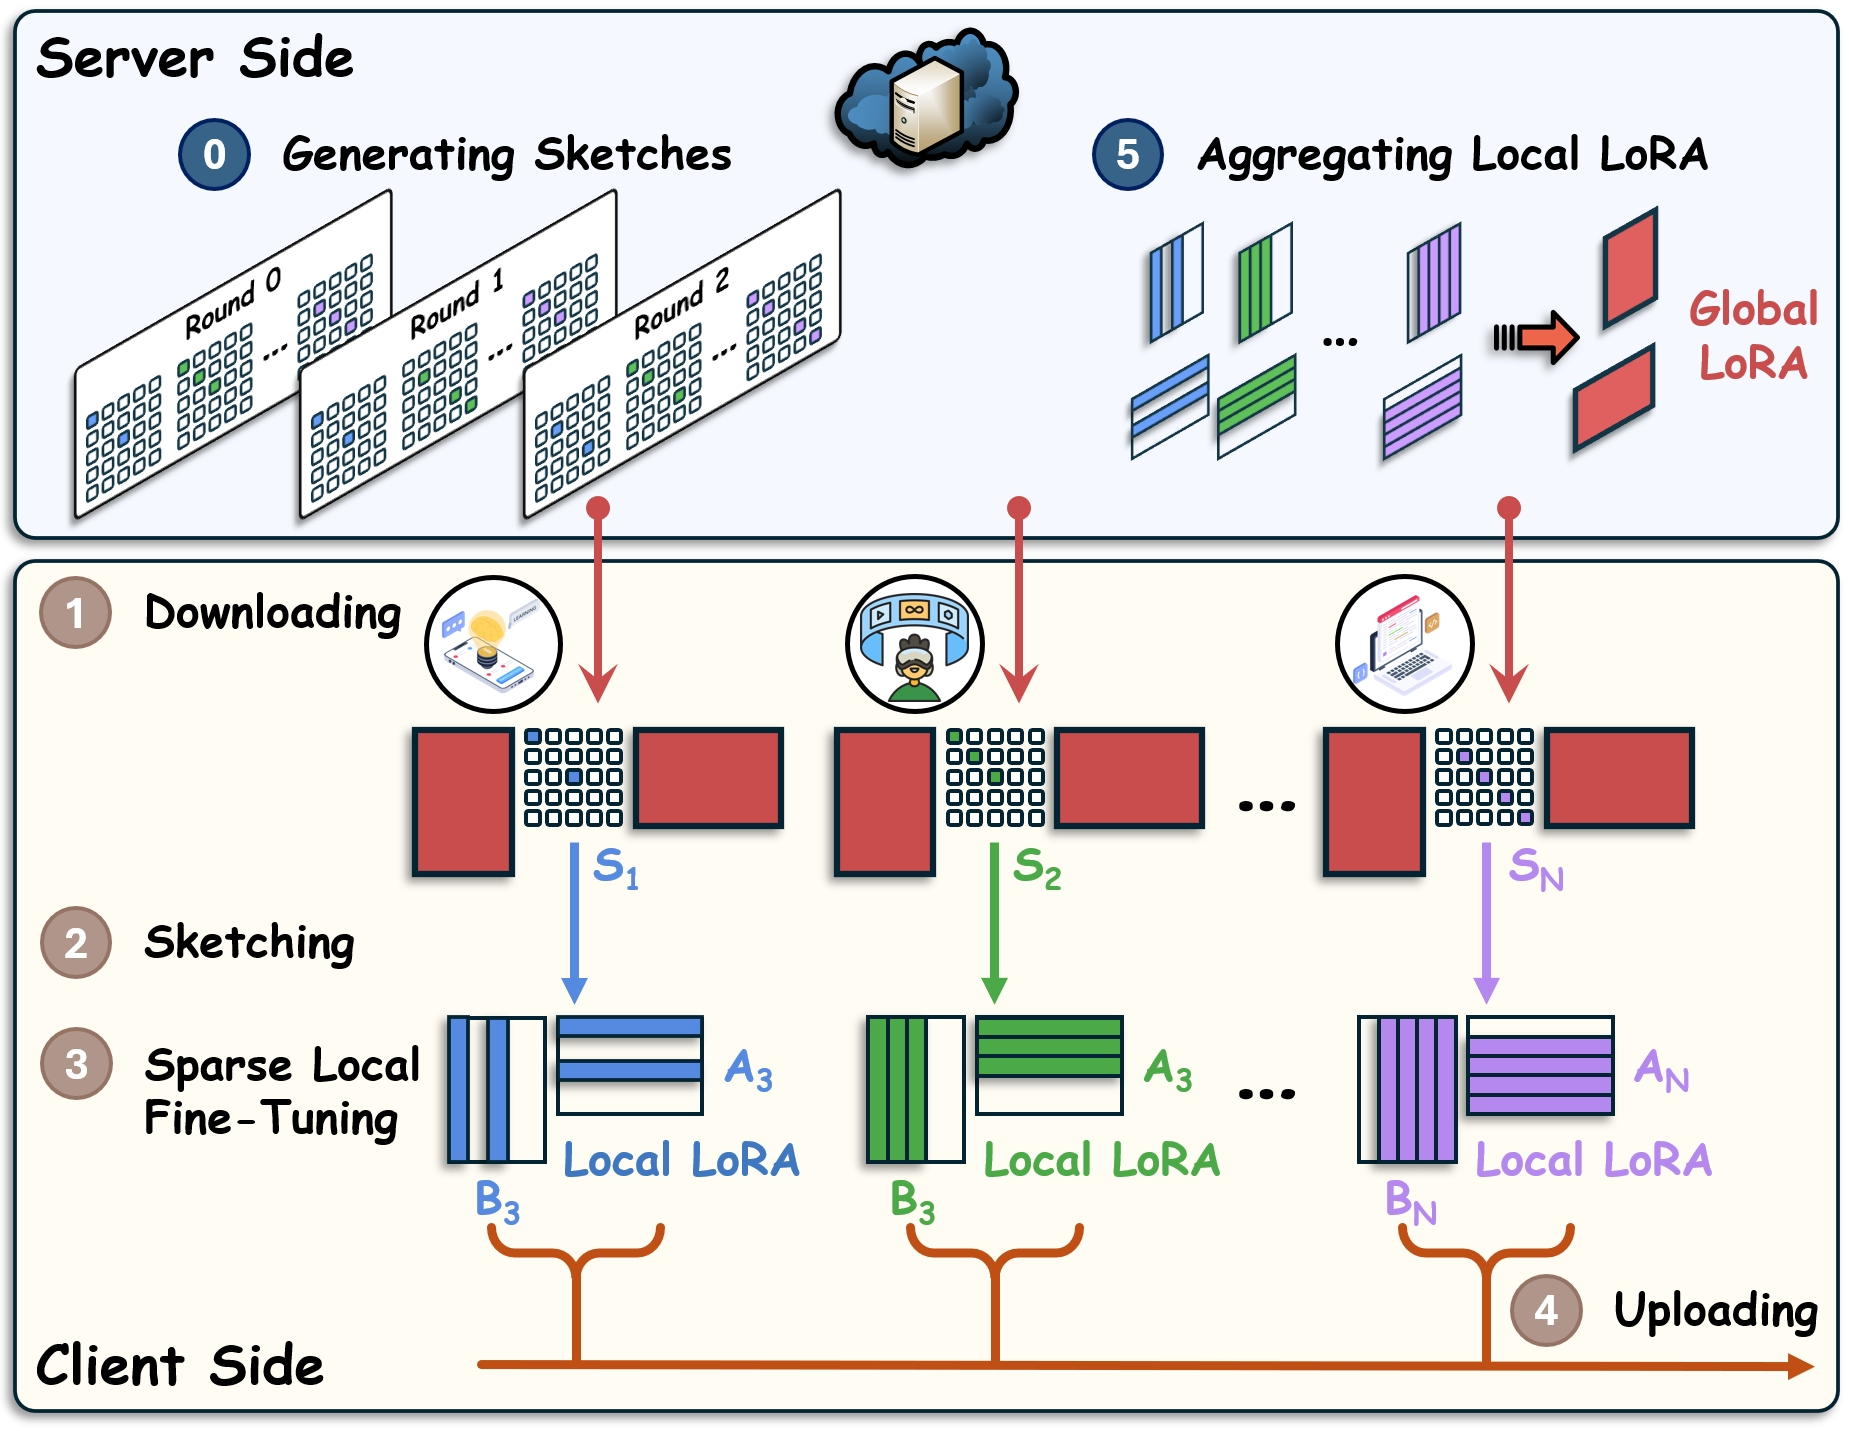
\includegraphics[width=.575\textwidth]{Figure/Overview.png}
    \end{center}
    \vspace{-3mm}
    \caption{\small An illustration of our proposed methodology where the server maintains a pair of global LoRA modules while the clients adaptively update submatrices of the global LoRA modules through sketching during each round.}
\label{fig:Motivation}
    \vspace{-2.6mm}
\end{wrapfigure}

Motivated by these limitations, this work develops a methodology for efficient federated LLM fine-tuning that (i) retains the flexibility of LoRA, (ii) provides theoretical convergence guarantees, and (iii) addresses the challenges posed by heterogeneous and constrained resources across distributed clients. As depicted in Figure \ref{fig:Motivation}, our key idea is to introduce a sketching-based LoRA update to the local fine-tuning, which allows clients to selectively update a subset of columns and rows of the LoRA modules during each round, reducing the computation and communication consumption. Additionally, our method customizes the fine-tuning process by adjusting the sparsity level of the sketching matrix, i.e., the size of the updated submatrices for each client in each iteration. As we will see, the impact of the introduced sketching mechanism on the overall optimization landscape requires careful modeling consideration, posing additional challenges for the theoretical analysis that we address in this work.

Overall, we make the following contributions:
\begin{itemize}[topsep=0pt,itemsep=4pt,parsep=0pt, partopsep=0pt, leftmargin=*]
    \item %We introduce FSLoRA, a resource-adaptive algorithm for collaborative on-device LLM fine-tuning. By leveraging configurable sketching matrices, FSLoRA provides flexible control over local computation and communication overhead, allowing distributed devices to optimize their update matrices based on resource constraints. 
    We propose federated sketching LoRA (FSLoRA), which leverages a sketching mechanism to enable clients to selectively update submatrices of global LoRA modules maintained by the server. By adjusting the sketching ratios, which determine the ranks of the submatrices on clients, FSLoRA effectively adapts to client-specific communication and computational constraints. 
    \item We present a rigorous convergence analysis of FSLoRA under non-uniform submatrix update scenarios (i.e., heterogeneous LoRA configurations) across clients, revealing how the sketching ratios affect the convergence rate via scaled smoothness constants. 
    %\textcolor{magenta}{I think we can provide some interesting or non-trivial insights in 1-2 sentences.} 
    Further, our results show that while increasing the sketching ratios improves convergence theoretically, it also raises communication and computation costs, suggesting a potential trade-off in selecting the sketching ratios.
    \item %We evaluate FSLoRA on a wide range of datasets and models with diverse parameter settings, consistently showing that FSLoRA outperforms existing solutions for collaborative on-device LLM fine-tuning in the federated system with heterogeneous resource distribution.
    We conduct extensive experiments across multiple datasets and LLM models with diverse parameter settings, demonstrating FSLoRA's superior performance compared to various baselines in accuracy, training time, and resource utilization. Our ablation studies further validate the effectiveness of the sketching mechanism and the ability of clients to exploit larger global ranks under FSLoRA.
\end{itemize}



%Concretely, to reduce communication and computation overhead, our approach involves updating only smaller subtensors of the LoRA modules during each iteration. By using a sketching matrix (see Figure \ref{fig:Motivation}), which acts as a filter, we decrease the volume of information transferred between edge devices and the server, making the implementation of distributed LLM systems across large amount of edge devices more practical. Additionally, recognizing the diverse computational capabilities across edge devices, we introduce a resource-adaptive strategy for fine-tuning. Instead of uniformly applying the same updates across all devices, our method customizes the fine-tuning process by adjusting the sparsity level of the sketching matrix, i.e., the size of the updated subtensor for each device in each iteration, as demonstrated in Figure \ref{fig:Motivation}. On the other hand, the use of non-uniform LoRA modules introduces extra challenge for the theoretical analysis. We thoroughly investigate this problem and make the following contributions:

% \begin{figure}[t]
%     \centering
%     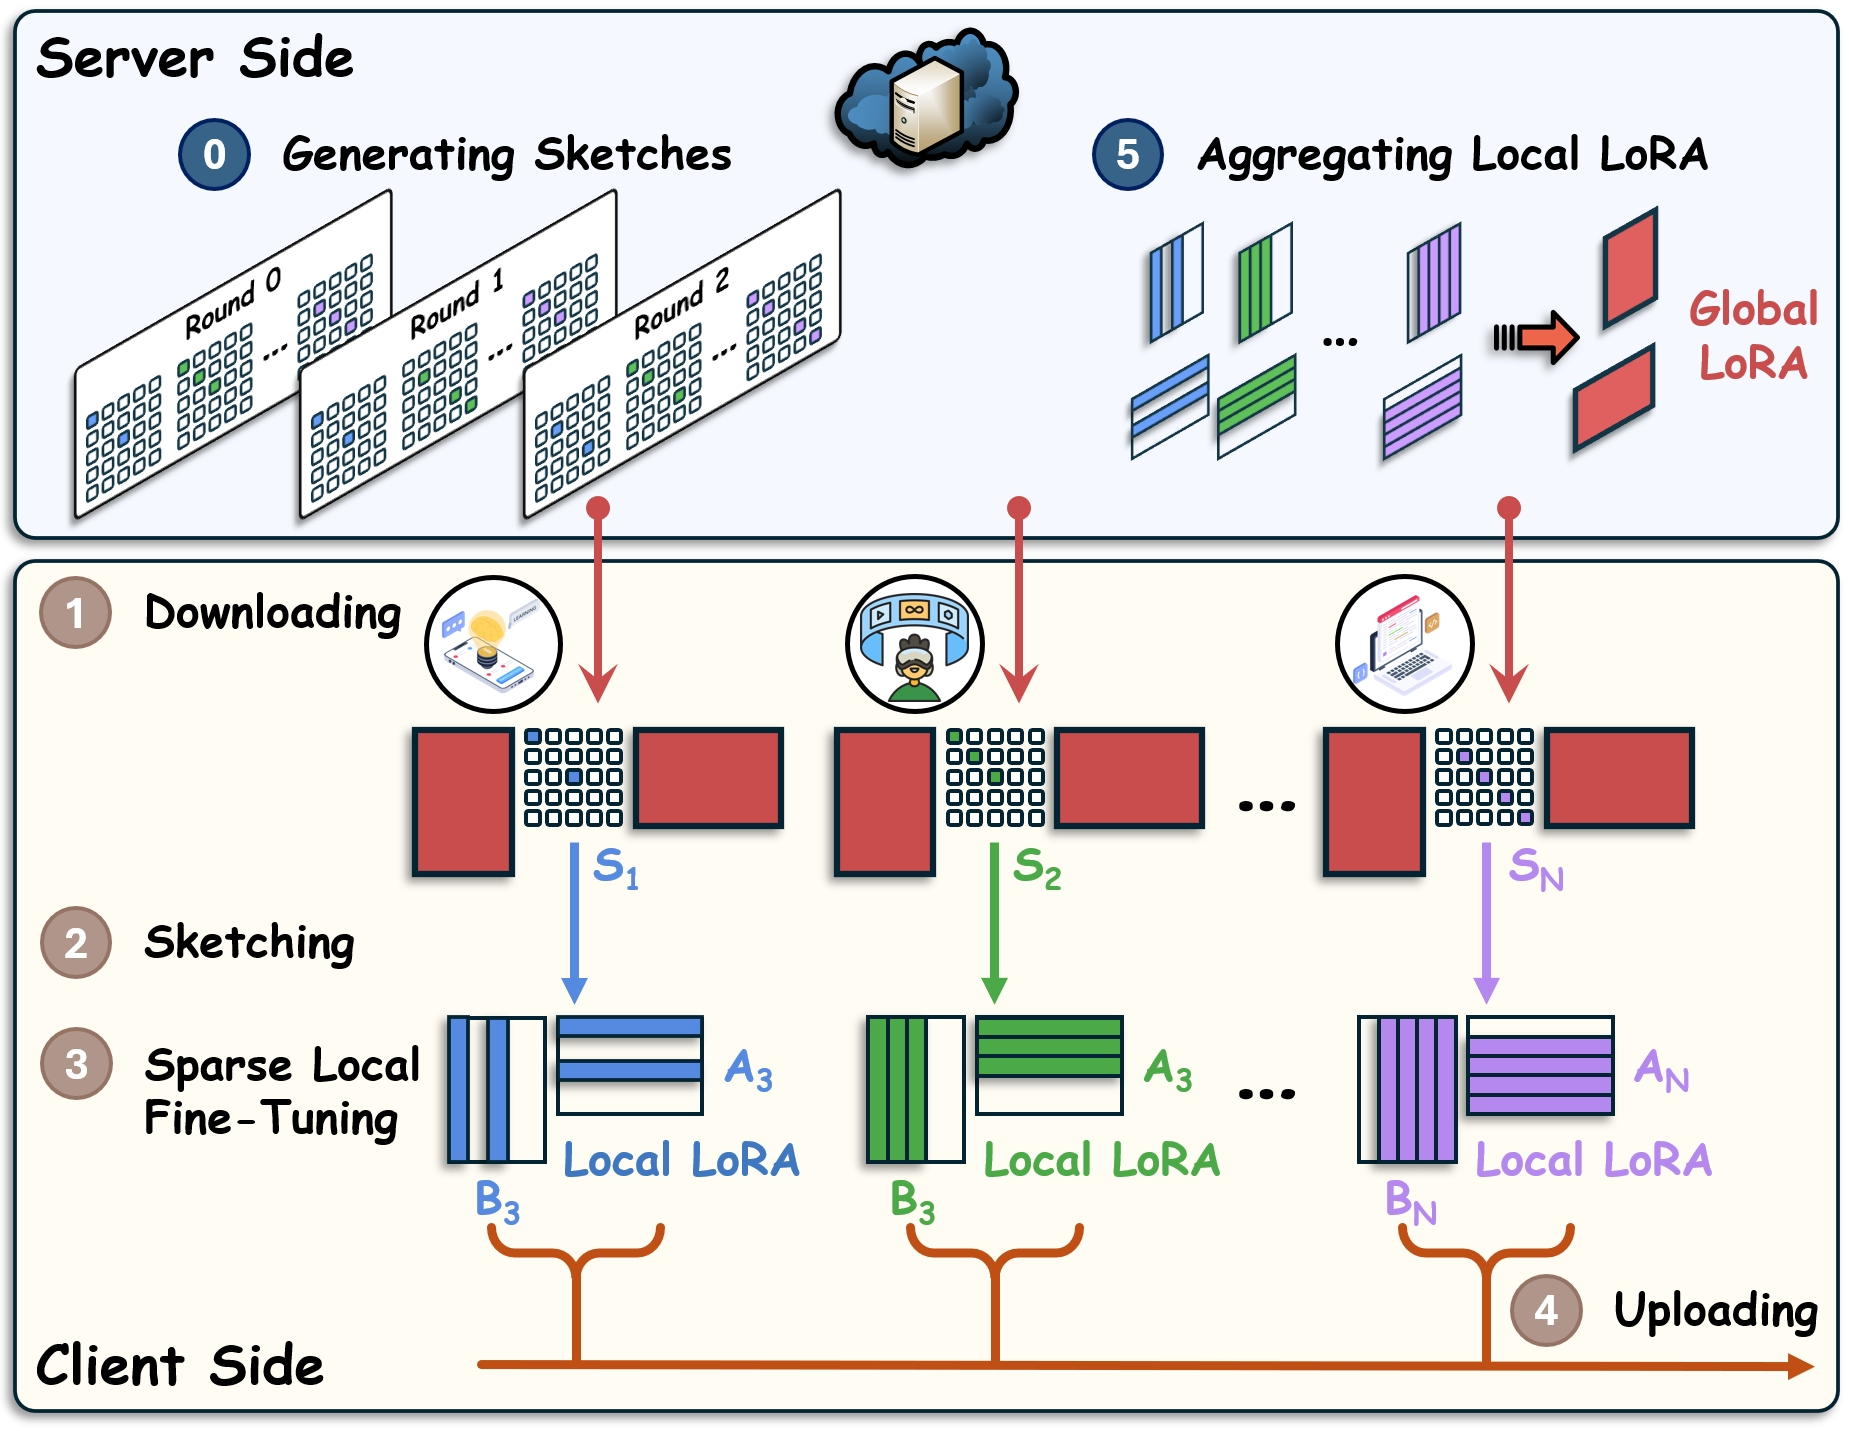
\includegraphics[width=\linewidth]{Figure/Overview}
%     \caption{An illustration of our proposed methodology where the server maintains a pair of global LoRA modules while the devices adaptively update submatrices of the global LoRA modules through sketching during each round.}
%     \label{fig:Motivation}
%     \vspace{-2mm}
% \end{figure}


\vspace{-1mm}

\subsection{Related Works}
\vspace{-1mm}

\begin{comment}
\textbf{LoRA-based parameter-efficient fine-tuning:}
%Building on the hypothesis that weight updates from the pre-trained model to specific tasks exhibit a low intrinsic rank, LoRA was proposed as a parameter-efficient approximation for full model fine-tuning \citep{hu2021lora}. Due to its superior performance, there has been a growing body of work focused on further improving LoRA.
LoRA was introduced in \citep{hu2021lora} as a parameter-efficient alternative to full model fine-tuning via low-rank matrix approximations.
Subsequently, \citet{kalajdzievski2023rankstabilizationscalingfactor} proposed rank-stabilized LoRA (rsLoRA), an approach that enhances LoRA's performance in high-rank scenarios by modifying the scaling factor applied to each low-rank product. \citet{shuttleworth2024lora} demonstrated that with this design, rsLoRA can approach the performance of full model fine-tuning as the rank of LoRA modules increases. 
\citet{han2024sltrain} introduced a sparse matrix in parallel with LoRA modules to improve the overall adaptation capability.
%\citet{lialin2023relora,xia2024chain} proposed ReLoRA and Chain of LoRA, respectively, allowing effective high-rank fine-tuning through successive low-rank updates. Extending this line of work, \citet{malinovsky2024randomized} introduced a modified sequential LoRA adaptation framework and established its convergence guarantees.
In \citep{lialin2023relora,malinovsky2024randomized,xia2024chain}, the authors proposed sequential low-rank adaptation schemes, including ReLoRA and CoLA, to enable high-rank fine-tuning through iterative low-rank updates.
However, the works mentioned above focus on centralized scenarios, assuming that the data required for fine-tuning is available at the server.
\end{comment}


\textbf{Collaborative fine-tuning via federated LoRA:} Federated LoRA is an efficient approach for collaborative LLM fine-tuning among distributed clients \citep{chen2023federated,sun2024improving,guo2025selectiveaggregationlowrankadaptation}. Building on this foundation, \citet{kuo2024federatedlorasparsecommunication} proposed integrating communication compression with federated LoRA to further reduce communication overhead. Meanwhile, \citet{bai2024federatedfinetuninglargelanguage,cho2024heterogeneouslorafederatedfinetuning,byun2024towards,wang2024flora,koo2024robustefficientfederatedlowrank} explored the challenges of resource heterogeneity across distributed clients and introduced heterogeneous LoRA as a solution.
However, the approaches proposed in \citep{cho2024heterogeneouslorafederatedfinetuning,koo2024robustefficientfederatedlowrank,byun2024towards,bai2024federatedfinetuninglargelanguage} lack a theoretical foundation. Moreover, the FlexLoRA method introduced in \citep{bai2024federatedfinetuninglargelanguage} incurs additional computational overhead due to its reliance on singular value decomposition (SVD). Furthermore, the FLoRA algorithm proposed in \citep{wang2024flora} requires the clients to merge the LoRA modules into the base model, thereby compromising the inherent flexibility of LoRA. Overall, there is still a lack of a systematic and theoretically grounded solution that can effectively tackle heterogeneous collaborative LLM fine-tuning.

%\textbf{Effectiveness of Higher-Rank LoRA Modules.}
\textbf{Enhancing adaptability via higher-rank LoRA modules:}
The foundational study by \citet{hu2021lora} demonstrated that small ranks can be sufficient for certain tasks; however, they also acknowledge that small rank LoRA modules may not work universally, especially when the downstream task differs significantly from pretraining. Following this, several works explored the effect of increasing the rank in LoRA modules. In a centralized setup, \citet{kalajdzievski2023rankstabilizationscalingfactor} and  \citet{shuttleworth2024lora} showed that higher-rank LoRA models can closely approximate full fine-tuning under rsLoRA. In a federated LLM fine-tuning regime, \citet{bai2024federatedfinetuninglargelanguage} demonstrated improved performance with larger ranks under FlexLoRA. 
%Similarly, \citet{cho2024heterogeneouslorafederatedfinetuning} reported that increasing LoRA rank can lead to better performance initially, but eventually will overfit. They also showed that by applying some tricks, e.g., rank-pruning, overfitting can be mitigated and HeteroLoRA can enjoy the benefit of larger ranks. 
Similarly, \citet{cho2024heterogeneouslorafederatedfinetuning} reported that, with proper overfitting control, HeteroLoRA can also benefit from larger ranks.
Overall, while small ranks may suffice for simpler tasks or strong base models, higher-rank modules are necessary to compensate for limited backbone capability, such as in lightweight LLMs, and to enable effective adaptation to more complex downstream tasks.


\textbf{Sketching-based optimization:} Sketching is an efficient technique for mitigating the complexity of high-dimensional optimization, with its earliest applications in least-squares regression \citep{sarlos2006improved,wang2022iterative}. Beyond this, gradient sketching has been employed to construct preconditioners for gradient descent methods \citep{gower2015randomized}. Building on these foundations, recent work has applied sketching to distributed optimization. In particular, \citet{charalambides2024distributed} proposed hybrid local-global sketching for distributed least-squares, while \citet{demidovich2023mast} developed a distributed sparsified training framework based on sketching. \citet{shrivastava2024sketching} demonstrated that sketching substantially reduces communication in distributed training of overparameterized deep models without sacrificing accuracy.
%\citet{nicolas2025communication} introduced correlation-aware sketches that simultaneously reduce communication and differentially private noise. 
More recently, \citet{nicolas2025communication} investigated sketching-based differential privacy and demonstrated its compatibility with secure aggregation.
Despite these advances, sketching strategies tailored to structured low-rank adaptation modules such as LoRA remain largely unexplored.

%\textcolor{red}{Try to get Sec. 2 to start close to top of page 2. Can reduce abstract size, and intro before Challenges.}



\begin{comment}
Large language models (LLMs) have recently achieved remarkable success across a wide range of fields, including machine translation, generative AI, and natural language understanding. This success is driven by the substantial increase in both model parameters and training dataset volume. With vast datasets, LLMs can learn broad linguistic patterns, semantics, and even contextual nuances, enabling them to perform effectively across diverse tasks. While LLMs show impressive zero-shot performance across many tasks, fine-tuning remains essential for certain applications, particularly for specialized or domain-specific tasks. 
Although fine-tuning requires much fewer computational resources compared to pre-training, the memory cost would be still a hard barrier for full model fine-tuning. For instance, fine-tuning a full LLaMA 7B model with a single batch size requires at least $58$ GB memory ($14$ GB for
trainable parameters, $42$ GB for Adam optimizer states and
weight gradients, and $2$ GB for activations. 
To tackle this, many parameter-efficient fine-tuning methods have been proposed, such as prompt tuning, inserting adapters sequentially, and adding trainable Low-Rank Adaptation (LoRA) modules, etc. This work will focus on LoRA due to its implementation efficiency and promising performance. 

The key motivation behind LoRA is the hypothesis that the updates to the weights from the pre-trained model to specific tasks have a low intrinsic rank during adaptation. Out of its superior performance, LoRA has attracted much attention recently. Inspired by the success of LoRA, tremendous efforts have been devoted to further improving fine-tuning, even the pre-training, performance from a low-rank update perspective, evidenced by algorithms like rsLoRA, ReLoRA, Chain of LoRA, sparse plus LoRA, and etc.
For instance, \citep{kalajdzievski2023rankstabilizationscalingfactor} proposed a scaling factor which makes LoRA enjoy a better performance as the ranks of LoRA modules increase. ReLoRA and Chain of LoRA impart the idea of residual learning into LoRA, which periodically merges the learned LoRA modules into the full model and re-initializes the LoRA modules for a new round of tuning. 
However, the works mentioned above mainly consider centralized scenarios and assume the data required for fine-tuning is available at the central server. Nevertheless, in some scenarios, the data are distributed across edge devices and not available to the central server due to privacy concerns. To bridge this gap, federated LoRA was proposed, which aims to allow multiple edge devices to collaboratively fine-tune an LLM without compromising data privacy while still enjoying the benefit of efficiency brought by LoRA. 

The incorporation of LoRA into federated learning effectively reduces the number of parameters that need to be tuned among distributed edge devices. However, the communication load over networks during model aggregation could still bottleneck the fine-tuning efficiency for the system with communication resource-constrained mobile devices, especially when the rank of LoRA modules is set to be a large number. In addition, system heterogeneity among clients raises extra problems for the implementation of federated LoRA. Concretely, the computation and communication resources vary among edge devices, which makes setting uniformly ranked LoRA modules across edge devices impractical. Motivated by this observation, \citep{} developed heterogeneous LoRA which lets edge devices update non-uniformly ranked LoRA modules. Concretely, clients with lower-rank models have their models padded to match the higher ranks before aggregation. During the model dissemination stage, clients with lower resources receive a truncated global model. However, this heuristic padding and truncation make the convergence of heterogeneous federated LoRA hard to be guaranteed. More recently, a variant of LoRA called federated stack LoRA was proposed to fix this convergence issue. However, it requires the clients to periodically update the original full model, which may violate the memory constraint of edge devices. Moreover, one of LoRA's key advantages is the ability to switch between different LoRA modules for multiple downstream tasks without altering the base model. Merging the modules into the original weights makes the model specialized for a single task, sacrificing this flexibility.

Despite many efforts that have been made by existing literature, there remains a lack of a systematic and theoretically grounded solution that preserves the advantages of LoRA while effectively addressing the challenges posed by heterogeneous federated learning environments with resource-constrained clients.
\end{comment}

\vspace{-1.5mm}
\section{Problem Background}\label{sec:background}
\vspace{-1.5mm}

%\subsection{Preliminaries}
\subsection{LoRA-based Federated LLM Fine-tuning}\label{sec:background:fedlora}
\vspace{-1mm}
%\textbf{LLM Fine-tuning with LoRA:} LLM fine-tuning adapts a pre-trained model to specific tasks, improving performance without full retraining. Let \( {\bf W}_0 \in \mathbb{R}^{m \times n} \) represent the parameter of the pre-trained model.  Conventional full model fine-tuning learns a dense update matrix \( \Delta {\bf W} \in \mathbb{R}^{m \times n} \), updating the model as \( {\bf W} = {\bf W}_0 + \Delta {\bf W} \). Though effective, it is computationally intensive due to the need to update all parameters. LoRA \citep{hu2021lora} addresses this challenge by approximating the weight update matrix \(\Delta {\bf W}\) with a low-rank decomposition. Instead of updating \(\Delta {\bf W}\) directly, it is represented as: \( \Delta {\bf W} =  {\bf B} {\bf A} \) where \( {\bf B} \in \mathbb{R}^{m \times r} \) and \( {\bf A} \in \mathbb{R}^{r \times n} \), with rank \( r \ll m, n \). The complete weight update in LoRA can be expressed as \({\bf W} = {\bf W}_0 +  \bf{BA}\). 


%Let the original model weights be denoted by \( {\bf W}_0 \in \mathbb{R}^{m \times n} \). The conventional full model fine-tuning involves learning a full-size update \( \Delta {\bf W} \in \mathbb{R}^{m \times n} \), so that the updated model \( {\bf W} = {\bf W}_0 + \Delta {\bf W} \) work well on some downstream task. Typically, \( \Delta {\bf W} \) is dense and requires updating all parameters, which can be computationally expensive for large models. LoRA builds on the assumption that \( \Delta {\bf W} \) has a low-rank structure, meaning that it can be approximated by two smaller low-rank matrices. Specifically, instead of directly learning \( \Delta {\bf W} \), LoRA decomposes it as: \(\Delta {\bf W} = \bf{BA}\), where \( \bf{B} \in \mathbb{R}^{m \times r} \) and \( \bf{A} \in \mathbb{R}^{r \times n} \), and \( r \ll m, n \). This low-rank decomposition efficiently reduces the number of trainable parameters, making fine-tuning more efficient while still capturing the necessary changes to the model. The full weight update in LoRA is thus: \({\bf W} = {\bf W}_0 +  \bf{BA}\). The reparameterized optimization problem within LoRA fine-tuning can be expressed \begin{equation}\label{lora_formulation}\min_{{\bf{B}} , {\bf{A}}} f({\bf{B}}, {\bf{A}}) \eqdef \mathbb{E}_{\xi \sim \mathcal{D}} \left[ \ell ({{\bf W}}_0 + {\bf{B}} {\bf{A}}, \xi)\right],\end{equation} where $f$ denotes the empirical loss, \({\bf W}_{0}\) denotes the pretrained model, ${\bf B} \in \mathbb{R}^{m\times r},  {\bf A}\in \mathbb{R}^{r\times n}$ are LoRA modules, \(\ell\) is the sample-wise loss function, and \(\mathcal{D}\) is the dataset used for fine-tuning.

%\textbf{Federated LoRA for Collaborative Fine-tuning:} 
%\textbf{LoRA-based Federated LLM Fine-tuning:} 
The federated LoRA fine-tuning problem can be formulated as 
\vspace{-0.05in}
\begin{equation}\label{fed_lora_formulation}
\begin{aligned}
    \min_{\bf{B}, \bf{A}} f({\bf B},{\bf A}) \eqdef \frac{1}{N} \sum_{i=1}^{N} f_i({\bf B},{\bf A}), ~\text{where}~
    f_i({\bf B},{\bf A}) \eqdef  \mathbb{E}_{\xi \sim \mathcal{D}_i} \left[ \ell ({\bf W}_{0} + {\bf B} {\bf A}, \xi)\right],
\end{aligned}
\end{equation}
where \({\bf W}_{0}\) denotes the frozen base model, ${\bf B} \in \mathbb{R}^{m\times r},  {\bf A}\in \mathbb{R}^{r\times n}$ are LoRA modules, \(N\) denotes the number of clients, \(\xi\) denotes a data sample, and \(\mathcal{D}_i\) is the local dataset on client \(i\). 
\(\ell\), \(f_i\), and \(f\) are the sample loss function, the local loss for client \(i\), and the global loss, respectively. 

Problem \eqref{fed_lora_formulation} aligns with the conventional federated optimization formulation, which thus can be solved using the FedAvg algorithm. 
Based on the FedAvg framework, \citet{zhang2024towards} developed federated LoRA, which applies a uniform rank \(r\) across all clients, overlooking resource heterogeneity. 
This one-size-fits-all approach leads to resource mismatches, where computationally constrained clients may struggle, while more powerful clients remain underutilized with a fixed rank.

\begin{comment}
Based on the FedAvg framework, \citet{zhang2024towards} developed a FedLoRA algorithm, which comprises of the following procedures:
\begin{itemize}[topsep=0pt,itemsep=4pt,parsep=0pt, partopsep=0pt, leftmargin=*]
    \item  Local Update: Each client independently fine-tunes their respective LoRA modules \({\bf B}_i\) and \({\bf A}_i\) through stochastic gradient descent based on local datasets. 
    \item Global Aggregation: The server aggregates local updates by averaging these updated low-rank modules \(\frac{1}{N} \sum_{i=1}^{N} {\bf{B}}_i\) and \(\frac{1}{N} \sum_{i=1}^{N} {\bf{A}}_i\), separately.
    \item LoRA Modules Dissemination: The central server disseminates the averaged LoRA modules to clients, which will then be used to initialize local LoRA modules at each client \( {\bf{B}}_i \leftarrow \frac{1}{N} \sum_{i=1}^{N} {\bf{B}}_i\) and \( {\bf{A}}_i \leftarrow \frac{1}{N} \sum_{i=1}^{N} {\bf{A}}_i\) for the next round of fine-tuning. 
\end{itemize}
\end{comment}
%\begin{remark}[NAME]Beyond what we discussed above, there is another variant of federated LoRA proposed by \citep{sun2024improving}, where the authors claimed that the server is interested in \(\sum_{i} {\bf{B}}_i {\bf{A}}_i\). Due to \( \frac{1}{N} \sum_{i} {\bf{B}}_i {\bf{A}}_i \neq (\frac{1}{N} \sum_{i=1}^{N} {\bf{B}}_i) (\frac{1}{N} \sum_{i=1}^{N} {\bf{A}}_i) \), separately aggregating \({\bf{B}}_i\) and \({\bf{A}}_i\) and then broadcasting them back to clients to initialize the next round of fine-tuning could potentially introduce convergence issues and proposed to fix \({\bf{A}}_i\) for all the clients and only update \({\bf{B}}_i\). However, it is worth noting that the original federated LoRA can converge to the same quality solution as LoRA in the centralized setup based on some common assumptions such as bounded gradient similarity and smoothness. Specifically, for a general non-convex smooth function \(f(\bf B,{\bf A})\), under the LoRA formulation \eqref{lora_formulation}, it is well known that the gradient descent algorithm will converge a stationary point of \(f(\bf B,{\bf A})\). On the other hand, under the federated LoRA formulation \eqref{fed_lora_formulation}, we can anticipate that the FedAvg algorithm, i.e., FedLoRA, achieves the stationary point of $f(\bf B,{\bf A})$ \citep{karimireddy2020scaffold}. \end{remark}


\begin{comment}
In this paper, we want to argue for the original federated LoRA. We show in Proposition ??? that the original federated LoRA can converge to the same quality solution as that of LoRA in the centralized setup. 
\begin{proposition}
    Seperately aggregation can achieve the same quality solution as Federated LoRA. 
\end{proposition}
\end{comment}

\begin{comment}
\subsection{Challenge of FedLoRA}
While \textcolor{blue}{FedLoRA} reduces communication costs by only transmitting low-rank parameter updates, several fundamental challenges emerge in practical deployments:

\textbf{Device Heterogeneity and Fixed Rank Selection:} FedLoRA applies a uniform rank \(r\) across all edge devices which thus fails to address the inherent heterogeneity in federated learning environments. This one-size-fits-all approach creates the issue of resource mismatch where computationally constrained devices may struggle with higher ranks, while powerful devices remain underutilized with lower ranks. 

\textbf{Communication Bottlenecks:} Despite the parameter reduction achieved through low-rank decomposition, FedLoRA still faces significant communication challenges:
1) The communication cost scales linearly with rank $r$, becoming substantial when higher ranks are necessary for complex tasks.
2) Collaborative on-device LLM fine-tuning necessitates frequent parameter communication since mobile devices have limited memory that constrains batch sizes, while fine-tuning datasets are often quite large, requiring more training iterations to go through the whole dataset. This combination means each device can only process a small number of samples before needing to synchronize parameters, leading to frequent communication rounds to maintain training stability.
\end{comment}

 \vspace{-1mm}

\subsection{Aren't the Existing Solutions Good Enough?}\label{sec:limitations_of_existing}
%\subsection{Limitations of Other Federated LoRA Approaches}
\vspace{-1mm}

To address this issue, researchers have proposed heterogeneous federated LoRA approaches, where clients maintain non-uniform LoRA modules with varying ranks. They also introduce mechanisms to overcome the challenges of directly aggregating matrices with different dimensions.   
However, these methods often lack theoretical foundation or incur additional computational and memory overhead.
%However, these methods either lack theoretical justification or introduce additional computational and memory overhead, as outlined below.

%\textbf{HeteroLoRA \citep{cho2024heterogeneouslorafederatedfinetuning}} tries to addresses the aforementioned challenges by allowing \textcolor{blue}{edge devices} to update non-uniform LoRA modules. \textcolor{blue}{Devices} with smaller rank modules pad their updates to match the size of the largest modules before aggregation. During global model dissemination, resource-constrained devices receive a truncated version of the global model. HeteroLoRA, while easy to implement, is largely heuristic and lacks a rigorous theoretical foundation. Additionally, its dependence on zero-padding diminishes optimization efficiency, potentially limiting overall performance.
\textbf{HeteroLoRA \citep{cho2024heterogeneouslorafederatedfinetuning}} lets the server pad the updates from the clients with smaller ranks to match the size of the largest rank during aggregation. During model dissemination, clients receive a truncated version of the global LoRA modules from the server. Although easy to implement, HeteroLoRA is primarily heuristic in nature and lacks a rigorous theoretical foundation, potentially limiting its performance, as we will see in Section \ref{sec:experiment}.
%HeteroLoRA, while easy to implement, lacks a solid theoretical foundation. Additionally, its dependence on zero-padding diminishes optimization efficiency, potentially limiting overall performance.

%\textbf{FlexLoRA \citep{bai2024federatedfinetuninglargelanguage}} introduces an alternative approach where the server first collects the individual LoRA matrices $\mathbf{B}_i $ and $ \mathbf{A}_i$ from edge devices and then computes the product $\mathbf{B}_i \mathbf{A}_i$ for each device and averages these products. To enable non-uniform initialization of LoRA modules, the server applies truncated singular value decomposition (SVD) to the averaged product $\frac{1}{N} \sum_{i=1}^N \mathbf{B}_i \mathbf{A}_i$. Although FlexLoRA supports heterogeneous LoRA updates, the use of truncated SVD introduces significant computational and memory overhead on the server. Additionally, the approximation errors resulting from the truncated SVD could undermine its effectiveness in certain scenarios.

\textbf{FlexLoRA \citep{bai2024federatedfinetuninglargelanguage}} requires the server to collect the individual LoRA matrices $\mathbf{B}_i $ and $ \mathbf{A}_i$ from the clients and then computes their product $\mathbf{B}_i \mathbf{A}_i$. To support the initialization of non-uniform LoRA modules, the server applies truncated SVD to the averaged product $\frac{1}{N} \sum_{i=1}^N \mathbf{B}_i \mathbf{A}_i$. However, this approach introduces extra computational and memory overhead on the server due to truncated SVD, and the associated error can limit the performance as demonstrated in Section \ref{sec:experiment}.
   
%\textbf{FLoRA \citep{wang2024flora}} employs a stacking mechanism where the server concatenates the LoRA modules from distributed devices \(\mathbf{B}_1, \ldots, \mathbf{B}_N\) along the second dimension and \(\mathbf{A}_1, \ldots, \mathbf{A}_N\) along the first dimension. The concatenated matrices are then disseminated to the devices, where each device computes their product and merges it into the base model. Following that, the devices randomly initialize new LoRA modules for the next round of local fine-tuning. However, the communication complexity of FedStack grows linearly with the number of the devices due to the need to transmit these concatenated matrices.  Additionally, the devices are required to compute the product of the concatenated matrices and merge them into the base model, leading to increased computation and memory demands. This approach also compromises the inherent flexibility of LoRA, which allows a base model to accommodate multiple LoRA adapters tailored to different tasks.

\textbf{FLoRA \citep{wang2024flora}} introduces a stacking mechanism where the server concatenates LoRA modules from the clients. The concatenated matrices are then sent back to the clients, which compute their product and merge it into the base model before initializing new LoRA modules for the next fine-tuning round. However, this approach increases communication complexity linearly with the number of clients, imposes higher computation and memory demands on the clients, and compromises LoRA's flexibility to support multiple adapters for different tasks.

More detailed comparisons on computation, memory, and communication are presented in Appendix \ref{appen:com_memo_comparison}.
In summary, a theoretically-grounded solution that preserves LoRA's benefits while effectively addressing resource heterogeneity across distributed clients remains lacking. 
\vspace{-1.5mm}


\section{Federated Sketching LoRA} 
\vspace{-0.5mm}

Motivated by the limitations of existing methods, we propose a new federated LoRA reformulation. Building on this foundation, we develop FSLoRA, a heterogeneous LoRA algorithm that preserves LoRA's flexibility while accommodating client resource heterogeneity.


%Motivated by the limitations of existing methods, we proposed a resource-adaptive algorithm, FSLoRA, which allows each device to update submatrices of the full modules \( \mathbf{B} \) and \( \mathbf{A} \) at each round. The introduced sketching mechanism enables the adaptive selection of submatrix sizes for the devices based on their resource constraints.

%The introduced sketching mechanism enables the adaptive selection of submatrix sizes for edge devices based on their resource constraints, which will be detailed in Section \ref{sec:heterogeneous}. The overview of FSLoRA is shown in Figure \ref{fig:Motivation} and Algorithm \ref{alo_flora}. 

\subsection{Our Formulation}

We propose a sketching-based LoRA formulation for collaborative LLM fine-tuning as follows: 
\vspace{-0.05in}
\begin{equation}\label{lora_formulation_ours}
\begin{aligned}
\min_{{\bf B},{\bf A}} f^{\mathcal{S}}({\bf B},{\bf A}) \eqdef  \frac{1}{N} \sum_{i=1}^N f_i^{\mathcal{S}} ({\bf B},{\bf A}) ~\text{where}~
f_i^{\mathcal{S}}({\bf B},{\bf A}) \eqdef  \mathbb{E}_{ {\bf S} \sim \mathcal{S}_i; \xi \sim \mathcal{D}_i} \left[ \ell ({\bf W}_{0} + {\bf B}\bf S{\bf A}, \xi)\right],
\end{aligned}
\end{equation}
where ${\bf B} \in \mathbb{R}^{m\times r},  {\bf A}\in \mathbb{R}^{r\times n}$ are LoRA modules, $f_i^{\mathcal{S}}$ is the local loss function at client $i$ with sketching, and \({\bf S}\) denotes a sketching matrix randomly sampled from the diagonal matrix set \(\mathcal{S}_i = \mathcal{S}(r, k_i)\). The set \(\mathcal{S}(r, k_i)\) comprises diagonal matrices of size \(r \times r\) with exactly \(k_i\) non-zero entries. 
%where ${\bf W}_{0}$ denotes the pre-trained model, ${\bf B} \in \mathbb{R}^{m\times r},  {\bf A}\in \mathbb{R}^{r\times n}$ are LoRA modules, \(\ell\) is the sample-wise loss function, \(\mathcal{D}_i\) is the local dataset of device \(i\), and \(\mathcal{S}_i\) represents the sketching matrix set for device $i$. 
The formal definition of \(\mathcal{S}(r, k)\) is provided below:
\begin{definition}[Random-$k$ sketching]\label{skeching_def}
A random-$k$ diagonal matrix set is defined as:  
\[
\mathcal{S}(r, k) \!=\! \Bigg \{ \! \mathbf{S} \!\mid \! \mathbf{S} \!=\! \frac{r}{k} \! \sum_{j \in \mathcal{I}} \! \mathbf{e}_j \mathbf{e}_j^\top, \, \mathcal{I} \subseteq \{1, \ldots, r\}, \, |\mathcal{I}| \!=\! k \Bigg \},
\]  
where \(\mathbf{e}_1, \dots, \mathbf{e}_r \in \mathbb{R}^r\) are standard unit basis vectors and index set \(\mathcal{I}\) is a random subset of \([r] \eqdef \{1,2,\ldots, r\} \) sampled uniformly from all subsets of \([r]\) with cardinality \(k\).
\end{definition}

With \(\mathbf{S}\) being a matrix sampled from \(\mathcal{S}_i\), we have $
   \mathbf{BSA} = \frac{r}{k_i} \sum_{j \in \mathcal{I}_i} \mathbf{B} \mathbf{e}_j \mathbf{e}_j^\top \mathbf{A},
   $
where \(\mathcal{I}_i\) corresponds to the index set of non-zero diagonal entries of \(\mathbf{S}\). \(\mathbf{B} \mathbf{e}_j\) extracts the \( j \)-th column of \(\mathbf{B}\) while \(\mathbf{e}_j^\top \mathbf{A}\) extracts the \( j \)-th row of \(\mathbf{A}\). In other words, only \(k_i\) columns and rows in the LoRA modules \(\bf B\) and \(\bf A\) are activated by the sketching matrix in the loss \(\ell ({\bf W}_{0} + {\bf B}\bf S{\bf A}, \xi)\) at client \(i\).  On the other hand, the sketching matrix \(\bf S\) satisfies \(\mathbb{E}_{\mathbf{S} \sim \mathcal{S}_i}[\mathbf{S}] = \mathbf{I}_r\) where $\mathbf{I}_r$ is a $r$-dimensional identity matrix. Based upon this property, ${\bf W}_0 + {\bf B} {\bf S} {\bf A}$ can be treated as an unbiased estimate of ${\bf W}_0 + \bf B{\bf A}$. 
%The proposed formulation (i.e., \eqref{lora_formulation_ours}) serves as an approximation of the original federated LoRA formulation (i.e., \eqref{fed_lora_formulation}). 
%
%The idea behind sketching shares some similarities with LoRA Dropout \citep{lin2024loradropoutsparsityregularizer}. LoRA Dropout randomly drops some columns and rows of the LoRA modules to achieve sparsity regularization, effectively mitigating overfitting. Our goal is to leverage the sketching matrix to strike a balance between the large rank of global LoRA modules and the limitations of resource-constrained devices. Specifically, when \({\bf S}\) is a random diagonal sketching matrix, the local gradients with respect to the LoRA modules computed on the devices exhibit structured sparsity. This structured sparsity effectively reduces both the computational and communication overhead on the devices, as elaborated in the following subsection. 
%

\textbf{Intuition:} A larger rank allows LoRA modules to be more expressive, leading to better performance \citep{bai2024federatedfinetuninglargelanguage,kalajdzievski2023rankstabilizationscalingfactor,shuttleworth2024lora}. However, resource-constrained clients cannot afford the computational or communication demands of large-rank modules. Our formulation \eqref{lora_formulation_ours} leverages the sketching matrix to balance the expressiveness of high-rank LoRA modules with the resource constraints of different clients. With the sketching mechanism introduced, the local gradients with respect to the LoRA modules on the clients will exhibit structured sparsity. By adjusting the sketching ratio \(k_i/r\), we can tailor the sparsity of the gradient to match the capabilities of each client, ensuring affordable training while maintaining performance across heterogeneous systems, as elaborated in the following subsection. Overall, compared to \eqref{fed_lora_formulation}, our formulation offers a more flexible framework, tailored to address the diverse capabilities of heterogeneous clients.
%Overall, compared to \eqref{fed_lora_formulation}, our formulation offers a more flexible framework for resource-heterogeneous system.

%\textcolor{magenta}{Write a sentence something like: Compared to the original FL formulation in \eqref{fed_lora_formulation}, our new objective .....(provide some insights on the advantage? or say the it's detailed in the following subsection?) }

\subsection{Sparsity in the Gradients}
In this subsection, we analyze the gradient structure of LoRA modules and highlight the gradients' sparsity properties under a given sketching matrix. 
%under our reformulation
To begin, we present the gradient expressions for the LoRA modules \(\bf B\) and \(\bf A\) in the following lemma. The proof is provided in Appendix \ref{proof_compute_grad}.
\begin{lemma}[Gradient Formulation]\label{compute_grad}
For a given sketching matrix \(\bf S\), the gradients of  \( \ell(\bf W_0 + {\bf B}\bf S{\bf A}, \xi)\) with respect to ${\bf B}$ and ${\bf A}$ take the following form
%\tilde{\ell}(\bf B,{\bf A}, \xi) \eqdef
\begin{equation}\label{gradient_matrix}
\begin{aligned}
    {\nabla}_{\bf B} \ell({\bf W}_0 + {\bf B} {\bf S} {\bf A}, \xi) &= \nabla \ell({\bf W}_0 + {\bf B} {\bf S} {\bf A}, \xi)  {\bf A}^{\top} {\bf S}^{\top} \\
    {\nabla}_{\bf A} \ell({\bf W}_0 + {\bf B} {\bf S} {\bf A}, \xi) &= {\bf S}^{\top} {\bf B}^{\top} \nabla \ell(\bf W_0 + {\bf B}\bf S{\bf A}, \xi),
\end{aligned}
\end{equation}
where \({\nabla}_{\bf B} \ell({\bf W}_0 + {\bf B} {\bf S} {\bf A}, \xi)\), \({\nabla}_{\bf A} \ell({\bf W}_0 + {\bf B} {\bf S} {\bf A}, \xi)\), and \(\nabla \ell(\bf W_0 + {\bf B}\bf S{\bf A}, \xi)\) represent the gradients of \(\ell(\bf W_0 + {\bf B}\bf S{\bf A}, \xi)\) with respect to \(\bf B\), \(\bf A\), and \(\bf W_0 + {\bf B}\bf S{\bf A}\), respectively. 
\end{lemma}
% \begin{proof}
% The proof is provided in Appendix \ref{proof_compute_grad}.
% \end{proof}

In particular, a random-$k$ diagonal sketching matrix selectively samples $k$ rows or columns of a matrix through left product or right product, respectively. With \({\bf S}\) being a random-$k$ diagonal matrix, the gradients of $\ell({\bf W}_0 + {\bf B} {\bf S} {\bf A}, \xi)$ with respect to LoRA modules \(\bf B\) and \(\bf A\), as shown in \eqref{gradient_matrix}, naturally become structurally sparse matrices. 
%This sparsity reduces the computational and memory overhead during training, allowing for faster gradient computation and parameter updates. Additionally, sparse training enables better scalability across distributed clients by reducing communication costs, as only the non-zero elements need to be transmitted. 
This sparsity reduces computational and memory overhead during training, enabling faster gradient computation and parameter updates, while alleviating communication overhead across distributed clients by transmitting only non-zero elements.


%The sparsity level of these gradients at each device is determined by the corresponding sketching matrix set \(\mathcal{S}_i\). 

%Unlike LoRA Dropout, which uses fixed sparsity parameters, our approach incorporates an adaptive mechanism, allowing devices to adjust the sparsity level of the sketching matrix set \(\mathcal{S}_i\) based on their resource constraints, as detailed follows.

\begin{remark}[Sparsity Level Control]
A key advantage of our formulation is its flexible control over the sparsity level of local gradients, achieved by configuring the parameter \(k_i\) of the sketching matrix set \( \mathcal{S}_i = \mathcal{S}(r, k_i) \). This mechanism allows each client to tailor its local updates according to its communication and computation resource constraints, ensuring efficient and scalable fine-tuning in heterogeneous federated systems. Lowering \( k_i \) helps resource-constrained clients reduce computation and communication overhead, while more capable clients can increase \( k_i \) to conduct more informative local updates. Additionally, the distinction in sparsity level control between the proposed FSLoRA and the FedBCGD algorithm \citep{liu2024fedbcgd} is elaborated in Appendix \ref{appen:difference_to_fbcgd}.
\end{remark}

\begin{remark}[Justification for the Choice of Random-$k$ Sketching] We adopt Random-$k$ sketching due to its unbiasedness and the structured sparsity it induces.
A detailed discussion and empirical comparison with alternative sketching strategies are provided in Appendix~\ref{appen:discussion_alternative_sketching}.
\end{remark}

\begin{comment}
In addition, there is a close connection between the configuration of \(\{k_i\}_{i=1}^N\) with the smoothness of function \(
f^{\mathcal{S}}(\mathbf{B}, \mathbf{A}) = \frac{1}{N} \sum_{i=1}^N \mathbb{E}_{{\bf S} \sim \mathcal{S}_i}f_i({\bf B} {\bf S}, {\bf A}),
\) as demonstrated in the following proposition.
\begin{proposition}\label{smooth_derivation}
    Suppose that function \(f_i ({\bf B}, {\bf A})\) is \(L\)-smooth with respect to \([{\bf B}; {\bf A}]\) for each \(i\). Then \(f^{\mathcal{S}} ({\bf B}, {\bf A})\) is smooth to \([{\bf B}; {\bf A}]\) with parameter \(\left( \frac{1}{N} \sum_{i=1}^N \frac{r}{k_i} \right) L \).
\end{proposition}
The proof details of Proposition \ref{smooth_derivation} are provided in Appendix \ref{proof_smooth}.

Proposition \ref{smooth_derivation} highlights the influence of the random sketching matrices \({\bf S} \sim \mathcal{S}_i\) on the smoothness of \(f^{\mathcal{S}} ({\bf B}, {\bf A})\), where the factor \(\frac{r}{k_i}\) reflects the sketching factor introduced by the sketching mechanism. 
\end{comment}


\subsection{FSLoRA Algorithm}

Based on the formulation in \eqref{lora_formulation_ours}, we propose a resource-adaptive algorithm termed FSLoRA for collaborative LLM fine-tuning. FSLoRA allows each client to update submatrices of the original modules $\bf{B}$ and $\bf{A}$ in each round.
The server maintains a pair of global LoRA modules \(\mathbf{B}\) and \(\mathbf{A}\) and periodically updates them by aggregating sparse local updates received from distributed clients.
Specifically, the procedure of FSLoRA at each round is detailed below. 

\begin{itemize}[topsep=0pt,itemsep=4pt,parsep=0pt, partopsep=0pt, leftmargin=*]
    \item The server begins by sampling sketching matrices \(\{{\bf S}_i^t \sim \mathcal{S}_i\}_{i=1}^{N}\) for all clients, where \(\mathcal{S}_i\) represents the set of possible sketching matrices for client \(i\). These sketches are then sent to the corresponding clients. Additionally, the server broadcasts the current global LoRA modules \([\mathbf{B}^{t}; \mathbf{A}^{t}]\) to all clients. Note that the communication load introduced by transmitting the sketching matrix is negligible compared to global LoRA modules, as it involves only \emph{binary sketching indices} (i.e., the diagonal elements of the sketching matrix); see Appendix \ref{appen:com_memo_comparison} for details.
    \item Clients perform local fine-tuning using sketch \({\bf S}_i^t\). 
    Specifically, guided by sketching matrix \({\bf S}_i^t\), the update at client \(i\) during the \(h\)-th iteration of the \(t\)-th round is given by:
    \begin{equation}\label{gradient_client_i}
\begin{bmatrix}
\mathbf{B}_i^{t,h+1};
\mathbf{A}_i^{t,h+1}
\end{bmatrix}
=
\begin{bmatrix}
\mathbf{B}_i^{t,h};
\mathbf{A}_i^{t,h}
\end{bmatrix}
-
\gamma 
\begin{bmatrix}
{\Delta} {\bf B}_i^{t,h} ({\bf S}_i^t)^{\top}; 
({\bf S}_i^t)^{\top} {\Delta} {\bf A}_i^{t,h}
\end{bmatrix},
\end{equation}
 where \(\gamma\) denotes the learning rate and \([{\Delta} {\bf B}_i^{t,h}; {\Delta} {\bf A}_i^{t,h}]\) is a shorthand representation for:
\begin{equation} 
\begin{bmatrix}
{\Delta} {\bf B}_i^{t,h};
{\Delta} {\bf A}_i^{t,h}
\end{bmatrix}
\!=\!
\begin{bmatrix}
\nabla \ell({\bf W}_0 + {\bf B}_i^{t,h} {\bf S}_i^t {\bf A}_i^{t,h}, \xi_i^{t,h})  ({\bf A}_i^{t,h})^{\top};
({\bf B}_i^{t,h})^{\top} \nabla \ell({\bf W}_0 + {\bf B}_i^{t,h} {\bf S}_i^t {\bf A}_i^{t,h}, {\xi}_i^{t,h})
\end{bmatrix}.
\nonumber
\end{equation}
The update direction in \eqref{gradient_client_i} corresponds to the negative stochastic gradient of \(\ell({\bf W}_0 + {\bf B} {\bf S} {\bf A}, \xi)\) with respect to \([{\bf B}; {\bf A}]\) for a given sketch \( {\bf S}_i^t\), as established in Lemma \ref{compute_grad}.   
The total update for client \(i\) during one round of training, consisting of \(H\) local steps, can be expressed as follows:
 \[ 
 \begin{bmatrix}
\mathbf{B}_i^{t,H} \!-\! \mathbf{B}_i^{t,0};
\mathbf{A}_i^{t,H} \!-\! \mathbf{A}_i^{t,0}
\end{bmatrix} 
\!=\! 
\begin{bmatrix}
\gamma \left( \sum_{h=0}^{H\!-\!1} {\Delta} {\bf B}_i^{t,h} \right) ({\bf S}_i^t)^{\top};
\gamma ({\bf S}_i^t)^{\top} \left(\sum_{h=0}^{H\!-\!1} {\Delta} {\bf A}_i^{t,h} \right) 
\end{bmatrix}. \]
%It's evident that during each round, only a specific subset of columns of module $\bf B$ and a subset of rows of module $\bf A$ are updated during the \(t\)-th round at edge client \(i\).
%Note that only the columns of \(\mathbf{B}\) corresponding to the nonzero entries of \(\mathbf{S}_i^t\) and the rows of \(\mathbf{A}\) corresponding to the nonzero entries of \(\mathbf{S}_i^t\) are updated during the \(t\)-th round at edge client \(i\). In other words, \(\mathbf{S}\) activates only certain columns of \(\mathbf{B}\) and rows of \(\mathbf{A}\) at each round. Subsequently, edge clients send the non-zero columns and rows of sparse model updates to the server.
From the above equation, we see that only the columns of \(\mathbf{B}\) and the rows of \(\mathbf{A}\) corresponding to the nonzero entries of \(\mathbf{S}_i^t\) are updated during the \(t\)-th round at client \(i\). In essence, \(\mathbf{S}_i^t\) selectively activates specific columns of \(\mathbf{B}\) and rows of \(\mathbf{A}\) for each round. Afterward, clients transmit these nonzero columns and rows of the sparse model updates to the server. 
    \item Using the sketch information, the server reconstructs the corresponding sparse matrices from the received updates and aggregates them to update the global model:
\begin{equation}\label{model_aggregation}
%\resizebox{1\hsize}{!}{$
\begin{bmatrix}
\mathbf{B}^{t+1};
\mathbf{A}^{t+1}
\end{bmatrix}
=
\begin{bmatrix}
\mathbf{B}^{t};
\mathbf{A}^{t}
\end{bmatrix}
+
\frac{1}{N} \sum_{i=1}^N
\begin{bmatrix}
\mathbf{B}_i^{t,H} - \mathbf{B}_i^{t,0};
\mathbf{A}_i^{t,H} - \mathbf{A}_i^{t,0}
\end{bmatrix}.
%$}
\end{equation}
%Following this, the updated global LoRA modules will be broadcast to all edge devices to initialize the next round of local fine-tuning. 
\end{itemize}
%The above procedure is repeated for $t = 0, 1, \ldots, T\!-\!1$ across \(T\) rounds. 
The overall procedure of FSLoRA is summarized in Algorithm~\ref{alo_flora}.

\begin{remark}[Aggregation]
%There are two different aggregation patterns in the existing works on federated LoRA: 1) aggregating $[\mathbf{B}; \mathbf{A}]$ (e.g., vanilla Federated LoRA) and 2) aggregating $\mathbf{B}\mathbf{A}$ via federated averaging (e.g., FLoRA), respectively. Both aggregations work as evidenced by the promising performance of vanilla Federated LoRA and FLoRA. In this work, we stick to the former as it could maintain the advantage of LoRA in flexibility and simplicity.  Additionally, it is worth noting that as $[\mathbf{B}_i^t; \mathbf{A}_i^t]$ converges, i.e., $[\mathbf{B}_1^t, \mathbf{A}_1^t ] = [\mathbf{B}_2^t, \mathbf{A}_2^t ] = \cdots = [\mathbf{B}_N^t, \mathbf{A}_N^t ]$, will be proved in Section \ref{sec:analysis}, the two aggregations are equivalent, i.e., \( \frac{1}{N} \sum_{i} {\bf{B}}_i^t {\bf{A}}_i^t = (\frac{1}{N} \sum_{i=1}^{N} {\bf{B}}_i^t) (\frac{1}{N} \sum_{i=1}^{N} {\bf{A}}_i^t) \).
Existing works on federated LoRA primarily adopt two aggregation strategies: (1) aggregating the LoRA modules as $[\mathbf{B}; \mathbf{A}]$ (e.g., vanilla Federated LoRA \cite{zhang2024towards}), and (2) aggregating the product $\mathbf{B} \mathbf{A}$ (e.g., FlexLoRA \cite{bai2024federatedfinetuninglargelanguage}). Both methods have demonstrated effectiveness, as evidenced by their promising performance in prior studies.  In this work, we adopt the former, as it introduces minimal overhead and retains the simplicity of LoRA. Additionally, we establish the convergence of FSLoRA under this aggregation choice in Section~\ref{sec:analysis}. We also demonstrate that FSLoRA is compatible with secure aggregation in Appendix \ref{appen:secure_aggregation}.
%to a stationary p objective function in \eqref{lora_formulation_ours}, 
%Additionally, as the algorithm converges (formally proven in Section~\ref{sec:analysis}), the LoRA modules across all devices reach consensus, i.e., $[\mathbf{B}_1^t; \mathbf{A}_1^t] = [\mathbf{B}_2^t; \mathbf{A}_2^t] = \cdots = [\mathbf{B}_N^t; \mathbf{A}_N^t]$, at which point the two aggregation strategies  yield identical results: $\frac{1}{N} \sum_{i=1}^{N} \mathbf{B}_i^t \mathbf{A}_i^t = \left(\frac{1}{N} \sum_{i=1}^{N} \mathbf{B}_i^t\right) \left(\frac{1}{N} \sum_{i=1}^{N} \mathbf{A}_i^t\right).$
%Beyond what we discussed above, there is another variant of federated LoRA proposed by \citep{sun2024improving}, where the authors claimed that the server is interested in \(\sum_{i} {\bf{B}}_i {\bf{A}}_i\). Due to \( \frac{1}{N} \sum_{i} {\bf{B}}_i {\bf{A}}_i \neq (\frac{1}{N} \sum_{i=1}^{N} {\bf{B}}_i) (\frac{1}{N} \sum_{i=1}^{N} {\bf{A}}_i) \), separately aggregating \({\bf{B}}_i\) and \({\bf{A}}_i\) and then broadcasting them back to clients to initialize the next round of fine-tuning could potentially introduce convergence issues and proposed to fix \({\bf{A}}_i\) for all the clients and only update \({\bf{B}}_i\). However, it is worth noting that the original federated LoRA can converge to the same quality solution as LoRA in the centralized setup based on some common assumptions such as bounded gradient similarity and smoothness. Specifically, for a general non-convex smooth function \(f(\bf B,{\bf A})\), under the LoRA formulation \eqref{lora_formulation}, it is well known that the gradient descent algorithm will converge a stationary point of \(f(\bf B,{\bf A})\). On the other hand, under the federated LoRA formulation \eqref{fed_lora_formulation}, we can anticipate that the FedAvg algorithm, i.e., FedLoRA, achieves the stationary point of $f(\bf B,{\bf A})$
\end{remark}

\begin{remark}[Computation, memory, and communication]\label{remark:commnucation} 
%The proposed FSLoRA doesn't introduce extra operations compared to the vanilla Federated LoRA, and thus leads to minimum overhead to the server and devices compared to other heterogeneous LoRA baselines. 
The proposed FSLoRA introduces no additional operations compared to the vanilla Federated LoRA \citep{zhang2024towards}, resulting in minimal overhead for both the server and the clients relative to other heterogeneous LoRA baselines \citep{bai2024federatedfinetuninglargelanguage,wang2024flora}.
A more detailed comparison of computation, memory, and communication is provided in Appendix \ref{appen:com_memo_comparison}.
\end{remark}

\begin{algorithm}[t]
\caption{Federated Sketching LoRA (FSLoRA)}
\label{alo_flora}
\begin{algorithmic}[1]
\REQUIRE Base model ${\bf W}_0$, LoRA modules ${\bf B}_0$ and ${\bf A}_0$, learning rate $\gamma$, and sketching set $\{\mathcal{S}_i\}_{i=1}^{N}$
\FOR{$t = 0, 1, \ldots, T-1$}
    \STATE Server samples sketching matrices $\{{\bf S}_i^t \sim \mathcal{S}_i \}_{i=1}^{N}$ and sends them back to the clients
    \STATE Server broadcasts the current global LoRA modules to the clients
    \FOR{$h = 0, 1, \ldots, H\!-\!1$}
        \STATE Clients update the local LoRA modules via \eqref{gradient_client_i}
    \ENDFOR
    \STATE Clients upload the non-zero columns of $({\bf B}_i^{t,H} \!-\! {\bf B}_i^{t,0})$ and the non-zero rows $({\bf A}_i^{t,H} \!-\! {\bf A}_i^{t,0})$
    \STATE Server updates the global LoRA modules via \eqref{model_aggregation}
\ENDFOR
\end{algorithmic}
\end{algorithm}

\subsection{Comparison with Communication Compression}
%Although both the sketching approach in FSLoRA and communication compression \citep{kuo2024federatedlorasparsecommunication} reduce communication overhead, the sketching approach fundamentally differs from traditional compression techniques. Notably, these two methods are orthogonal and can be combined to achieve greater efficiency. Specifically, the compression can be applied to the transmission of non-zero columns of \( \mathbf{B} \) and the non-zero rows of \( \mathbf{A} \) in FSLoRA to further enhance communication efficiency. We demonstrate the effectiveness of this combination in Appendix \ref{appen:compression_integration}. Additionally, most prior compression methods focus solely on reducing the transmission load, leaving the gradient computation and model updates unchanged from the vanilla Federated LoRA. FSLoRA goes beyond communication savings by also reducing gradient computation and model update overhead through sparse training. 

Although both the sketching approach in FSLoRA and communication compression \citep{kuo2024federatedlorasparsecommunication} reduce communication overhead, the sketching approach fundamentally differs from traditional compression techniques. Compression methods focus solely on reducing the transmission load, leaving the gradient computation and model updates unchanged from the vanilla Federated LoRA. FSLoRA goes beyond communication savings by also reducing gradient computation and model update overhead through sparse training.  Notably, these two methods are orthogonal and can be combined to achieve greater efficiency. Specifically, the compression can be applied to the transmission of non-zero columns of \( \mathbf{B} \) and the non-zero rows of \( \mathbf{A} \) in FSLoRA to further enhance communication efficiency. We demonstrate the effectiveness of this combination in Appendix \ref{appen:compression_integration}.


%This makes FSLoRA similar to submodel training techniques \citep{fang2024submodel}, where only parts of the model are actively updated, further enhancing computational efficiency.


\begin{comment}
\subsection{Communication Savings}
In the Fed-SLoRA framework, the downlink communication cost remains the same as in FedLoRA, as both algorithms must broadcast the full low-rank modules \( \mathbf{B} \) and \( \mathbf{A} \) to all clients. The key communication savings occur in the uplink, which is critical given the clients' typically limited communication resources. During local fine-tuning, clients only update a submatrix of the LoRA modules, resulting in sparse updates where \( \mathbf{B}_i^{t,H} - \mathbf{B}_i^{t,0} \) contains $K$ non-zero columns and \( \mathbf{A}_i^{t,H} - \mathbf{A}_i^{t,0} \) contains $k$ non-zero rows. Instead of uploading the full matrices, clients only transmit these non-zero elements, significantly reducing the per-round uplink communication complexity from \( r(m + n) \) to \( K(m + n) \), where \( K \leq r \). This reduction in uplink communication is essential for scalability, especially in federated fine-tuning scenarios where clients have limited bandwidth and communication capacity, ensuring efficient model updates without overwhelming client resources.

%Within the framework of Fed-SLoRA shown in Algorithm \ref{alo_flora}, the downlink communication is the same as that of FedLoRA as both the two algorithms need to broadcast the whole low-rank modules $\bf B$ and $\bf A$ to the clients. The communication savings happen in the uplink part. In Fed-SLoRA, the gradients obtained at each client during local fine-tuning are sparse matrices. Hence, each client will only update a submatrix of the full LoRA module at each round. The model updates \( ({\bf B}_i^{t,H}-{\bf B}_i^{t,0}) \) and \( ({\bf A}_i^{t,H}-{\bf A}_i^{t,0})\) are thus sparse matrices with zero columns and rows, respectively. During the model uploading stage, i.e., Step 5 of Algorithm \ref{alo_flora}, clients only need upload non-zero columns of \( ({\bf B}_i^{t,H}-{\bf B}_i^{t,0}) \) and non-zero rows of \( ({\bf A}_i^{t,H}-{\bf A}_i^{t,0})\) to the central server. It will reduce the per-round communication complexity for each client from \(r(m+n)\) to \(k(m+n)\).


\begin{table}[h!]
\centering
\caption{Communication complexity comparison among federated full-parameter fine-tuning (FT), federated LoRA, and Fed-SLoRA for a single linear layer with mixed-precision training. \# TPs is the number of trainable parameters.}
\vspace{0.2cm}
\resizebox{0.49\textwidth}{!}{%
\begin{tabular}{l c c c}
\hline
\textbf{Method} & \textbf{\# TPs} & \textbf{Commun. cost} & \textbf{Weight} \\
\hline
Fed-Full-FT & $mn$ & $mn$ & $2mn$ \\
\hline
FedLoRA & $(m+n)r$ & $(m+n)r$ & $mn+(m+n)r$ \\
\hline
FedSLoRA & $(m+n)r$ & $(m+n)k_i$ & $mn+(m+n)r$ \\
\hline
\end{tabular}%
}
\end{table}
\end{comment}



\begin{comment}
\section{Heterogeneous Collaborative Fine-tuning via Configuring Sketching Matrix}\label{sec:heterogeneous}
An important property of FSLoRA is that it allows control over the local update and communication complexity by configuring the size of the sketching matrix \( \mathbf{S} \), i.e., the effective rank of the local LoRA modules. This flexibility enables adaptive local computations based on the client's resources. Moreover, the heterogeneity of the LoRA modules across clients does not affect the model aggregation process. Unlike FedLoRA \citep{cho2024heterogeneouslorafederatedfinetuning,wang2024flora}, \textbf{Fed-SLoRA} eliminates the need for additional mechanisms to handle heterogeneous ranks during aggregation, simplifying the overall training process while maintaining efficiency and scalability.

Concretely, for client \( i \), the sketching matrix is sampled from a set \( \mathcal{D}_i \). The size of the elements in \( \mathcal{D}_i \) can be controlled to adjust the computational and communication complexity. Since we focus on the Random-\(K\) diagonal sketching matrix defined in Definition \ref{skeching_def}, the size of the sketches is determined by the parameter \( K \). Specifically, we set \( \mathcal{D}_i \) as the set of Random-\(K\) matrices with \( k_i \) non-zero diagonal entries, corresponding to the number of active dimensions for that client. Mathematically, \( \mathcal{D}_i \) can be defines as
\begin{small}
$$
\mathcal{S}_i = \left\{ \mathbf{S} \mid \mathbf{S} = \frac{r}{k_i} \sum_{j \in S_i} \mathbf{e}_j \mathbf{e}_j^\top, \, S_i \subset \{1, \ldots, r\}, \, |S_i| = k_i \right\}.$$
\end{small}
% \[
% \resizebox{1\hsize}{!}{$
% \mathcal{D}_i = \left\{ \mathbf{S}^{k_i} \mid \mathbf{S}^{k_i} = \frac{r}{k_i} \sum_{j \in S_i} \mathbf{e}_j \mathbf{e}_j^\top, \, S_i \subset \{1, \ldots, r\}, \, |S_i| = k_i \right\}.$
% }
% \]
This design allows us to adjust \( k_i \) for each client based on their resource constraints, enabling resource-adaptive updates. Clients with limited resources can use smaller \( k_i \) values to reduce computation and communication, while more capable clients can increase \( k_i \) to enhance update quality.

\begin{remark}[Advantages over the existing solutions]
 To the best of our knowledge, prior to our work, there have been two types of heterogeneous-rank federated LoRA frameworks. The first is heuristic padding and truncation, where clients with lower-rank models have their models padded to match the higher ranks before aggregation. During the model dissemination stage, clients with lower resources receive a truncated global model. However, this approach is purely heuristic, with no theoretical guarantees on performance or convergence. The second is Federated Stack LoRA, which concatenates \( \mathbf{B}_i \) and \( \mathbf{A}_i \) matrices and aggregates them using the formula:
\[
\sum_{i=1}^N \mathbf{B}_i \mathbf{A}_i = \operatorname{Concat}_{2}(\mathbf{B}_1, \ldots, \mathbf{B}_N) \, \operatorname{Concat}_{1}(\mathbf{A}_1, \ldots, \mathbf{A}_N),
\]
where \( \operatorname{Concat}_{1} \) and \( \operatorname{Concat}_{2} \) denote concatenation along the first and second dimensions, respectively. While this scheme supports heterogeneous ranks, it involves operations on the full-size model, making it less efficient compared to the original FedLoRA. Concretely, in \citep{wang2024flora}, the server must concatenate the matrices along the relevant dimensions, compute the matrix product of concatenated matrices \({\bf B}_i\) and  \({\bf A}_i\), and update the full model after each communication round. This process is computationally intensive and involves manipulating large matrices, significantly increasing both computational overhead and communication complexity, especially for high-dimensional models. In contrast, Fed-SLoRA offers a more efficient approach by avoiding such operations and allowing adaptive updates through sketching, tailored to the clients' resource constraints.
\end{remark}
\end{comment}


\begin{comment}
\section{Methodology} 
\begin{figure*}[t]
    \centering
    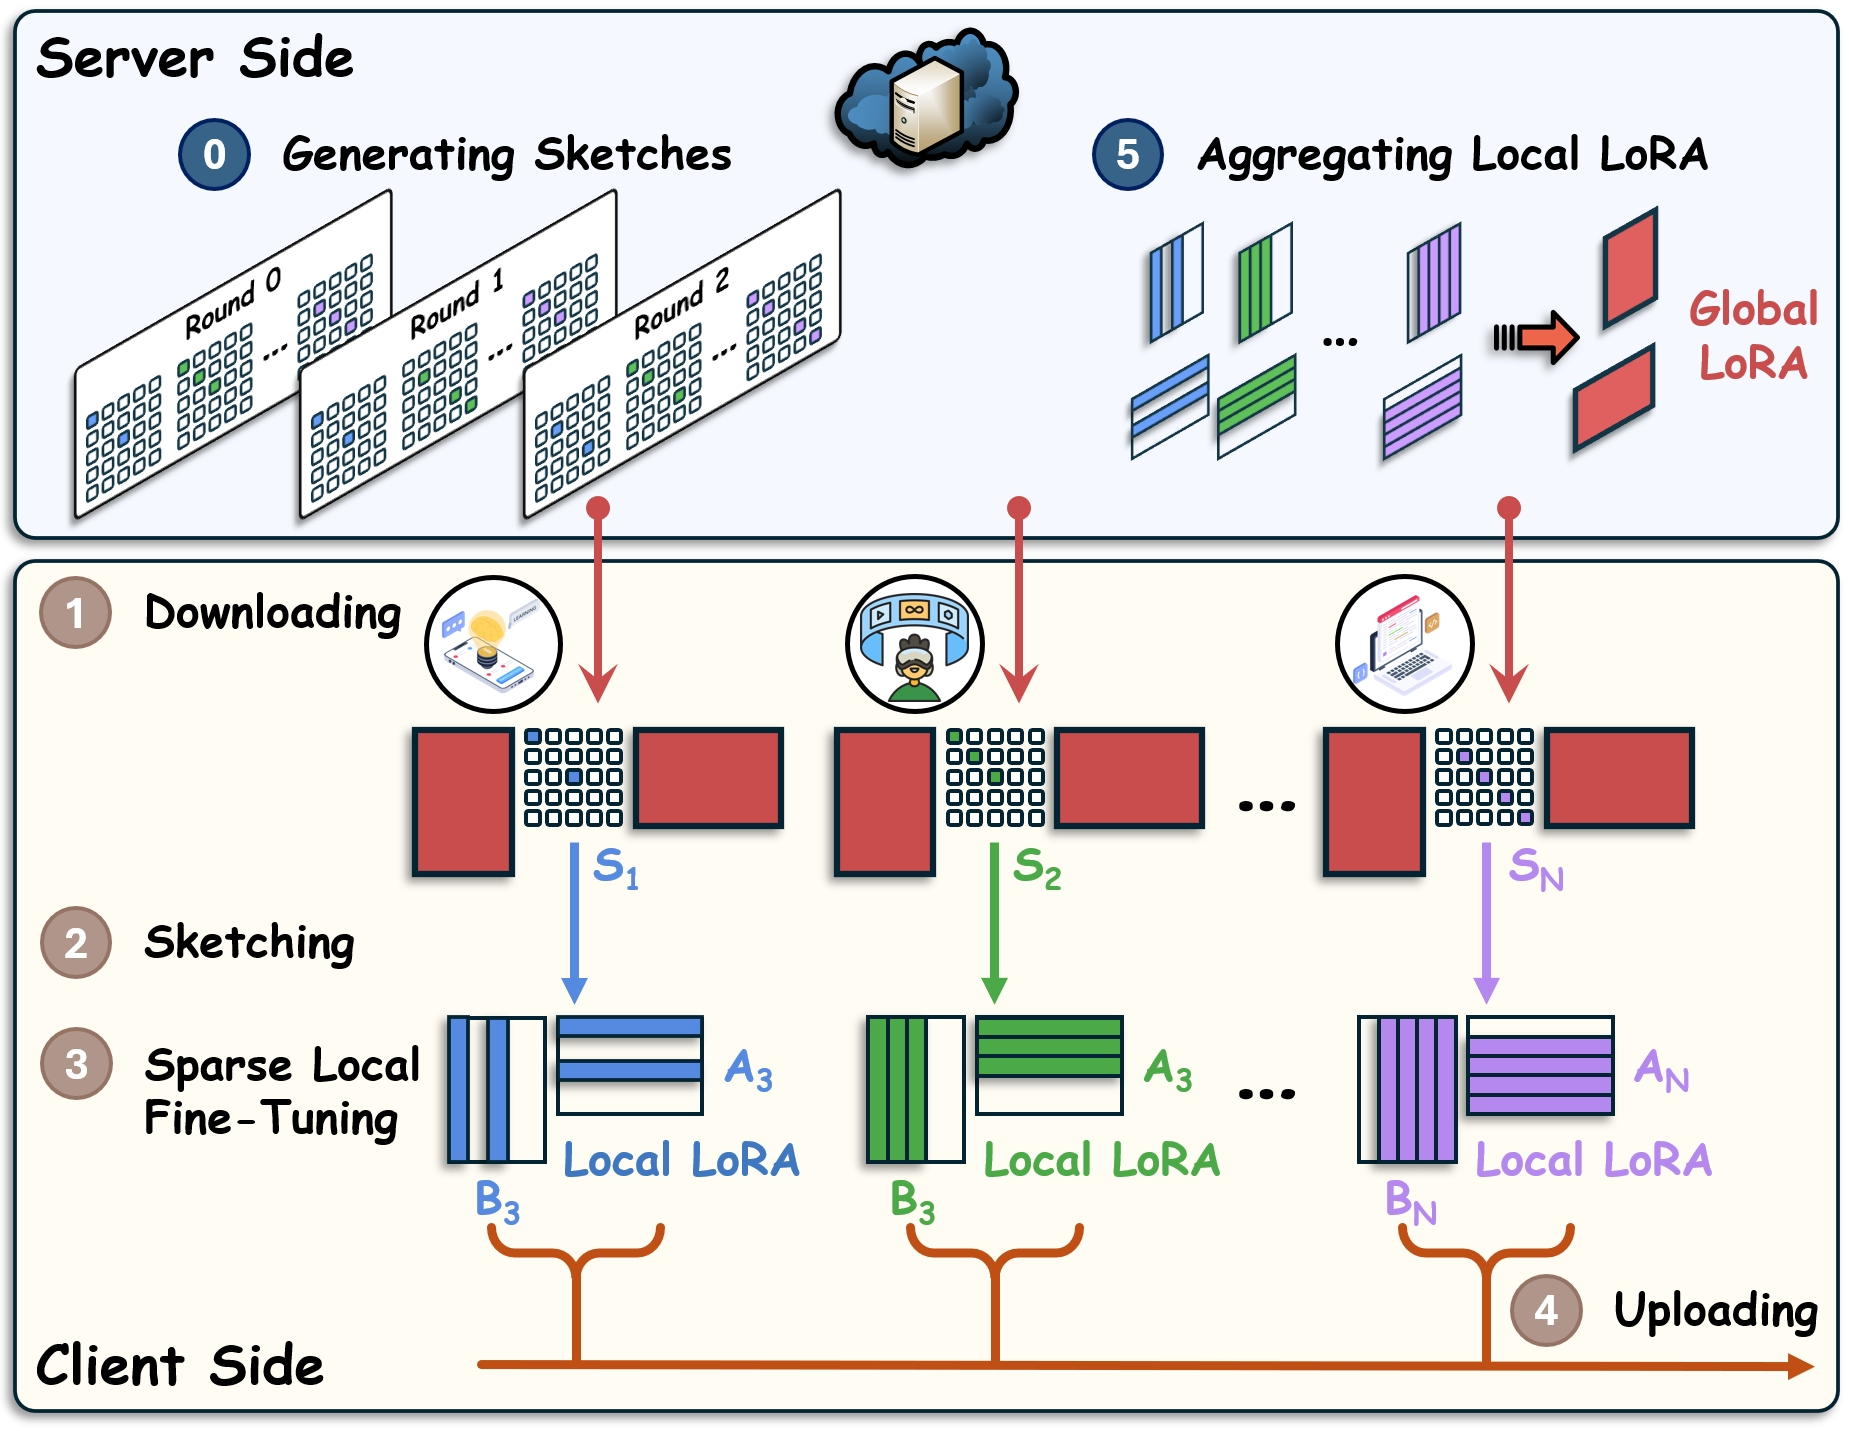
\includegraphics[width=\linewidth]{Figure/Overview.png}
    \caption{Overview}
    \label{fig:Overview}
\end{figure*}

\subsection{Our Formulation}
%Due to the heterogeneous federated learning system and resource-constrained network, forcing all the clients to update and upload the uniform-size $\bf{B}$ and $\bf{A}$ would be impractical. 
In this work, we proposed an alternative formulation for federated LoRA fine-tuning
\begin{equation}\label{lora_formulation_ours}
\begin{aligned}
\min_{\bf B,{\bf A}} f^{\mathcal{S}}(\bf B,{\bf A}) &\eqdef  \frac{1}{N} \sum_{i=1}^N f_i^{\mathcal{S}} (\bf B,{\bf A})\\
f_i^{\mathcal{S}}(\bf B,{\bf A}) &\eqdef  \mathbb{E}_{ {\bf S} \sim \mathcal{S}_i; \xi \sim \mathcal{D}_i} \left[ \ell ({\bf W}_{0} + {\bf B}\bf S{\bf A}, \xi)\right],
\end{aligned}
\end{equation}
where ${\bf W}_{0}$ denotes the pre-trained model, ${\bf B} \in \mathbb{R}^{m\times r},  {\bf A}\in \mathbb{R}^{r\times n}$ are LoRA modules, \(\ell\) is the sample-wise loss function, \(\mathcal{D}_i\) is the local dataset of client \(i\), and \(\mathcal{S}_i\) represents the sketching matrix set for client $i$. In addition, the random sketching matrix \(\bf S\) satisfies 
\begin{equation}
    \mathbb{E}[\mathbf{S}] = \mathbf{I}_r, \quad \text{and} \quad \mathbb{E}[\mathbf{S}^{\top} \mathbf{S}] \text{ is finite},
\end{equation}
where $\mathbf{I}_r$ is a $r$-dimensional identity matrix. Based upon this property, ${\bf W}_0 + {\bf B} {\bf S} {\bf A}$ can be treated as an unbiased estimate of ${\bf W}_0 + \bf B{\bf A}$. The proposed formulation, \eqref{lora_formulation_ours}, serves as an approximation of the original federated LoRA formulation, \eqref{fed_lora_formulation}. This approximation introduces greater flexibility for local fine-tuning on edge devices, as will be demonstrated in the following sections.
%We will characterize the bias between \eqref{fed_lora_formulation} and \eqref{lora_formulation_ours} in Section \ref{sec:analysis}.

\subsection{Sparsity in the Gradients}
In this subsection, we analyze the gradient structure of LoRA modules and highlight the sparsity properties of the gradients under our reformulation. To begin, we present the gradient expressions for the LoRA modules \(\bf B\) and \(\bf A\) with sketching matrix in the following lemma.
\begin{lemma}[Gradient Formulation]\label{compute_grad}
For a given sketching matrix \(\bf S\), the gradients of the loss function \(\ell(\bf W_0 + {\bf B}\bf S{\bf A}, \xi)\) with respect to ${\bf B}$ and ${\bf A}$ obey the following form
\begin{equation}\label{gradient_matrix}
\begin{aligned}
    {\nabla}_{\bf B} \tilde{\ell}(\bf B,{\bf A}, \xi) &= \nabla \ell({\bf W}_0 + {\bf B} {\bf S} {\bf A}, \xi)  {\bf A}^{\top} {\bf S}^{\top} \\
    {\nabla}_{\bf A} \tilde{\ell}(\bf B,{\bf A}, \xi) &= {\bf S}^{\top} {\bf B}^{\top} \nabla \ell(\bf W_0 + {\bf B}\bf S{\bf A}, \xi),
\end{aligned}
\end{equation}
where \({\nabla}_{\bf B} \tilde{\ell}(\bf B,{\bf A}, \xi)\), \({\nabla}_{\bf A} \tilde{\ell}(\bf B,{\bf A}, \xi)\), and \(\nabla \ell(\bf W_0 + {\bf B}\bf S{\bf A}, \xi)\) represent the gradient of \(\ell(\bf W_0 + {\bf B}\bf S{\bf A}, \xi)\) with respect to \(\bf B\), \(\bf A\), and \(\bf W_0 + {\bf B}\bf S{\bf A}\), respectively. 
\end{lemma}
\begin{proof}
    Following the chain rule $\nabla_{\bf Y} g({\bf X}{\bf Y}) ={\bf X}^{\top} \nabla g(\bf X{\bf Y}) $ and $\nabla_{\bf X} g(\bf X{\bf Y}) =  \nabla g({\bf X} {\bf Y}){\bf Y}^{\top}$, we can derive the gradients with respect to \(\bf B\) by setting \({\bf Y} = \bf S{\bf A}\) and \(\bf X = \bf B\). Similarly, we can obtain the gradients to \(\bf A\) by setting \(\bf X = {\bf B}\bf S\) and \({\bf Y} ={\bf A}\).
\end{proof}

Given the gradient expressions with sketching, we adopt the Random-$K$ diagonal matrix as the sketching matrix \(\mathbf{S}_i\). This choice enables edge devices to leverage the advantages of sparse training efficiently. 
The definition of the Random-$K$ diagonal sketching matrix, as introduced in \citep{demidovich2023mast}, is provided below:
\begin{definition}[Random-$K$ Sketching]\label{skeching_def}
A Random-$K$ diagonal sketching matrix is defined as:  
\[
\mathbf{S} = \frac{r}{K} \sum_{j \in \mathcal{I}} \mathbf{e}_j \mathbf{e}_j^\top,
\]  
where \(\mathbf{e}_1, \dots, \mathbf{e}_r \in \mathbb{R}^r\) are the standard unit basis vectors, and \(\mathcal{I}\) is a random subset of \([r]\), sampled uniformly from all subsets of \([r]\) with cardinality \(K\).  
\end{definition}

In particular, when $\bf S$ is a Random-$K$ diagonal sketching matrix, it can sample $K$ rows or columns of a matrix through left product or right product, respectively. In other words, when we enforce the sketching matrix $\bf S$ to be a Random-$K$ diagonal matrix, the gradients of $\ell({\bf W}_0 + {\bf B} {\bf S} {\bf A}, \xi)$ to LoRA modules \(\bf B\) and \(\bf A\) shown in \eqref{gradient_matrix} will be structural sparse matrices. 
\end{comment}

%Additionally, by setting different $K$ for different clients, we could support fine-tuning over a heterogeneous federated system. The aggregation of heterogeneous ranked updates will be introduced in the next Section \ref{sec:heterogeneous}.
\begin{comment}
\begin{remark}
Lemma \ref{compute_grad} aims to demonstrate the sparse structure of the gradients of the loss function \(\ell(\bf W_0 + {\bf B}\bf S{\bf A}, \xi)\) with respect to ${\bf B}$ and ${\bf A}$. However, this does not mean that we must compute the gradients directly through the chains shown in \eqref{gradient_matrix}. In fact, this is not how deep learning frameworks like PyTorch perform backpropagation. Otherwise, LoRA would suffer the same computational cost as full model fine-tuning, since the gradient \( \nabla \ell(\bf W_0 + {\bf B}\bf S{\bf A}, \xi) \) would have the same size as the full model. 
In practice, a lower-complexity chain is used to compute the gradients to the low-rank matrices \( \mathbf{B} \) and \( \mathbf{A} \). To illustrate, consider a model with one-layer forward pass: 
\(
\mathbf{h} = (\mathbf{W_0} + \mathbf{B} \mathbf{S} \mathbf{A}){\bf X},
\)
where \(\mathbf{h}\) is the prediction from this model for sample \(\xi = (\bf x, y)\), \(\bf x\) denotes the data and \(y\) is the label\footnote{For simplicity, we omit activations here.}. 
The loss \( \ell(\mathbf{W_0} + \mathbf{B} \mathbf{S} \mathbf{A}; \xi) \) can be expressed as:
\(
L\left((\mathbf{W_0} + \mathbf{B} \mathbf{S} \mathbf{A}){\bf X}, y_i\right),
\)
where \( L \) is the loss function applied to measure the bias between the prediction and label \( y \). The gradients with respect to \( \mathbf{B} \) and \( \mathbf{A} \) are
\(\nabla_{\mathbf{B}} \left( \nabla_{\mathbf{h}_i} \ell \right) \boldsymbol{\xi}_i^{\top} \mathbf{A}^{\top} \mathbf{S}^{\top}\) and
\(
\nabla_{\mathbf{A}} G_i^{\prime} = \mathbf{S}^{\top} \mathbf{B}^{\top} \left( \nabla_{\mathbf{h}_i} \ell \right) \boldsymbol{\xi}_i^{\top}.
\)
Mathematically, they will share the same results as shown in \eqref{gradient_matrix}.
In other words, we only need to compute the gradient with respect to the hidden state \( \mathbf{h} \), which is typically much smaller than the full-weight matrix. The gradients naturally flow through the hidden state to the low-rank matrices \( \mathbf{A} \) and \( \mathbf{B} \), ensuring efficient and scalable backpropagation. 
\end{remark}
\end{comment}

\section{Analysis} \label{sec:analysis}
%In this section, we analyze FSLoRA's convergence.  Our analysis relies on the following notations.
In this section, we analyze the convergence of the proposed FSLoRA algorithm. We show that the iterate sequence generated by the FSLoRA algorithm converges to a stationary point of the function \eqref{lora_formulation_ours}. Our analysis relies on the following notations.
 
\textbf{Notations:} We define \(\tilde{\ell} ({\bf B}, {\bf A}, \xi; {\bf S}) = \ell ({\bf W}_{0} + {\bf B} {\bf S} {\bf A}, \xi)\) and
\(\tilde{f}_{i} ({\bf B}, {\bf A}; {\bf S}) = \mathbb{E}_{\xi \sim \mathcal{D}_i} \left[ \ell ({\bf W}_{0} + {\bf B}\bf S{\bf A}, \xi)\right] \) for a given ${\bf S}$ 
%\[\tilde{f}_{i} ({\bf B}, {\bf A}; {\bf S}) = f_i({\bf B} {\bf S}, {\bf A}) \eqdef \mathbb{E}_{\xi \sim \mathcal{D}_i} \left[ \ell ({\bf W}_{0} + {\bf B}\bf S{\bf A}, \xi)\right]\]
and \( f_i^{\mathcal{S}}(\mathbf{B}, \mathbf{A}) = \mathbb{E}_{{\bf S} \sim \mathcal{S}_i} [\tilde{f}_{i} ({\bf B}, \mathbf{A}; {\bf S}) ] \). 
For simplicity, we denote \( \mathbf{X} = [\mathbf{B}; \mathbf{A}] \) and rewrite \( f(\mathbf{B}, \mathbf{A}) \), \( f_i(\mathbf{B}, \mathbf{A}) \), \( f^{\mathcal{S}}(\mathbf{B}, \mathbf{A}) \), \( f_i^{\mathcal{S}}(\mathbf{B}, \mathbf{A}) \), \( \tilde{f}_i({\bf B}, {\bf A}; {\bf S}) \), and \(\tilde{\ell} ({\bf B}, {\bf A}, \xi; {\bf S})\) as \( f(\mathbf{X}) \), \( f_i(\mathbf{X}) \), \( f^{\mathcal{S}}(\mathbf{X}) \), \( f_i^{\mathcal{S}}(\mathbf{X}) \), \( \tilde{f}_{i} (\mathbf{X}; \mathbf{S}) \), and \(\tilde{\ell} ({\bf X}, \xi; {\bf S})\) respectively. In addition, we use \(\|\cdot\|\) to denote the Frobenius norm.

We conduct analysis based on the following assumptions. 
\begin{assumption}\label{smoothness_assumption}
    \(f_i ({\bf X})\) is differentiable and \(L\)-smooth, i.e., there exists a positive constant \(L\) such that \(\forall {\bf X},{\bf Y}\),
    \[
    \|\nabla f_i({\bf X}) - \nabla f_i({\bf Y})\| \leq L \|{\bf X} - {\bf Y}\|, \forall i.
    \]
\end{assumption}
\begin{assumption}\label{varaince_assumption}
$\nabla_{\bf X}  \tilde{\ell} ({\bf X}, \xi; {\bf S}) $ is an unbiased estimate of $\nabla_{\bf X}  f_i^{\mathcal{S}} ({\bf X})$ and its variance is bounded as 
$$\mathbb{E}\| \nabla_{\bf X}  \tilde{\ell} ({\bf X}, \xi; {\bf S})  - \nabla_{\bf X}  f_i^{\mathcal{S}} ({\bf X})\|^2 \leq \rho \|\nabla_{\bf X}  f_i^{\mathcal{S}} ({\bf X})\|^2 +  \sigma^2, \forall i,$$
where the expectation is computed over $\xi \sim \mathcal{D}_i$ and ${\bf S}\sim \mathcal{S}_i$. 
\end{assumption}
\begin{assumption}\label{assumption:gradient_dissimilarity}
%There exist positive constants \(c_h\), \(\delta_h^2\) such that the gradient dissimilarity between the global loss and local loss can be bound as follows
The gradient dissimilarity between the global loss \(f^{\mathcal{S}}(\bf X)\) and each local loss \( f_i^{\mathcal{S}}(\bf X) \) satisfies
\begin{equation}
\left\| \nabla_{\bf X} f_i^{\mathcal{S}}({\bf X}) \!-\! \nabla_{\bf X} f^{\mathcal{S}}(\bf X) \right\|^2 \! \leq \! c_h \| \nabla_{\bf X} f^{\mathcal{S}}({\bf X}) \|^2  \!+\! \delta_h^2, \forall i, \nonumber
\end{equation}
where \(c_h \geq 0\) and \(f^{\mathcal{S}}(\mathbf{X}) = \frac{1}{N} \sum_{i=1}^N f_i^{\mathcal{S}}(\mathbf{X}) \).
\end{assumption}

Assumption \ref{smoothness_assumption} is standard in optimization literature \citep{bottou2018optimization,fang2024mtgc,bubeck2015convex}. Assumptions \ref{varaince_assumption} and \ref{assumption:gradient_dissimilarity} are commonly adopted in federated learning to bound sampling randomness and data heterogeneity  \citep{fang2022communication,yi2022zeroth}. 
We further provide an empirical validation in Appendix \ref{appen:justification_assumption}, showing that Assumptions \ref{varaince_assumption} and \ref{assumption:gradient_dissimilarity} are reasonable within the LLM fine-tuning scenario.
Building on these assumptions, we analyze the convergence behavior of FSLoRA. Our main results are summarized in the following theorem.
\begin{theorem}\label{convergence_fed_slora_condense}
    Suppose that Assumptions \ref{smoothness_assumption}-\ref{assumption:gradient_dissimilarity} hold, then there exists a learning rate $\gamma \leq \min \{\frac{N}{24 \rho (c_h + 1) H\bar{L}}, \frac{1}{8\sqrt{\widetilde{L} L (\rho+1) (c_h +1)} H}, \frac{1}{H} \}$ such that the iterates \(\{{\bf X}^t\}\) generated by FSLoRA satisfy 
\begin{align}
\frac{1}{T}\sum_{t=0}^{T-1} \!\mathbb{E} \left\| \nabla_{\bf X} f^{\mathcal{S}} ({\bf X}^t) \right\|^2 \! \leq \! 8 \frac{\sqrt{\bar{L} \mathcal{F}_0 \sigma_{\rho}^2} }{\sqrt{N TH}}
+ 10 (\widetilde{L} L)^{\frac{1}{3}} \left(\frac{\mathcal{F}_0 \sigma_{\rho}}{ T}\right)^{\frac{2}{3}} + \frac{4 \mathcal{F}_0 }{T},
\end{align}
where $ \sigma_{\rho}^2 = \sigma^2 + 3(\rho+1) \sigma_h^2$, \(\bar{L} = \left(\frac{1}{N} \sum_{i=1}^N \frac{r}{ k_i}\right) L \), \(\widetilde{L} = \left(\frac{1}{N} \sum_{i=1}^N \frac{r^2}{ k^2_i}\right) L\) and \(\mathcal{F}_0 = f^{\mathcal{S}}({\bf X}^0)  -  f^*\) with $f^*$ denoting the lower bound of $f^{\mathcal{S}}({\bf X})$.
\end{theorem}
\textbf{Technical highlights of Theorem \ref{convergence_fed_slora_condense}:}
A key step in the proof of Theorem \ref{convergence_fed_slora_condense} is characterizing the impact of the sketching mechanism on the optimization landscape. Our analysis reveals how the sketching operation modifies the smoothness properties of the objective, introducing scaled smoothness constants, $\frac{r}{k_i} L$ and $\frac{r^2}{k_i^2} L$, which directly influence the convergence behavior.
Further details are presented in Appendix \ref{proof_theorem}.  

\textbf{Discussion:} Theorem \ref{convergence_fed_slora_condense} establishes an upper bound on the convergence of the proposed FSLoRA algorithm. The parameters \(\bar{L}\) and \(\widetilde{L}\) provide insight into how the sketching operation influences the convergence rate. Increasing \(k_i\) would lead to a faster convergence for FSLoRA. However, this comes at the cost of increased communication and computational overhead for client $i$, indicating a trade-off in the selection of the sketching ratios. 
Additionally, the upper bound vanishes as $T \rightarrow \infty$. Moreover, the rate at which the bound diminishes is dominated by the first term, which recovers the convergence behavior of FedAvg \citep{yu2019parallel,khaled2020tighter,karimireddy2020scaffold} as the sketching ratio $k_i/r \to 1$(i.e., $\bar{L} = L$). This highlights the tightness of our analysis and shows that FSLoRA retains the convergence guarantees of vanilla Federated LoRA in the limit.
\begin{comment}
delete for ICLR submission for condensing the content
\begin{theorem}\label{convergence_fed_slora}
    Suppose that Assumptions \ref{smoothness_assumption}-\ref{assumption:gradient_dissimilarity} hold and the learning rate satisfies $\gamma \leq \min \{\frac{N}{24 \rho (c_h + 1) H\bar{L}}, \frac{1}{8\sqrt{\widetilde{L} L (\rho+1) (c_h +1)} H} \}$. Then the iterates \(\{{\bf X}^t\}_{t=0}^{T-1}\) generated by FSLoRA satisfy 
\begin{align}
 \frac{1}{T} \sum_{t=0}^{T-1} \!\mathbb{E}  \left\| \nabla_{\bf X} f^{\mathcal{S}} ({\bf X}^t) \right\|^2  \leq  4 \frac{f^{\mathcal{S}}({\bf X}^0)  -  f^*}{\gamma TH} + \gamma \frac{4 \bar{L}}{N} \sigma_{\rho}^2 \!+\! 10 \gamma^2 H^2 \widetilde{L} L \sigma_{\rho}^2,
\end{align}
where $ \sigma_{\rho}^2 = \sigma^2 + 3(\rho+1) \sigma_h^2$, \(\bar{L} = \left(\frac{1}{N} \sum_{i=1}^N \frac{r}{ k_i}\right) L \), \(\widetilde{L} = \left(\frac{1}{N} \sum_{i=1}^N \frac{r^2}{ k^2_i}\right) L\), and $f^*$ denotes the lower bound of $f^{\mathcal{S}}({\bf X})$.
\end{theorem}

\textbf{Technical highlights of Theorem \ref{convergence_fed_slora}:}
A key step in the proof of Theorem \ref{convergence_fed_slora} is characterizing the impact of sketching mechanism on the optimization landscape. Our analysis reveals how the sketching operation modifies the smoothness properties of the objective, introducing scaled smoothness constants, $\frac{r}{k_i} L$ and $\frac{r^2}{k_i^2} L$, which directly influence the convergence behavior.
Further details are presented in Appendix \ref{proof_theorem}.  


Based on the results in Theorem \ref{convergence_fed_slora}, we obtain the following corollary by applying an appropriate learning rate \(\gamma\) to Algorithm \ref{alo_flora}. The proof can be found in Appendix \ref{proof_coro}. 

\begin{corollary}\label{coro_convergence_fed_slora}
Under the same assumptions of Theorem \ref{convergence_fed_slora}, let \(\mathcal{F}_0 = f^{\mathcal{S}}({\bf X}^0)  -  f^*\). Then there exists a learning rate \(\gamma\) meeting the condition outlined in Theorem \ref{convergence_fed_slora} such that the iterates \(\{{\bf X}^t\}_{t=0}^{T-1}\) generated by FSLoRA satisfy
\begin{align}
\frac{1}{T}\sum_{t=0}^{T-1} \!\mathbb{E} \left\| \nabla_{\bf X} f^{\mathcal{S}} ({\bf X}^t) \right\|^2 \! \leq \! 8 \frac{\sqrt{\bar{L} \mathcal{F}_0 \sigma_{\rho}^2} }{\sqrt{N TH}}
+ 10 (\widetilde{L} L)^{\frac{1}{3}} \left(\frac{\mathcal{F}_0 \sigma_{\rho}}{ T}\right)^{\frac{2}{3}} + \frac{4 \mathcal{F}_0 }{T}.
\end{align}
\end{corollary}
\textbf{Discussion:} Corollary \ref{coro_convergence_fed_slora} establishes an upper bound on the convergence of the proposed FSLoRA algorithm. The parameters \(\bar{L}\) and \(\widetilde{L}\) provide insight into how the sketching operation influences the convergence rate. Increasing \(k_i\) would lead to a faster convergence for FSLoRA. However, this comes at the cost of increased communication and computational overhead for client $i$, indicating a trade-off in the selection of the sketching ratios. 
Additionally, the upper bound vanishes as $T \rightarrow \infty$. Moreover, the rate at which the bound diminishes is dominated by the first term, which recovers the convergence behavior of FedAvg \citep{yu2019parallel,khaled2020tighter,karimireddy2020scaffold} as the sketching ratio $k_i/r \to 1$(i.e., $\bar{L} = L$). This highlights the tightness of our analysis and shows that FSLoRA retains the convergence guarantees of vanilla Federated LoRA in the limit.
\end{comment}


\begin{comment}
The results obtained in Corollary \ref{coro_convergence_fed_slora} show the impacts of the variance associated with the stochastic gradient (i.e., \(\sigma^2\)) and the data heterogeneity (i.e., \(\sigma_h^2\)) on FSLoRA's convergence. Furthermore, the parameters \(\bar{L}\) and \(\widetilde{L}\) provide insight into how the sketching operation influences the convergence rate. 
%Specifically, it scales the smoothness constant \(L\) by the average the squared sketching factor across all devices, given by \(\frac{1}{N} \sum_{i=1}^N \frac{r}{k_i}\). 
Increasing \(k_i\) would lead to a faster convergence rate for FSLoRA. However, on the other hand, as \(k_i\) increases, the communication and computation costs at device \(i\) will increase. In other words, there is a trade-off in the selection of the sketching ratios. 
Additionally, Corollary \ref{coro_convergence_fed_slora} suggests that FSLoRA achieves a similar linear speedup in the number of local updates and the number of devices as FedAvg \citep{yu2019parallel,khaled2020tighter}.
\end{comment}

\begin{comment}
\begin{remark}
In this work, we utilize the sketching formulation to reformulate the fine-tuning problem as \eqref{lora_formulation_ours}, which can be treated as an approximation of the original LoRA fine-tuning problem. When the sketches are identity matrices, these two formulations are equivalent. In addition, for general cases, we can bound the approximation error, which is summarized in the following proposition.
\begin{proposition}\label{approximation_error}
The approximation error between \(f^{\mathcal{S}}(\mathbf{X})\) and \(f(\mathbf{X})\) can be bounded as follows.
    \begin{itemize}
        \item If the loss function \(\ell (\bf W, \xi)\) is linear with respect to $\bf W$, then \(f^{\mathcal{S}}(\mathbf{X}) =f(\mathbf{X})\).
        %\item If the loss function $\ell (\bf W)$ is convex, then \(f^{\mathcal{S}}(\mathbf{X}) \geq f(\mathbf{X})\)
        %\item If the loss function $\ell (\bf W)$ is $L_0$-smooth, then \(f^{\mathcal{S}}(\mathbf{X}) \leq f(\mathbf{X}) + \frac{L_0}{2} \left(\frac{r^2}{\min k_i^2} - 1\right)\|X\|^2\)
        \item If the loss function $\ell ({\bf W}, \xi)$ is convex and \(L\)-smooth, then
        \[0 \leq f^{\mathcal{S}}(\mathbf{X}) -f(\mathbf{X}) \leq \frac{L}{2} \left(\frac{r}{\min k_i} - 1\right)\|{\bf B}\|^2 \|{\bf A}\|^2,\] where \( \mathbf{X} = [\mathbf{B}; \mathbf{A}] \).
    \end{itemize}
\end{proposition}
\noindent The proof details are provided in Appendix \ref{prove_proposition_error}. It is worth mentioning that the convexity assumption is usually made to characterize the function value relationship, as the function value of a non-convex function is typically hard to analyze. Proposition \ref{approximation_error} aims to show the bias between the function values of \( f^{\mathcal{S}}(\mathbf{X}) \) and \( f(\mathbf{X}) \).
\end{remark}
\end{comment}


\section{Experiments}\label{sec:experiment}
\counterwithin{table}{section}
\newcommand{\com}[1]{\tiny$\pm$#1}

\begin{table}[t]
\caption{
Testing accuracy over 3 independent runs on GLUE and commonsense reasoning benchmarks. 
FSLoRA achieves a notable improvement in average performance compared to the baselines.
}
\centering
\small
\resizebox{\linewidth}{!}{
\begin{tabular}{l|c|ccccccc|c}
\multicolumn{10}{c}{\textbf{GLUE benchmark (RoBERTa model)}} \\
\toprule
Method  & GPU hours & QNLI & MRPC & CoLA & MNLI & RTE & SST-2 & QQP & Avg. \\
\midrule
HeteroLoRA & 10.7h & 87.5 \com{0.5} & 84.4 \com{0.9} & 75.3 \com{1.2} & 66.3 \com{0.8} & 69.0 \com{1.7} & 89.5 \com{0.0} & 85.3 \com{0.1} & 79.6  \\
FlexLoRA & 12.6h & 88.5 \com{0.2} & 81.2 \com{0.4} & 77.5 \com{1.2} & 63.0 \com{0.5} & 62.2 \com{1.9} & 92.8 \com{0.4} & 87.4 \com{0.1} & 78.9  \\
FLoRA & 12.3h & 87.2 \com{0.3} & 78.1 \com{0.7} & 77.4 \com{1.7} & 74.6 \com{0.5} & 54.4 \com{2.1} & 93.4 \com{0.1} & 87.1 \com{0.3} & 78.9  \\
\rowcolor{ours} FSLoRA & 10.9h & 88.0 \com{0.3} & 87.3 \com{0.2} & 82.2 \com{0.5} & 76.4 \com{0.2} & 69.8 \com{1.2} & 93.5 \com{0.1} & 85.8 \com{0.1} & 83.3  \\
\midrule
\end{tabular}
}

%\vspace{1mm}

\resizebox{\linewidth}{!}{
\begin{tabular}{l|c|cccccccc|c}
\multicolumn{11}{c}{\textbf{Commonsense reasoning benchmark (LLaMA-3.2-3B model)}} \\
\toprule
Method & GPU hours & ARC-c & ARC-e & BoolQ & HellaSwag & OBQA & PIQA & SIQA & WinoGrande & Avg. \\
\midrule
HeteroLoRA & 43.7h & 73.4 \com{0.3} & 86.6 \com{0.2} & 65.8 \com{0.5} & 73.0 \com{0.5} & 71.4 \com{0.3} & 80.9 \com{0.7} & 73.8 \com{0.3} & 72.0 \com{0.3} & 74.6 \\
FlexLoRA & 68.3h & 74.2 \com{0.3} & 86.7 \com{0.6} & 68.6 \com{0.8} & 79.4 \com{0.7} & 75.8 \com{0.4} & 81.0 \com{0.3} & 75.9 \com{0.4} & 77.9 \com{0.3} & 77.4 \\
FLoRA & 49.8h & 68.3 \com{0.6} & 83.1 \com{0.5} & 65.8 \com{0.9} & 77.2 \com{0.5} & 74.2 \com{0.3} & 80.5 \com{0.6} & 76.1 \com{0.5} & 71.5 \com{0.5} & 74.6 \\
%\rowcolor{ours} FSLoRA & 44.5h & 73.8 \com{0.6} & 86.2 \com{0.1} & 68.5 \com{0.1} & 83.1 \com{1.1} & 78.7 \com{0.3} & 82.0 \com{0.2} & 75.8 \com{0.0} & 74.8 \com{0.6} & 77.9 \\
\rowcolor{ours} FSLoRA & 44.3h & 76.1 \com{0.4} & 87.2 \com{0.5} & 69.3 \com{0.7} & 82.2 \com{1.1} & 80.7 \com{0.6} & 84.0 \com{0.2} & 76.8 \com{0.0} & 79.1 \com{0.2} & 79.4 \\
\bottomrule
\end{tabular}
}
\label{tab:combined_vertical}
\vspace{-4mm}
\end{table}


\begin{comment}
\begin{table*}[h]
%\vspace{-2mm}
\caption{Testing accuracy over 3 independent runs for fine-tuning the RoBERTa model on the GLUE benchmark. 
%The computational time for our experiments is reported in GPU hours.
%For FSLoRA, the rank of global LoRA modules is fixed at $r=64$ while the sketching ratio for each device \(\frac{k_i}{r}\) is independently sampled from \(\{0.125, 0.25, 0.5, 0.75\}\). For a fair comparison, the ranks of local LoRA modules for devices are sampled from $\{8, 16, 32, 48 \}$.
FSLoRA achieves a notable improvement in average performance compared to the baselines.
}
\vspace{-1mm}
\small
\centering
\resizebox{\linewidth}{!}{
\begin{tabular}{l|c|ccccccc|c}
\toprule
Method  & GPU hours & QNLI & MRPC & CoLA & MNLI & RTE &  SST-2  & QQP  & Avg. \\
\midrule
HeteroLoRA & 10.7h & 87.5 \com{0.5} & 84.4 \com{0.9} & 75.3 \com{1.2} & 66.3 \com{0.8} & 69.0 \com{1.7} & 89.5 \com{0.0} & 85.3 \com{0.1} & 79.6  \\
FlexLoRA & 12.6h & 88.5 \com{0.2} & 81.2 \com{0.4} & 77.5 \com{1.2} & 63.0 \com{0.5} & 62.2  \com{1.9} & 92.8  \com{0.4} & 87.4  \com{0.1} & 78.9  \\
FLoRA & 12.3h & 87.2 \com{0.3} & 78.1 \com{0.7} & 77.4  \com{1.7} & 74.6 \com{0.5} & 54.4 \com{2.1} & 93.4  \com{0.1} & 87.1  \com{0.3} & 78.9  \\
\midrule
\rowcolor{ours} FSLoRA & 10.9h & 88.0 \com{0.3} & 87.3  \com{0.2} & 82.2 \com{0.5} & 76.4  \com{0.2} & 69.8 \com{1.2} & 93.5 \com{0.1} & 85.8 \com{0.1} & 83.3  \\
\bottomrule
\end{tabular}
}
\label{tab:robert_het_accuracy}
%\vspace{-4mm}
\end{table*}


\begin{table*}[t]
\caption{
Testing accuracy over 3 independent runs for fine-tuning the LLaMA-3.2-3B model on the commonsense reasoning benchmark.
% , where Params refers to the number of trainable parameters while Commun represents the minimum uploading communication cost among edge devices. 
%The LoRA rank and sketching ratio setups are the same as those of Table \ref{tab:robert_het_accuracy}. 
FSLoRA demonstrates consistent performance improvement across these tasks compared to baselines.
}
\label{tab:llama_het_accuracy}
\vspace{-1mm}
\centering
%\tableindent 
\resizebox{\linewidth}{!}{
\begin{tabular}{l|c|cccccccc|c}
    \toprule
    Method & GPU hours & ARC-c & ARC-e & BoolQ & HellaSwag & OBQA & PIQA & SIQA & WinoGrande & Avg. \\
    \midrule
    HeteroLoRA & 44.2h & 69.2 \com{0.2} & 84.6 \com{0.2} & 68.4 \com{0.5} & 80.0 \com{0.7} & 69.9 \com{0.0} & 77.3 \com{0.0} & 68.7 \com{0.3} & 72.0 \com{0.3} & 73.8 \\
    FlexLoRA & 60.8h & 69.9 \com{0.3} & 84.7 \com{0.4} & 66.9 \com{0.2} & 80.5 \com{0.4} &  72.3\com{0.1} & 78.1\com{0.2} & 70.4 \com{0.4} & 73.3 \com{0.5} & 74.5 \\
    FLoRA & 56.2h & 67.5 \com{0.7} & 83.1 \com{0.5} & 65.8 \com{0.9} & 78.4 \com{0.5} & 69.2\com{0.7} & 75.5 \com{0.6} & 67.1 \com{0.3} & 71.5 \com{0.5} & 72.3 \\
    \midrule
    \rowcolor{ours} FSLoRA & 44.5h & 73.8 \com{0.6} & 86.2 \com{0.1} & 68.5 \com{0.1} & 83.1 \com{1.1} & 78.7 \com{0.3} & 82.0 \com{0.2} & 75.8 \com{0.0} & 74.8 \com{0.6} & 77.9 \\
    \bottomrule
\end{tabular}
}
\end{table*}
\end{comment}


%In this section, we present experiments to evaluate the performance of the proposed FSLoRA. All the experiments are conducted on a cluster equipped with 4 NVIDIA A100 GPUs, each with 40 GB of memory. \textcolor{blue}{The number of devices is set to \(20\) in the main experiments.} Other hyperparameter configurations can be found in Appendix \ref{appen:hyperparameters}. %The code for this project is available at \url{https://anonymous.4open.science/r/Federated-Sketching-LoRA}.
\begin{comment}
In this section, we present experiments to evaluate the performance of the proposed FSLoRA algorithm. 
In the main results, we consider the \textcolor{blue}{heterogeneous LoRA scenario} and compare the performance achieved by our approach with three established baselines designed for collaborative fine-tuning on resource-heterogeneous devices, i.e., HeteroLoRA \citep{cho2024heterogeneouslorafederatedfinetuning}, FlexLoRA \citep{bai2024federatedfinetuninglargelanguage}, and FLoRA \citep{wang2024flora}.
In the ablation study, we first investigate the efficiency advantage of FSLoRA by comparing the results attained by the proposed approach with those of the vanilla Federated LoRA under the same rank (i.e., \(r\)) and the same communication budget. 
Subsequently, we fix the rank of submatrices updated by the devices (i.e., \(k_i\)) and study the impact of the rank of global LoRA modules (i.e., \(r\)) on the performance of FSLoRA.
Finally, we fix the rank of global LoRA modules (i.e., \(r\)) and  \textcolor{blue}{investigate how the sketching ratio \(k_i/r\)} impacts the performance of FLoRA.
%Notably, in our experiments, we replace the original LoRA with rank-stabilized LoRA \citep{kalajdzievski2023rankstabilizationscalingfactor} for all methods for a more stable performance.
%including the baselines, to ensure consistent and improved performance as the rank increases. 
All the experiments are conducted based on a cluster of $4$ NVIDIA A100 GPUs with $40$ GB memory. Details about hyperparameter configurations are provided in Appendix \ref{appen:hyperparameters}. The code for this project is available at \url{https://anonymous.4open.science/r/Federated-Sketching-LoRA}
\end{comment}


%\textbf{Models, datasets, hyperparameters, and compute setting:} 

%\subsection{Experiment Setup}
%\textbf{Setup:} 
%Our experiments mainly focus on RoBERTa (125M) \citep{liu2019roberta} and LLaMA-3.2-3B (3.21B) \citep{llama3}, which reflect the typical scale of models suitable for on-device deployment.For RoBERTa and LLaMA-3.2-3B models, we fine-tune and evaluate them on the GLUE \citep{wang2018glue} and commonsense reasoning benchmark \citep{hu2023llm}, respectively. \textcolor{red}{Additionally, we extend our evaluation to the LLaMA-7B model in Appendix \ref{appen:larger_model}.
Our experiments focus on RoBERTa (125M) \citep{liu2019roberta} and LLaMA-3.2-3B \citep{llama3}, which represent typical model sizes suitable for client-side deployment, as well as the LLaMA-7B model to reflect large-scale scenarios.
For RoBERTa and LLaMA-3.2-3B models, we fine-tune and evaluate them on the GLUE \citep{wang2018glue} and commonsense reasoning benchmark \citep{hu2023llm}, respectively. For the LLaMA-7B model, we utilize Wizard, Dolly-15k, and Alpaca datasets, where the results are reported in Appendix \ref{appen:larger_model}.
Similar to \citep{zhang2024towards,wang2024flora}, we adopt Dirichlet-based partitioning for dataset splits.
%Further details on these datasets are provided in the Appendix \ref{appen:benchmarks}. 
All the experiments are conducted on a cluster equipped with 4 NVIDIA A100 GPUs, each with 40 GB of memory. The number of clients is set to $20$ in the main manuscript, and to $50$ and $100$ in Appendix \ref{appen:broader_heterogeneity}.
%Other hyperparameter configurations can be found in Appendix \ref{appen:hyperparameters}. 
Further details are provided in the Appendix \ref{appen:implementation_details}. 
%The code is available at \url{https://anonymous.4open.science/r/Federated-Sketching-LoRA-Implementation} and included in the supplementary material.
The implementation code for this project is included in the supplementary material.


\begin{comment}
\textbf{Models and Datasets:} Our experiments are mainly based on the RoBERTa model \citep{liu2019roberta}, a transformer-based architecture that serves as a robustly optimized version of BERT. It leverages a larger pretraining corpus and dynamic masking techniques, enhancing its performance on a wide range of NLP tasks. We load the pre-trained RoBERTa base (125M) from the Huggingface transformer library and fine-tune it on GLUE benchmark, including QNLI, MRPC, CoLA, MNLI, RTE, SST-2, and QQP tasks.
%Question-Answering Natural Language Inference (QNLI), Microsoft Research Paraphrase Corpus (MRPC), Corpus of Linguistic Acceptability (CoLA), MNLI (Multi-Genre Natural Language Inference), Stanford Sentiment Treebank (SST-2), and Quora Question Pairs (QQP). %Specifically, we apply LoRA to the key and query components in attention layers as well as the output linear layer, optimizing the model's ability to learn task-specific representations. 
Additionally, we scale up the model to LLaMA-3.2-3B for a commonsense reasoning task using the Commonsense170K dataset \citep{hu2023llm}. Specifically, we fine-tune the pretrained LLaMA-3.2-3B model (available on Hugging Face) with about 170K training samples constructed by \citep{hu2023llm}. The fine-tuned model is then evaluated on eight commonsense reasoning question-answering benchmarks, including BoolQ, PIQA, SIQA, HellaSwag, WinoGrande, ARC-c, ARC-e, and OBQA. Notably, the Commonsense170K dataset combines the training sets of these benchmarks into a unified corpus. The details about all the benchmarks considered in this work are provided in Appendix \ref{appen:benchmarks}. 
\end{comment}

%\textbf{Models and Datasets:} 
%Our experiments are mainly based on the RoBERTa base model (125M) \citep{liu2019roberta}, a robustly optimized version of BERT \citep{devlin2018bert}, and LLaMA-3.2-3B \citep{llama3}, which are based on the encoder-decoder and decoder-only transformer architectures, respectively. For the former, we load the pre-trained RoBERTa model from the Huggingface and fine-tune it on the GLUE benchmark \citep{wang2018glue}, including QNLI, MRPC, CoLA, MNLI, RTE, SST-2, and QQP tasks. For the latter, we fine-tune the pre-trained LLaMA-3.2-3B model, available on Hugging Face as well, for a commonsense reasoning task using the Commonsense170K dataset \citep{hu2023llm}. The fine-tuned model is then evaluated on eight commonsense reasoning question-answering benchmarks, including ARC-c, ARC-e, BoolQ, HellaSwag, OBQA, PIQA, SIQA, and WinoGrande. %Notably, the Commonsense170K dataset combines the training sets of these benchmarks into a unified corpus. Details about these datasets are provided in Appendix \ref{appen:benchmarks}. 

%\textbf{FL Settings:} We set the number of edge devices as $20$. Each device performs $H=20$ local training steps per communication round before aggregating updates. The data is distributed among devices using a Dirichlet distribution with a concentration parameter of $0.1$. This aims to introduce heterogeneity in the data across devices, reflecting real-world FL scenarios where data is often non-independent and identically distributed (Non-IID). 

%\subsection{Heterogeneous Rank Case}

%\subsection{Main Results}
%\subsection{Results and Discussion}
%\textbf{Baselines for Heterogeneous LoRA Settings:} We consider the following state-of-the-art baselines that integrate LoRA with FL: HeteroLoRA \citep{cho2024heterogeneouslorafederatedfinetuning}, FlexLoRA \citep{bai2024federatedfinetuninglargelanguage}, and FLoRA \citep{wang2024flora}. In our approach, the rank of the global LoRA modules is fixed as $r=64$, while the sketching ratio for device $i$ is sampled from the set $\{0.125, 0.25, 0.5, 0.75\}$. To ensure a fair comparison, we apply the same rank configuration to all baseline methods.

\subsection{Main Results Under Heterogeneous LoRA Setup}

\textbf{Performance comparison with baselines:} 
%We consider the following state-of-the-art baselines that integrate LoRA with FL: HeteroLoRA \citep{cho2024heterogeneouslorafederatedfinetuning}, FlexLoRA \citep{bai2024federatedfinetuninglargelanguage}, and FLoRA \citep{wang2024flora}. 
We consider three state-of-the-art baselines listed in Section \ref{sec:limitations_of_existing}.
For FSLoRA, the rank of the global LoRA modules is fixed as $r=64$, while the sketching ratio for client $i$ is sampled from the set $\{0.125, 0.25, 0.5, 0.75\}$. For a fair comparison, we apply the same rank configuration to all baseline methods. 
%Table \ref{tab:combined_vertical} presents the performance of FSLoRA and baseline methods on two benchmarks: the GLUE benchmark using the RoBERTa model and the commonsense reasoning benchmark using the LLaMA-3.2-3B model.
Table \ref{tab:combined_vertical} presents the performance of FSLoRA and baseline methods.
Across both settings, FSLoRA consistently achieves superior accuracy while maintaining low GPU hours. In the GLUE \& RoBERTa task, FSLoRA outperforms all baselines on average, with significant gains in MRPC, CoLA, and MNLI. In the commonsense reasoning \& LLaMA task, which introduces higher model complexity, FSLoRA also delivers the best overall performance. 
%Notably, FSLoRA achieves this while preserving computational efficiency comparable to HeteroLoRA, and substantially lower than FlexLoRA and FLoRA, as reflected in GPU hours. 
Notably, FSLoRA achieves this while preserving computational efficiency comparable to HeteroLoRA as reflected in GPU hours.
These results highlight FSLoRA's effectiveness and scalability in heterogeneous LoRA fine-tuning scenarios.

% \textbf{Evaluation under Broader Heterogeneity:} In Appendix \ref{}, we extend our evaluation to $50$ devices, incorporating greater diversity in clients’ communication and computation capabilities, as well as increased data heterogeneity.

% \textbf{Experiments with Larger Model:} In Appendix \ref{}, we compared our methods with baselines with LLaMA-7B model. 


\textbf{Evaluation under broader heterogeneity, increased number of clients, and larger model:} In Appendix \ref{appen:broader_heterogeneity}, we extend our evaluation to $50$ and $100$ clients, incorporating greater diversity in clients' communication and computation capabilities, as well as varying levels of data heterogeneity. In Appendix \ref{appen:larger_model}, we further assess the effectiveness of our method on the LLaMA-7B model.

\begin{comment} May 1
\textbf{RoBERTa Model:} Table \ref{tab:robert_het_accuracy} presents a performance comparison between the proposed FSLoRA and baseline methods in the heterogeneous LoRA scenario on the GLUE benchmark with the RoBERTa model. 
%In our approach, the rank of the \textcolor{blue}{global LoRA modules} is fixed at $r=64$, while the sketching ratio for device $i$ is sampled from $\{0.125, 0.25, 0.5, 0.75\}$. For a fair comparison, the ranks of local LoRA modules for devices in the baseline methods are accordingly sampled from the set $\{8, 16, 32, 48\}$.
%%%%%
As shown in Table \ref{tab:robert_het_accuracy}, compared with the baselines, our approach boosts the average performance across these seven tasks by a noticeable margin. Concretely, FSLoRA consistently outperforms HeteroLoRA across all the considered tasks. 
%It is worth noting that FSLoRA and HeteroLoRA share a similar level of simplicity in computation and communication complexity. This highlights that our approach not only retains the ease and efficiency of HeteroLoRA but also achieves superior performance.
%%%%%%
In addition, our approach significantly outperforms FlexLoRA in most tasks, with marginal performance differences only in QNLI and QQP. Similarly, it outperforms FLoRA on all tasks with the exception of the QQP task. 
%Importantly, our method achieves these results without the additional communication and computational overhead required by both FlexLoRA and FLoRA. 
%Importantly, FSLoRA and HeteroLoRA share a similar level of simplicity in computation and communication complexity, while FlexLoRA incurs additional server-side computational costs by performing SVD operations in every communication round and FLoRA similarly increases overhead by transmitting large concatenated matrices to edge devices, which must then compute and integrate the product $\bf BA$ into the frozen model each round, resulting in both higher communication costs and computational burden on the edge devices. 
It is worth noting that FSLoRA and HeteroLoRA maintain similar simplicity in computation and communication complexity, whereas FlexLoRA and FLoRA incur additional overhead, as detailed in Section \ref{sec:limitations_of_existing}. This increased computational complexity is also reflected in GPU hours, which represent the total computational time accumulated across all devices. As reported in Table \ref{tab:robert_het_accuracy}, FSLoRA and HeteroLoRA demonstrate comparable computational efficiency, requiring similar GPU hours, whereas FlexLoRA and FLoRA incur higher computational costs.
\end{comment}

%These additional complexities are also reflected in GPU hours.
%\textcolor{blue}{This is reflected in the GPU hours, which represent the total computational time accumulated across all devices.}
%The computational time for our experiments is reported in GPU hours, providing an accurate measure of resource utilization.

%Concretely, FlexLoRA introduces additional computational overhead on the server side by requiring SVD on the aggregated matrix during every communication round. Similarly, FLoRA adds significant communication overhead by transmitting large concatenated matrices to edge devices, which also increases the computational burden on the devices as they must integrate the resulting product $\bf BA$ into the frozen model in each round. These added complexities make both approaches less efficient in terms of communication and computation compared to simpler alternatives.

\begin{comment}
 In Figure \ref{fig:convergence}, we present the averaged testing accuracy of the proposed algorithm alongside the baseline methods across seven tasks described in Section \ref{sec:model_dataset}, plotted against the communication rounds, showcasing the convergence behavior of the proposed algorithm. FlexLoRA achieves fast initial convergence but falls behind in final accuracy due to the approximation errors introduced by its use of truncated SVD, which is effective early on but limits long-term performance. Similarly, HeteroLoRA's reliance on zero-padding reduces optimization efficiency, preventing it from achieving higher accuracy. FLoRA also underperforms due to the random reinitialization of LoRA modules at each communication round, disrupting tuning continuity. In contrast, FSLoRA overcomes these limitations, achieving the highest final accuracy among all methods.

 \begin{figure}[h]
    \centering
    \includegraphics[width=0.85\linewidth]{Figure/Results_RoBERTa.png}
    \vskip -0.05in
    \caption{Convergence behavior of FSLoRA and baselines on the GLUE benchmark with the RoBERTa model. Testing accuracy is averaged over seven tasks.}
    \label{fig:convergence}
    \vskip -0.05in
\end{figure}
\end{comment}

\begin{comment} May 1
\textbf{LLaMA-3.2-3B Model:} 
In Table \ref{tab:llama_het_accuracy}, we scale up to LLaMA-3.2-3B, which contains \(3.21\) billion parameters, to evaluate the effectiveness of our proposed algorithm with increasing model complexity.
The experimental results demonstrate that FSLoRA consistently achieves superior performance compared to baseline methods across all benchmark tasks. 
This advantage is particularly significant because fine-tuning LLaMA-3.2-3B, with its substantially larger parameter count, introduces greater challenges for deployment on heterogeneous distributed devices with limited computational and communication resources.
This further demonstrates the superiority of the proposed FSLoRA.
\end{comment}


%The most significant improvements are observed on the OBQA and SIQA tasks, where our method achieves gains of $8.8$ and $7.1$ percentage points, respectively, compared to HeteroLoRA, \textcolor{blue}{the current state-of-the-art.} Overall, the proposed FSLoRA achieves an average accuracy of $76.8\%$, representing a $4.2\%$ increase in testing accuracy compared to HeteroLoRA. \textcolor{blue}{Mention FlexLoRA and stack} 


%with particularly strong performance on ARC-e ($86.0\%$), PIQA ($82.1\%$), and OBQA ($78.7\%$). 

\begin{comment}
\subsection{Homogeneous Rank Case}
In Table \ref{tab:robert_homo}, we compare the performance of FSLoRA and baselines in the homogeneous scenario based on the RoBERTa base model and GLUE benchmarks. In the baseline methods, the ranks of all LoRA modules for edge devices are set to $16$. For the proposed sketching method, we consider two configurations: (a) the ranks of the global LoRA modules are fixed at $r=16$, with the sketching ratio for each edge device $i$ set to $1$, and (b) the ranks of the global LoRA modules are fixed at $r=32$, with the sketching ratio for each edge device $i$ set to $0.5$. Note that when the sketching ratio equals to $1$, FSLoRA, i.e., choice a), reduces to the vanilla Federated LoRA. As shown in Table \ref{tab:robert_homo}, ...


\begin{table*}[t]
%\vspace{-4mm}
\caption{
\small Comparison of testing accuracy achieved by FSLoRA and some baselines on fine-tuning the RoRoBERTa model for GLUE tasks under the homogeneous LoRA setting. For baselines, the ranks of LoRA modules for edge devices are set to $16$. In our approach, the ranks for global LoRA modules and the sketching ratio are configured as $r=16$ and $k_i/r = 1$ and $r=32$ and $k_i/r = 0.5$, respectively, the former is denoted as FSLoRA-a while the latter is represented as FSLoRA-b. \textcolor{blue}{takeaway. data need to be filled}
}
%\vspace{-.5mm}
\centering
%\resizebox{\textwidth}{!}{
\begin{tabular}{lccccccc|c}
\toprule
Method  & QNLI & MRPC & CoLA & MNLI & RTE & SST-2 & QQP  & Avg \\
\midrule
FlexLoRA & 88.8 & {83.9} & {78.9} & 72.2 & 65.3 & {92.6} & 87.8 & 0  \\
FLoRA & {87.2} & {73.1} & {74.7} & 72.4 & 53.4 & 92.8 & 85.2 & 0  \\
\midrule
\rowcolor{ours} FSLoRA-a & 88.1 & 86.1 & 81.2 & 75.7 & 69.3 & 93.8 & 85.4 & 0 \\
\rowcolor{ours} FSLoRA-b &  88.0 & 87.3 & 82.2 & 75.7 & 69.7 & 93.5 & ? & 0  \\
\bottomrule
\end{tabular}
%}
\label{tab:robert_homo}
%\vspace{-8mm}
\end{table*}

\end{comment}


%\subsection{Analysis of System Parameters}\label{sec:ablation_study}

\subsection{Ablation Study}\label{sec:ablation_study}


\textbf{Impact of sketching:} 
In Figures \ref{fig:Results_GLUE_r} and \ref{fig:rank_varying}, we compare the performance of FSLoRA with and without sketching on fine-tuning the RoBERTa model and the LLaMA-3.2-3B model, respectively. 
Notably, FSLoRA without sketching is equivalent to the vanilla Federated LoRA.
For FSLoRA with sketching, we apply a uniform sketching ratio of \(k_i/r = 0.5\) across all distributed clients.
The upload budget for each client is set to \(100\) and \(80\) times the size of the full global LoRA modules at the corresponding rank for the RoBERTa and the LLaMA-3.2-3B models, respectively. 
%Specifically, the upload budget for each client is set to \(100\) times the size of the full global LoRA modules at the corresponding rank.
As shown in Figures \ref{fig:Results_GLUE_r} and \ref{fig:rank_varying}, both FSLoRA with and without sketching achieve higher accuracy when the rank $r$ increases due to the availability of more tunable parameters. 
In addition, FSLoRA consistently outperforms its non-sketched counterpart across all the ranks and datasets. The use of sketching increases the communication frequency for clients under the same communication budget, thereby facilitating the optimization process and enhancing fine-tuning efficiency. 

%This demonstrates that FSLoRA can maintain comparable performance even under severe memory and communication constraints, offering a more efficient solution in resource-constrained scenarios.

\begin{figure*}
    \centering
    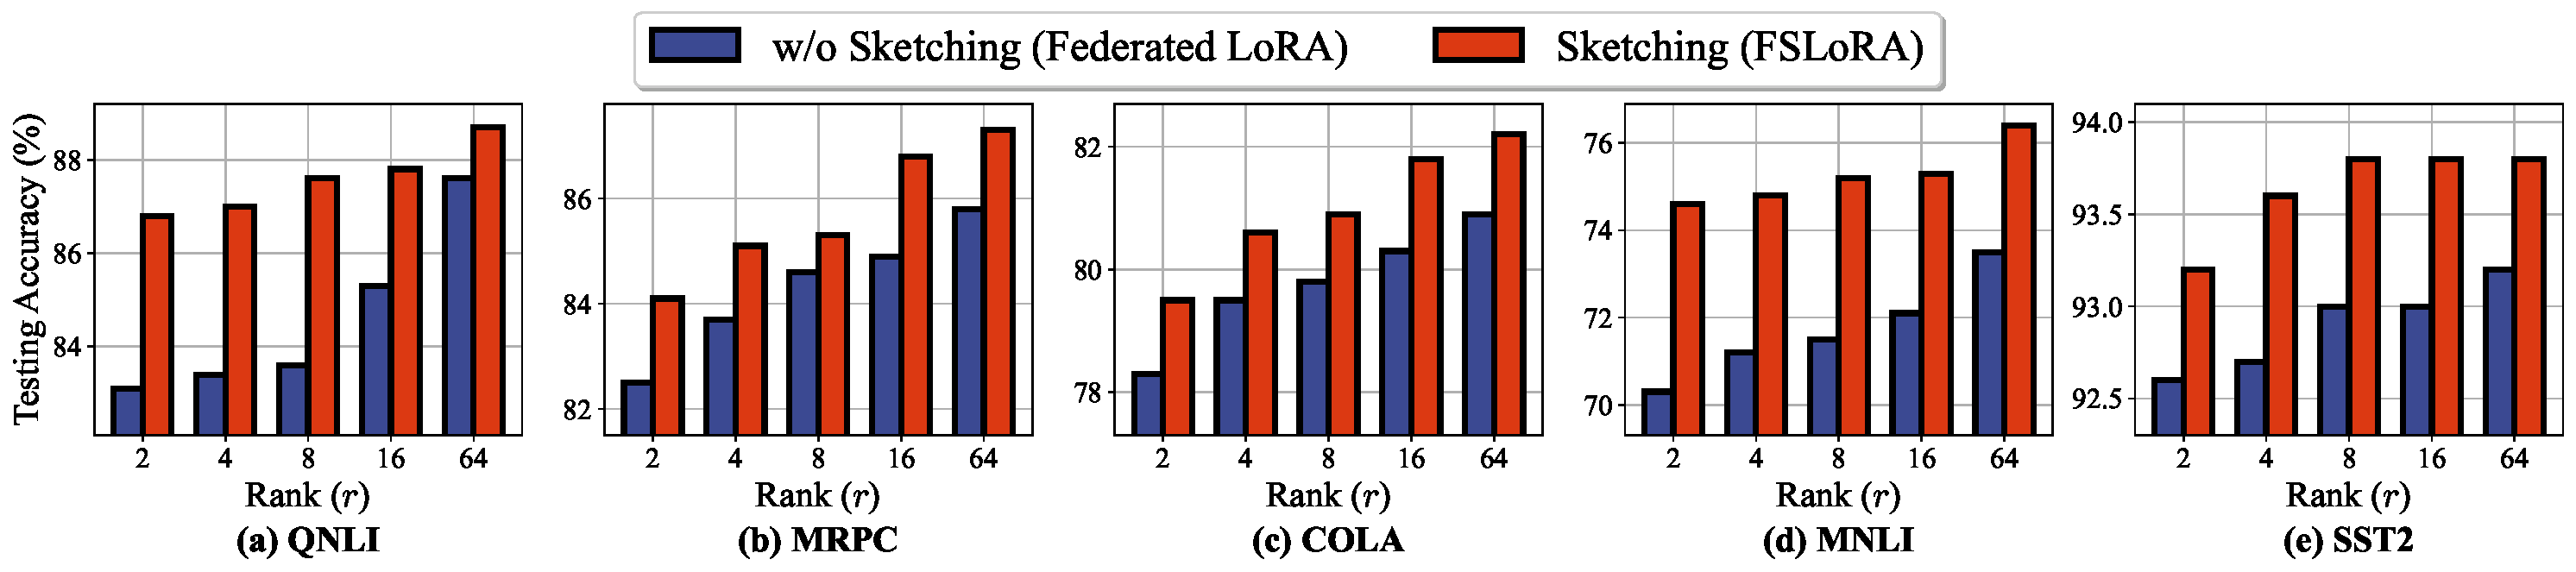
\includegraphics[width=\linewidth]{Figure/Results_RoBERTa_detail.pdf}
    \vspace{-5mm}
    \caption{Comparison between FSLoRA with and without sketching (the latter equivalent to Federated LoRA) where the upload budget for clients is set to \(100 \times\) the size of the global LoRA modules at each rank. 
    %The experiment is performed on the GLUE benchmark and the RoBERTa model. 
    FSLoRA obtains a better performance, validating its communication efficiency.
    }
    \vspace{-4mm}
    \label{fig:Results_GLUE_r}
\end{figure*}
 
\begin{figure*}[h]
    \centering
    % First subfigure
    \subfigure[Comparison of FSLoRA with and without sketching, with an upload budget \(80 \times\) the size of the global LoRA modules at each rank.]{
        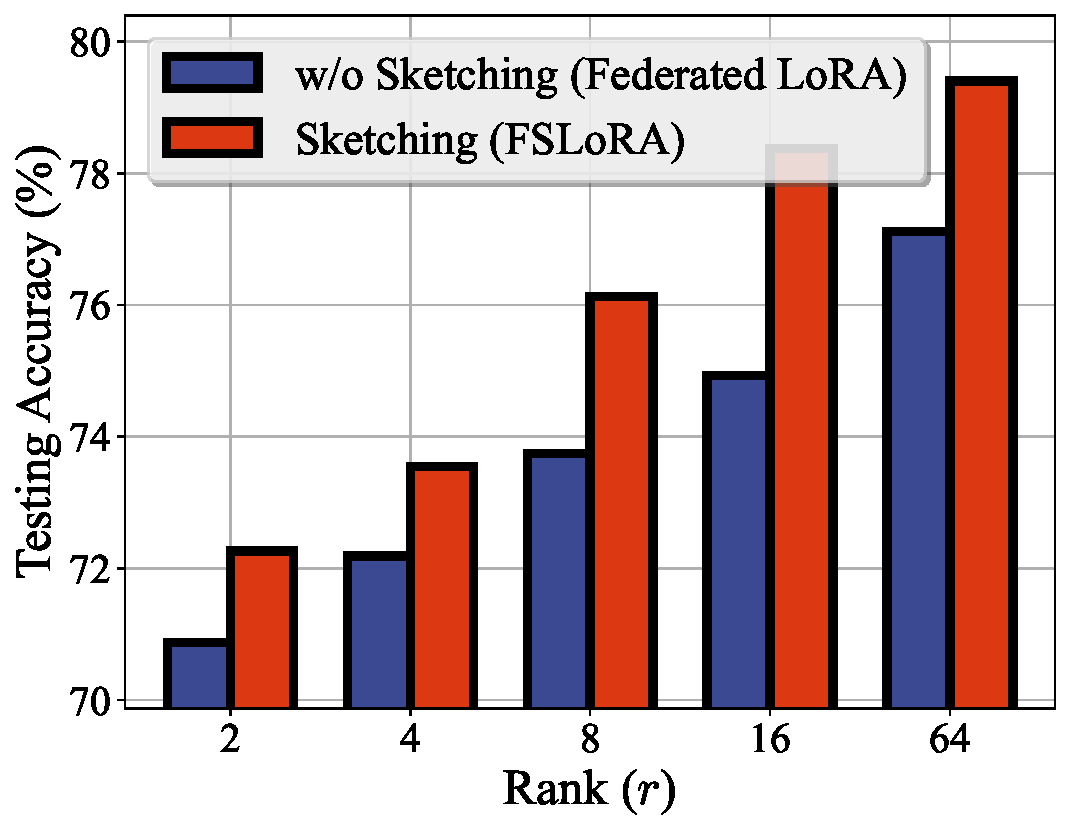
\includegraphics[width=0.3\linewidth]{Figure/Results_LLaMA.pdf} % Replace with your image
        \label{fig:rank_varying}
    }
    \hspace{1mm} % Space between subfigures
    % Second subfigure
    \subfigure[Impact of the rank of global LoRA modules on FSLoRA, given a fixed rank $k_i$ for the updated submatrices at the clients.]{
        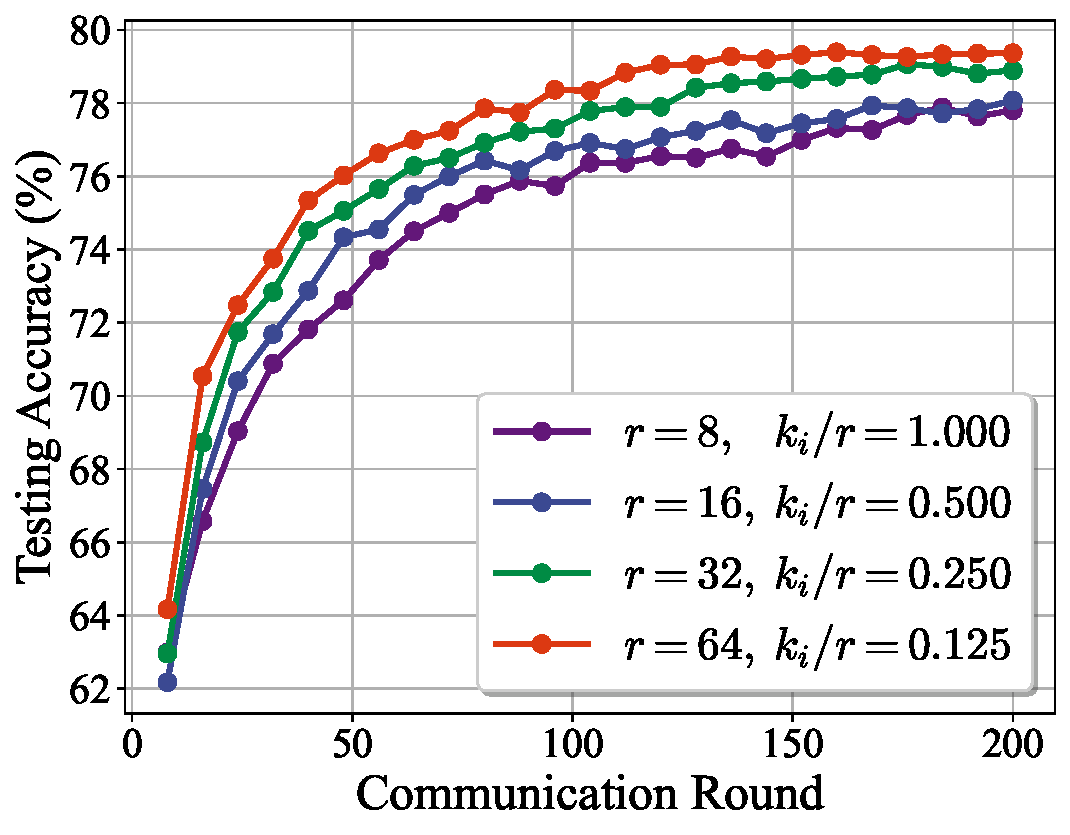
\includegraphics[width=0.3\linewidth]{Figure/Impact_global_rank.pdf} % Replace with your image
        \label{fig:global_rank}
    }
    \hspace{1mm} % Space between subfigures
    % Third subfigure
    \subfigure[Impact of the sketching ratio on FSLoRA's performance under a fixed rank $r=64$ for the global LoRA modules.]{
        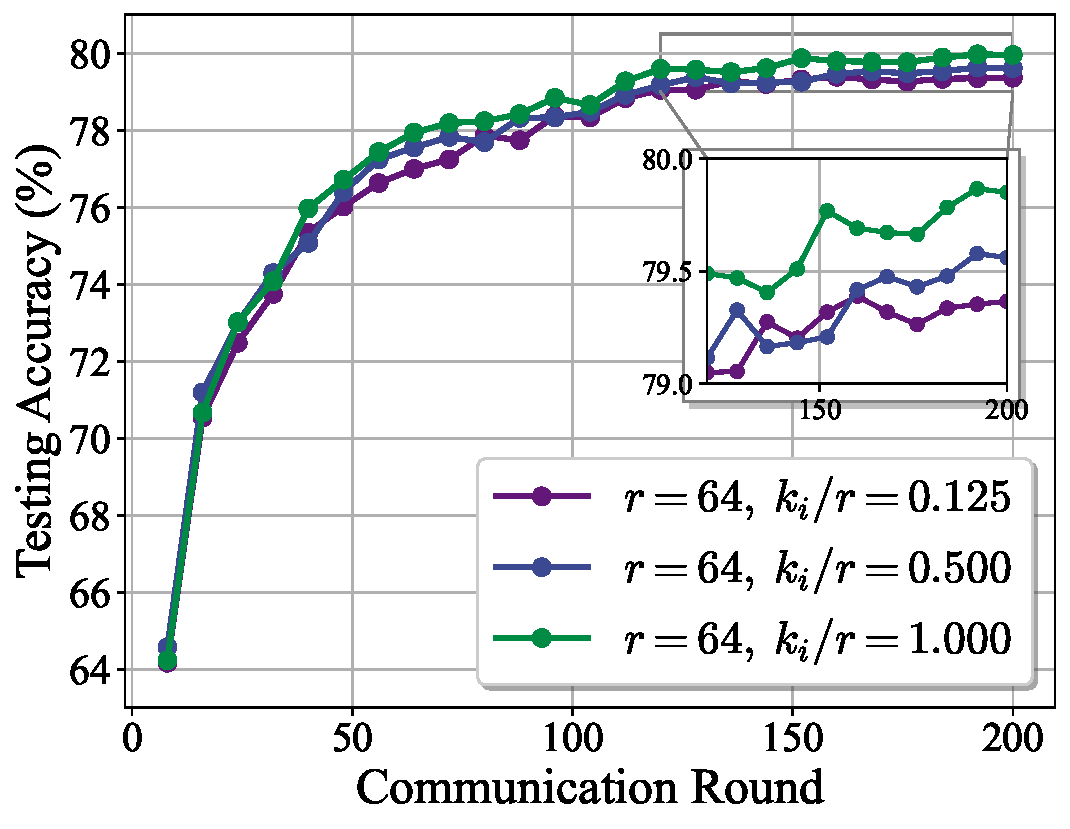
\includegraphics[width=0.3\linewidth]{Figure/Impact_sketching_ratio.pdf} % Replace with your image
        \label{fig:sketching_ratio}
    }
    \vspace{-2mm}
    \caption{Fine-tuning the LLaMA-3.2-3B model on the commonsense reasoning benchmark. The results are averaged over eight tasks, illustrating FSLoRA's ability to maintain strong performance while adapting to different rank and sketching configurations.}
    \label{fig:mainfigure}
    \vspace{-5mm}
\end{figure*}

\textbf{Impact of the global rank:} In Figure \ref{fig:global_rank}, we investigate the impact of the rank of the global LoRA modules on FSLoRA's performance. 
%We consider 4 cases: 1) \(r = 8,~ k_i/r = 1\), 2) \(r = 16,~ k_i/r  = 0.5\), 3) \(r = 32,~ k_i/r = 0.25\), 4) \(r = 64,~ k_i/r = 0.125\). The rank of submatrices updated by the clients is kept consistent (i.e., $k_i=8$) across all configurations. 
%We consider 4 cases: 1) \(r = 8,~ k_i = 8\), 2) \(r = 16,~ k_i  = 8\), 3) \(r = 32,~ k_i = 8\)  4) \(r = 64,~ k_i = 8\). 
We vary the rank of the global LoRA modules while keeping the rank of submatrices updated by the clients to be consistent (i.e., $k_i=8$).
This ensures that the communication and computational resources on the client side remain unchanged.
As illustrated in Figure \ref{fig:global_rank}, FSLoRA maintains stable convergence across all the configurations. Moreover, FSLoRA demonstrates improved performance as the global rank increases.
This observation confirms that the proposed sketching mechanism enables resource-constrained systems to reap the benefits of a higher global rank, striking an effective balance between efficiency and performance.
%This observation validates that using a large rank for the global LoRA modules results in a more expressive model. Moreover, the proposed sketching mechanism enables resource-constrained systems to effectively benefit from a large rank.
%Furthermore, the proposed sketching mechanism enables resource-constrained systems to reap the benefits of a higher global rank, striking an effective balance between efficiency and performance.


\textbf{Impact of sketching ratio:} Finally, we investigate the impact of the sketching ratio on FSLoRA's performance by maintaining a constant global LoRA rank $r=64$ while varying the sketching ratio \(k_i/r\) in the range \(\{0.125, 0.5, 1\}\). 
As shown in Figure \ref{fig:sketching_ratio}, there is a slight performance degradation as the sketching ratio decreases, which is consistent with our theoretical analysis. This reflects an inherent tradeoff: while a larger sketching ratio improves convergence and accuracy, a smaller ratio reduces both computational and communication overhead. Notably, the observed degradation remains minor, highlighting FSLoRA's ability to maintain strong performance even under constrained resources. This demonstrates its effectiveness in balancing efficiency and accuracy, making it well-suited for resource-limited scenarios.

%From Figure \ref{fig:sketching_ratio}, we see that there is a slight performance degradation as the sketching ratio decreases, which aligns with our theoretical analysis. This observation reflects the inherent tradeoff: while a larger sketching ratio enables a better convergence result, a smaller sketching ratio reduces both computational and communication overhead. Notably, the slight performance degradation observed demonstrates FSLoRA's ability to effectively balance efficiency and accuracy, underscoring its advantage in scenarios with limited resources.

\textbf{Further experiments:} 
Results with more clients under broader heterogeneity, as well as with a larger model, are reported in Appendix \ref{appen:broader_heterogeneity} and Appendix \ref{appen:larger_model}, respectively. Appendix \ref{appen:further_experiments} provides detailed per-task comparisons on the commonsense reasoning benchmark corresponding to Figures \ref{fig:rank_varying} and \ref{fig:global_rank}. The impact of varying the number of local updates $H$ is studied in Appendix \ref{appen:local_updates}, while the extension to dynamic sketching ratios is presented in Appendix \ref{appen:dynamic_sketching_ratio}. Finally, Appendix \ref{appen:compression_integration} demonstrates the synergistic effect of integrating compression with sketching.


%Additional results, including detailed comparisons on each task in the commonsense reasoning benchmark corresponding to Figures \ref{fig:rank_varying} and \ref{fig:global_rank}, the integration of communication compression and sketching, and the experiments with more devices, are provided in Appendix \ref{appen:further_experiments}. 

%\textcolor{red}{We can also talk about results with more clients here once they are ready}

\section{Conclusion}\label{sec:conclusion}
%We have proposed FSLoRA, a novel on-device collaborative LLM fine-tuning framework. Under the assistance of the sketching mechanism, FSLoRA could maintain high-rank LoRA modules on the server to enhance performance while enabling devices to flexibly update only a subset of parameters through sketching matrices, thus balancing efficiency and effectiveness in heterogeneous federated environments. We present a rigorous theoretical analysis that establishes the convergence behavior of FSLoRA and reveals how the heterogeneous ranks of updated submatrices across edge devices influence the convergence rate. Furthermore, extensive experiments across multiple datasets and models confirm the effectiveness of FSLoRA under and showcase its superior performance compared to baseline methods. A limitation of our work is that we only examine FSLoRA in the context of LLM fine-tuning, leaving its performance on pretraining unexplored and pointing to an interesting direction for future investigation.

We have proposed FSLoRA, a novel collaborative LLM fine-tuning framework that introduces a sketching mechanism to enhance both performance and efficiency in resource-constrained systems. By maintaining large-rank LoRA modules on the server and allowing clients to selectively update submatrices based on the sketching ratios, FSLoRA effectively adapts to heterogeneous communication and computational constraints. We provide a rigorous convergence analysis of FSLoRA that characterizes how the sketching ratios affect the convergence rate. Finally, we confirmed the effectiveness of FSLoRA through extensive experiments across multiple datasets and models.
%Furthermore, we characterize how the sketching ratios influence the convergence rate. Finally, we confirm the effectiveness of FSLoRA through extensive experiments across multiple datasets and models. 
%A limitation of our work is that we only examine FSLoRA in the context of LLM fine-tuning, leaving its performance on pretraining unexplored and pointing to an interesting direction for future investigation.
%A direction for future work is to extend FSLoRA beyond LLM fine-tuning and explore its performance in pretraining, which remains an open area for further investigation.
%A limitation of this work is the absence of a real-world deployment study that evaluates FSLoRA and baseline methods on the actual server and clients due to hardware constraints.


%\section*{Impact Statement}
%This paper makes important contributions to on-device LLM fine-tuning by developing a resource-adaptive algorithm for collaborative fine-tuning in resource-constrained systems. The focus of this work is on the technical advancement of LLM fine-tuning algorithms. While this research has potential societal impacts, it primarily addresses technical challenges and does not necessitate a specific discussion on societal consequences.
%This paper presents work whose goal is to advance the field of Machine Learning. There are many potential societal consequences of our work. By reducing computational and communication overheads in resource-constrained, heterogeneous environments, our approach facilitates on-device federated fine-tuning of LLMs, thereby broadening access to advanced language technologies in areas such as mobile devices.

\begin{comment}
\clearpage

\textbf{Impact of Rank:} Fixing sketching ratio, varying the rank.  In Table \ref{tab:rank_varying}, we compare the performance of the proposed FSLoRA and the vanilla Federated LoRA under the homogeneous rank scenario. The rank varies in range \(\{2, 4, 8, 16, 32, 64\}\). The sketching ratio is fixed as $k/r = 0.5$ for our approach. 
As we can see from Table \ref{tab:rank_varying}, both methods enjoy better performance as increasing rank, which can be attributed to the fact that a large rank brings a more accurate approximation to the full rank model and the use of rank-stabilized technique \citep{kalajdzievski2023rankstabilizationscalingfactor}. 
At the same rank, our approach demonstrates performance comparable to the baseline, highlighting its effectiveness. While there is a slight performance drop in most of the tasks considered, this is due to the sketching method updating only a subset of the parameters in the LoRA modules, which introduces a minor trade-off for the communication and computation benefits offered by our approach.



In Figure \ref{}, we compare the communication cost required by the proposed FSLoRA and the federated LoRA for achieving a preset testing accuracy. Specifically, the testing accuracy thresholds are set to $\%$, $\%$, $\%$, $\%$, and $\%$ for QNLI, MRPC, CoLA, MNLI, SST-2, and QQP, respectively. For this comparison, the rank is fixed at $r=64$, and the sketching ratio is set to $k/r = 0.5$. As shown in Figure \ref{}, our approach significantly reduces communication costs compared to the baseline, demonstrating the efficiency and effectiveness of the proposed Sketching LoRA.




\begin{table*}[t]
%\vspace{-4mm}
\caption{
The performance comparison between the proposed FSLoRA with a homogeneous sketching ratio $0.5$ and the vanilla Federated LoRA on the GLUE benchmark based on the RoBERTa model across different ranks. 
}
%\vspace{-.5mm}
\centering
\resizebox{\textwidth}{!}{

\begin{tabular}{@{}lcccccccccccccccc@{}}
\toprule

\multirow{2.6}{*}{Rank} & \multicolumn{2}{c}{QNLI} & \multicolumn{2}{c}{MRPC} & \multicolumn{2}{c}{CoLA} & \multicolumn{2}{c}{MNLI} & \multicolumn{2}{c}{SST-2} & \multicolumn{2}{c}{QQP}  & \multicolumn{2}{c}{AVG} \\
\cmidrule(lr){2-3} \cmidrule(lr){4-5} \cmidrule(lr){6-7} \cmidrule(lr){8-9} \cmidrule(lr){10-11} \cmidrule(lr){12-13} \cmidrule(lr){14-15}

~ & \scriptsize FSLoRA & \scriptsize FedLoRA & \scriptsize FSLoRA & \scriptsize FedLoRA & \scriptsize FSLoRA & \scriptsize FedLoRA & \scriptsize FSLoRA & \scriptsize FedLoRA & \scriptsize FSLoRA & \scriptsize FedLoRA & \scriptsize FSLoRA & \scriptsize FedLoRA & \scriptsize FSLoRA & \scriptsize FedLoRA \\
\midrule

r = 2 & 86.8 & 86.5 & 84.1 & 84.4 & 79.5 & 79.5 & 74.6 & 74.7 & 93.2 & 93.2 & 0 & 85.3 & 0 & 0 \\
r = 4 & 87.0 & 86.8 & 85.1 & 85.3 & 80.6 & 80.6 & 74.8 & 74.4 & 93.6 & 93.6 & 0 & 85.3 & 0 & 0 \\
r = 8 & 87.6 & 87.8 & 85.3 & 85.6 & 80.9 & 81.5 & 75.2 & 75.2 & 93.8 & 93.8 & 0 & 85.1 & 0 & 0 \\
r = 16 & 87.8 & 88.1 & 86.8 & 86.1 & 81.8 & 81.2 & 75.3 & 75.7 & 93.8 & 93.8 & 0 & 85.4 & 0 & 0 \\
r = 32 & 88.0 & 88.5 & 87.3 & 85.6 & 82.2 & 81.9 & 75.7 & 76.0 & 93.5 & 93.4 & 0 & 85.1 & 0 & 0 \\
r = 64 & 88.7 & 89.2 & 87.3 & 87.5 & 82.2 & 82.3 & 76.4 & 76.2 & 93.8 & 94.0 & 0 & 85.3 & 0 & 0 \\

\bottomrule
\end{tabular}
\label{tab:rank_varying}
}
%\vspace{-8mm}
\end{table*}

\begin{table}[h]
%\vspace{-4mm}
\caption{
\small The performance (testing accuracy) of FedLoRA on GLUE tasks based on RoBert model
}
%\vspace{-.5mm}
\centering
\resizebox{.5\textwidth}{!}{
\small
\begin{tabular}{lcccccccc}
\toprule
\small Rank & qnli & mrpc & cola & mnli & sst2 & qqp  & avg \\
\midrule
  r = 2 & 86.5 & 84.4 & 79.5 & 74.7 & 93.2 & 85.3 & 0  \\
 r = 4  & 86.8 & 85.3 & 80.6 & 74.4  & 93.6 & 85.3 & 0   \\
 r = 8  & 87.8 & 85.6 & 81.5 & 75.2 & 93.8 & 85.1 & 0  \\
r = 16  & 88.1 & 86.1 & 81.2 & 75.7 & 93.8 & 85.4 & 0  \\
r = 32 & 88.5 & 85.6 & 81.9 & 76.0 & 93.4 & 85.1 & 0  \\
r = 64 & \textbf{89.2} & \textbf{87.5} & \textbf{82.3} & \textbf{76.2} & \textbf{94.0} & 85.3 & 0  \\
\bottomrule
\end{tabular}
}
\label{tab_cifar}
%\vspace{-8mm}
\end{table}

\begin{table}[h]
%\vspace{-4mm}
\caption{
\small The performance (testing accuracy) of Sketching LoRA on GLUE tasks based on RoBert model. Sketching ratio $0.5$
}
%\vspace{-.5mm}
\centering
\resizebox{.5\textwidth}{!}{
\small
\begin{tabular}{lcccccccc}
\toprule
\small Rank & qnli & mrpc & cola & mnli & sst2 & qqp  & avg \\
\midrule
  r = 2 & 86.8 & 84.1 & 79.5 & 74.6 & 93.2 & 0 & 0  \\
 r = 4  & 87.0 & 85.1 & 80.6 & 74.8  & 93.6 & 0 & 0   \\
 r = 8  & 87.6 & 85.3 & 80.9 & 75.2 & 93.8 & 0 & 0  \\
r = 16  & 87.8 & 86.8 & 81.8 & 75.3 & 93.8 & 0 & 0  \\
r = 32 & 88.0 & 87.3 & 82.2 & 75.7 & 93.5 & 0 & 0  \\
r = 64 & \textbf{88.7} & \textbf{87.3} & \textbf{82.2} & \textbf{76.4} & \textbf{93.8} & 0 & 0  \\
\bottomrule
\end{tabular}
}
\label{tab_cifar}
%\vspace{-8mm}
\end{table}

\begin{table}[h]
%\vspace{-4mm}
\caption{
\small The performance (testing accuracy) of FedLoRA on GLUE tasks based on RoBert model (Under the same communication cost as the corresponding rank of Fed-Sketching LoRA)
}
%\vspace{-.5mm}
\centering
\resizebox{.5\textwidth}{!}{
\small
\begin{tabular}{lcccccccc}
\toprule
\small Rank & qnli & mrpc & cola & mnli & sst2 & qqp  & avg \\
\midrule
  r = 2 & 83.1 & 82.5 & 78.3 & 70.3 & 92.6 & 83.0 & 0  \\
 r = 4  & 83.4 & 83.7 & 79.5 & 71.2  & 92.7 & 83.3 & 0   \\
 r = 8  & 83.6 & 84.6 & 79.8 & 71.5 & 93.0 & 83.1 & 0  \\
r = 16  & 85.3 & 84.9 & 80.3 & 72.1 & 93.0 & 83.5 & 0  \\
r = 32 & 86.2 & 85.3 & 80.7 & 73.1 & 93.2 & 84.0 & 0  \\
r = 64 & \textbf{87.6} & \textbf{85.8} & \textbf{80.9} & \textbf{73.5} & \textbf{93.2} & \textbf{84.7} & 0  \\
\bottomrule
\end{tabular}
}
 
\vspace{-8mm}
\end{table}

\begin{table}[t]
%\vspace{-4mm}
\caption{
\small The performance (testing accuracy) of Sketching LoRA (heterogeneous) on GLUE tasks based on the RoBert model. Rank $r=64$. %Sketching ratio $\{0,25,0.5,0.75\}$
}
%\vspace{-.5mm}
\centering
\resizebox{.5\textwidth}{!}{
\small
\begin{tabular}{lcccccccc}
\toprule
\small Sketching ratio  & qnli & mrpc & cola & mnli & sst2 & qqp  & avg \\
\midrule
$\{0.25,0.5,0.75\}$ & \textbf{88.0} & \textbf{87.3} & \textbf{82.2} & \textbf{76.4} & \textbf{93.5} & \textbf{85.8} & 0  \\
$\{0.125, 0.25,0.5,0.75\}$ & \textbf{88.0} & \textbf{87.3} & \textbf{82.2} & \textbf{76.4} & \textbf{93.5} & \textbf{85.8} & 0  \\
\bottomrule
\end{tabular}
}
\label{tab_cifar}
%\vspace{-8mm}
\end{table}

\clearpage
\end{comment}

\begin{comment}
\section*{Impact Statement}
This paper makes important contributions to on-device LLM fine-tuning by developing a resource-adaptive algorithm for collaborative fine-tuning in resource-constrained systems. The focus of this work is on the technical advancement of LLM fine-tuning algorithms. While this research has potential societal impacts, it primarily addresses technical challenges and does not necessitate a specific discussion on societal consequences.
%This paper presents work whose goal is to advance the field of Machine Learning. There are many potential societal consequences of our work. By reducing computational and communication overheads in resource-constrained, heterogeneous environments, our approach facilitates on-device federated fine-tuning of LLMs, thereby broadening access to advanced language technologies in areas such as mobile devices.
\end{comment}

\bibliography{ref.bib}
\bibliographystyle{abbrvnat}
%\bibliographystyle{splncs04}




\begin{comment}
\section{Formulation}
\begin{equation}\label{lora_formulation}
    \min_{\bf{B} {\bf S}, \bf{A}} f(\bf B,{\bf A}) \eqdef \mathbb{E}_{\xi \sim \mathcal{D}} \left[ \ell ({\bf W_0 + \bf B{\bf A}}, \xi)\right]
\end{equation}
where $f$
%\mathbb{R}^{m \times r} \times \mathbb{R}^{r \times n} \rightarrow \mathbb{R}
denotes the empirical loss, \({\bf W}_{0}\) denotes the pretrained model, ${\bf B} \in \mathbb{R}^{m\times r},  {\bf A}\in \mathbb{R}^{r\times n}$ are LoRA modules, \(\ell\) is the sample-wise loss function, and \(\mathcal{D}\) is the dataset used for fine-tuning.

\begin{equation}\label{fed_lora_formulation}
\begin{aligned}
    \min_{\bf{B}, \bf{A}} f(\bf B,{\bf A}) &\eqdef \frac{1}{N} \sum_{i=1}^{N} f_i(\bf B,{\bf A}) \\
    f(\bf B,{\bf A}) &\eqdef  \mathbb{E}_{\xi \sim \mathcal{D}_i} \left[ \ell ({\bf W}_{0} + {\bf B} {\bf A}, \xi)\right],
\end{aligned}
\end{equation}
where $f_i: \mathbb{R}^{m \times n} \rightarrow \mathbb{R}$ denotes the empirical loss at client \(i\), \(N\) denotes the number of clients, and the frozen model \({\bf W}_{0}\) are shared by all the clients.


\begin{equation}\label{lora_formulation_ours}
\begin{aligned}
\min_{\bf B,{\bf A}} f^{\mathcal{S}}(\bf B,{\bf A}) &\eqdef  \frac{1}{N} \sum_{i=1}^N f_i^{\mathcal{S}} (\bf B,{\bf A})\\
f_i^{\mathcal{S}}(\bf B,{\bf A}) &\eqdef  \mathbb{E}_{ \sim \mathcal{S}_i; \xi \sim \mathcal{D}_i} \left[ \ell ({\bf W}_{0} + {\bf B}\bf S{\bf A}, \xi)\right],
\end{aligned}
\end{equation}
where ${\bf W}_{0}$ denotes the pretrained model, ${\bf B} \in \mathbb{R}^{m\times r},  {\bf A}\in \mathbb{R}^{r\times n}$ are LoRA modules, \(\ell\) is the sample-wise loss function, \(\mathcal{D}_i\) is the local dataset of client \(i\), and \(\mathcal{S}_i\) represents the sketching matrix set for client $i$.
\end{comment}

\newpage
\appendix


\begin{center}
    {\bf\Large Appendix}
\end{center}

\startcontents[sections]
\printcontents[sections]{l}{1}{\setcounter{tocdepth}{3}}


\newpage


\section{Comparison of Computation, Memory, and Communication}\label{appen:com_memo_comparison}
\textbf{Computation and memory:}
Let $P$ and $q$ denote the memory cost of the full model and the global LoRA module (rank $r$), respectively. The computational cost is expressed with the big O notation. Forward and backward computations, as well as activation memory, are omitted as they are identical across all the considered methods. The results are summarized in Tables  \ref{tab:com_memo_comparison_client} and \ref{tab:com_memo_comparison_server}, where $m$ and $n$ denote the shape of the base model, $k_i$ denotes the LoRA rank for client $i$, $H$ denotes the number of iterations per round, and $N$ is the number of clients. Additionally, the results for the vanilla Federated LoRA, denoted as FedLoRA, are reported under the case of homogeneous LoRA ranks, i,e., $k_i = r$. 

\begin{table}[H]
\caption{
Client-side computation load and memory usage comparison.
}
\label{tab:com_memo_comparison_client}
\centering
%\begin{adjustbox}{width=\textwidth}
\begin{tabular}{@{}lcc@{}}
\toprule
{Method} & {Memory} & {Computation (per round)} \\
\midrule
FedLoRA &
$P + q$ &
$\mathcal{O}(Hr(m + n))$ \\
HeteroLoRA &
$P + \frac{k_i}{r}q$ &
$\mathcal{O}(Hk_i(m + n))$ \\
FlexLoRA &
$P + \frac{k_i}{r}q$ &
$\mathcal{O}(Hk_i(m + n))$ \\
{FLoRA} &
$P + \max\left\{\sum_{i=1}^N \frac{k_i}{r}q, P\right\}$ &
$\mathcal{O}\left(Hk_i(m + n)) + (\sum_{i=1}^N k_i)mn + mn \right)$ \\
FSLoRA &
$P \!+\! \frac{k_i}{r}q$ &
$\mathcal{O}(Hk_i(m + n))$ \\
\bottomrule
\end{tabular}
%\end{adjustbox}
\end{table}

\begin{table}[H]
\caption{
Server-side computation load and memory usage comparison.
}
\label{tab:com_memo_comparison_server}
\centering
%\begin{adjustbox}{width=\textwidth}
\begin{tabular}{@{}lcc@{}}
\toprule
{Method} & {Memory} & {Computation (per round)} \\
\midrule
FedLoRA &
$N q$ &
$\mathcal{O}(N(m + n) r)$ \\
{HeteroLoRA} &
$\sum_{i=1}^N \frac{k_i}{r}q$ &
$\mathcal{O}(N(m + n)r)$ \\
{FlexLoRA} &
$\max\left\{\sum_{i=1}^N \frac{k_i}{r}q, 2P\right\}$ &
$\mathcal{O}\left((\sum_{i=1}^N k_i)mn + Nmn + \min\{m,n\}mn \right)$ \\
{FLoRA} &
$\sum_{i=1}^N \frac{k_i}{r}q$ &
$\mathcal{O}\left((\sum_{i=1}^N k_i)(m + n)\right)$ \\
 {FSLoRA} &
$\sum_{i=1}^N \frac{k_i}{r}q$ &
$\mathcal{O}(N(m + n)r)$ \\
\bottomrule
\end{tabular}
%\end{adjustbox}
\vspace{-3mm}
\end{table}

As shown in Tables  \ref{tab:com_memo_comparison_client} and \ref{tab:com_memo_comparison_server}, FSLoRA matches HetLoRA in both computation and memory cost. FLoRA introduces additional client-side overhead due to merging LoRA modules. FlexLoRA incurs extra server-side costs from conducting SVD on the full model. In summary, FSLoRA guarantees convergence with minimum overhead.

\textbf{Communication:}
We detailed the communication load for baselines and our methods in Table \ref{tab:communication_comp}, where $q$ denotes the communication cost of a global LoRA module with rank $r$, $k_i$ denotes the local LoRA rank for client $i$, $m$ and $n$ denote the shape of the base model, and $N$ denotes the number of clients.

\begin{table}[h]
\centering
\caption{Communication complexity, assuming float 32 parameters and binary sketching indices.}
\begin{tabular}{lccccc}
\toprule
& {FedLoRA} & {HeteroLoRA} & {FlexLoRA} & {FLoRA} & {FSLoRA} \\
\midrule
{Uplink} & $q$ & $\frac{k_i}{r}q$ & $\frac{k_i}{r}q$ & $\frac{k_i}{r}q$ & $\frac{k_i}{r}q$ \\
{Downlink} & $q$ & $q$ & $q$ & $\sum_{i=1}^{N} \frac{k_i}{r}q $ & $q(1+\frac{Nr}{32mn})$ \\
\bottomrule
\end{tabular}
\label{tab:communication_comp}
\vspace{-2mm}
\end{table}
%For uplink, the communication overhead for transmitting updated local LoRA modules are the same for these four algorithms. For downlink, FLoRA needs to broadcast stacked LoRA modules, HeteroLoRA and FlexLoRA need to broadcast the updated global LoRA modules, and FSLoRA needs to broadcast the global LoRA modules and sketching matrix. Note that the extra communication load introduced by transmitting the sketching matrix is negligible compared to global LoRA modules, as it involves only \emph{binary sketching indices} (i.e., the diagonal elements of the sketching matrix). For example, considering the LLaMA-3.2-3B model, under the LoRA setup in our experiment, the global LoRA modules have $66060288$ parameters. This translates to $252$ MB for broadcasting (in float32). When the rank is set to $r=64$ for the global LoRA modules, the sketching indices require only $64$ bits per client (applies to all LoRA layers). Even with 100 clients, sketching indices add just $0.78$ KB ($0.0003\%$ over $252$ MB).

For the uplink, all four heterogeneous LoRA algorithms incur the same communication overhead for transmitting updated local LoRA modules, which is lower than that of FedLoRA.
For the downlink, FLoRA requires broadcasting the stacked LoRA modules, while HeteroLoRA and FlexLoRA broadcast the updated global LoRA modules. FSLoRA, on the other hand, broadcasts both the global LoRA modules and additional sketching matrices.
The extra communication introduced by the sketching matrices is negligible compared to that of the global LoRA modules, as it consists only of \emph{binary sketching indices} (i.e., the diagonal elements of the sketching matrix). For instance, in the case of the LLaMA-3.2-3B model under our experimental LoRA configuration, the global LoRA modules contain 66,060,288 parameters, equivalent to approximately 252 MB when using float32. With a global rank of $r = 64$, the sketching indices require only 64 bits per client, covering all LoRA layers. Even with 100 clients, the total sketching overhead is merely 0.78 KB, which accounts for only 0.0003\% of the global LoRA modules.


\section{Difference between FSLoRA and FedBCGD}\label{appen:difference_to_fbcgd}


Both FSLoRA and federated block coordinate gradient descent (FedBCGD) \citep{liu2024fedbcgd} are motivated by client heterogeneity but are designed for fundamentally different deployment contexts. FedBCGD partitions the full model $\mathbf{x} = [\mathbf{x}_1, \ldots, \mathbf{x}_N, \mathbf{x}_s]$, assigning each block $\mathbf{x}_j$ to a subset of clients with similar resource constraints, while the shared block $\mathbf{x}_s$ is optimized across all clients. While this block-partitioning strategy is effective for smaller models, it relies on explicit and static allocation, which can limit scalability and flexibility. As such, FedBCGD and similar block coordinate methods based on the full model are less suitable for federated LLM fine-tuning.

FSLoRA, in contrast, builds on LoRA and introduces sparse diagonal sketching. Given a sketch matrix $\bf{S}$, the gradients of the loss $\ell({\bf W}_0 + {\bf BSA}, \xi)$ with respect to the LoRA matrices ${\bf B}$ and ${\bf A}$
are sparse: only selected columns of ${\bf B}$ and rows of ${\bf A}$ are updated in each round.
By configuring the rank and sparsity of the sketch matrix $\bf{S}$, FSLoRA flexibly controls both the computational and communication load per client, enabling adaptation to heterogeneous client capabilities.

The distinctions between FedBCGD and FSLoRA are summarized in Table \ref{conceptual_distinctions}. To wrap up, these two algorithms are tailored for distinct purposes and deployment contexts.

\begin{table}[h]
\caption{
Conceptual distinctions between FSLoRA and FedBCGD.
}
\label{conceptual_distinctions}
\centering
\begin{tabular}{@{}lllll@{}}
\toprule
{Aspect} & {FedBCGD} & {FSLoRA} \\
\midrule
Partition Type & Explicit \& static & Random \& sketching-based \\
Model Scope & Full model & LoRA modules \\
Adaptation Strategy & Assign different blocks & Adjust sketch rank (sparsity) \\
\bottomrule
\end{tabular}
\vspace{-3mm}
\end{table}

\section{Justification for Random-$k$ Sketching}\label{appen:discussion_alternative_sketching}

FSLoRA is built upon Random-$k$ diagonal sketching due to two key properties:
\begin{itemize}[leftmargin=*]
    \item \textbf{Submatrix selection.} Given a sparse diagonal matrix $\mathbf{S}_i$, we have
    \[
        \mathbf{BS}_i\mathbf{A} = \sum_{j \in \mathcal{I}_i} s_j \mathbf{b}_j \mathbf{a}_j^\top 
        = [\mathbf{b}_j]_{j \in \mathcal{I}_i} \operatorname{diag}\{s_j\}_{j \in \mathcal{I}_i} [\mathbf{a}_j^\top]_{j \in \mathcal{I}_i},
    \]
    where \(\mathcal{I}_i\) corresponds to the index set of non-zero diagonal entries of \(\mathbf{S}_i\) and $\mathbf{b}_j$ and $\mathbf{a}_j^\top$ denote the $j$-th column of module $\mathbf{B}$ and the $j$-th row of module $\mathbf{A}$, respectively.
    In other words, with Random-$k$ sketching, only a subset of $\mathbf{B}$'s columns and $\mathbf{A}$'s rows are activated for client $i$. 
    The \emph{sparse diagonal structure} effectively reduces local training cost for each client. 
    \item \textbf{Unbiasedness for convergence.} When $\mathbf{S}_i$ is a Random-$k$ diagonal matrix with $k_i$ nonzero diagonal entries $s_j = \frac{r}{k_i}$, we have 
    \[
        \mathbb{E}[\mathbf{BS}_i\mathbf{A}] = \mathbf{BA}.
    \]
    This unbiasedness is critical for our convergence analysis.
\end{itemize}

\begin{table}[h]
\centering
\caption{Accuracy comparison of Random-$k$ sketching and importance-based sketching under the commonsense reasoning benchmark with the LLaMA-3.2-3B model. Random-$k$ sketching achieves better performance.}
\small
\resizebox{\linewidth}{!}{
\begin{tabular}{lccccccccc}
\toprule
\textbf{Importance metric} & ARC-c & ARC-e & BoolQ & HSwag & OBQA & PIQA & SIQA & Wino & Avg. \\
\midrule
$\|a\| \|b\|$           & 71.9 & 86.5 & 55.2 & 75.4 & 73.4 & 81.1 & 72.5 & 69.7 & 73.2 \\
$\|a\| + \|b\|$         & 72.1 & 86.4 & 64.5 & 76.8 & 70.8 & 82.2 & 71.3 & 69.3 & 74.2 \\
\rowcolor{ours} Random-$k$              & 75.8 & 86.7 & 69.7 & 81.4 & 80.4 & 83.9 & 76.2 & 78.8 & 79.1 \\
\bottomrule
\end{tabular}
}
\label{tab:alternative_sketching}
\end{table}

In addition, we experimentally compare Random-$k$ sketching with importance-based sketching. For importance-based sketching, we sample (sketch) $k_i$ components from $\{ \mathbf{b}_j \mathbf{a}_j^\top \}_{j=1}^r$ with probability set as the importance scores, e.g., $\|\mathbf{b}_j\|_2 + \|\mathbf{a}_j\|_2$ or spectral norm $\|\mathbf{b}_j\|_2 \cdot \|\mathbf{a}_j\|_2$. The results are shown in Table \ref{tab:alternative_sketching}. The results show that Random-$k$ diagonal sketching outperforms these choices for importance-based sketching. This may be because these importance measures are heuristic and do not reliably reflect actual contribution. Moreover, such sketching violates the unbiasedness property, complicating theoretical guarantees. While improved importance-based methods may enhance performance and remain a promising direction for future investigation, our current empirical and theoretical results favor random sketching.


\section{Compatibility of FSLoRA with Secure Aggregation}\label{appen:secure_aggregation}
The aggregation of FSLoRA is compatible with secure aggregation. Taking the aggregation of module $\mathbf{B}$ as an example, we illustrate this below. 

In FSLoRA, client updates are sparse matrices with non-zero values only in columns indexed by $\mathcal{I}_i \subset [r]$, size $|\mathcal{I}_i| = k_i$. With secure aggregation, each client apply \emph{additive masking}:
\[
\tilde{\mathbf{B}}_i = \Delta \mathbf{B}_i + \mathbf{R}_i,
\]
where mask $\mathbf{R}_i$ satisfies $\operatorname{supp}(\mathbf{R}_i) \subseteq (u,v): u \in [m], v \in \mathcal{I}_i$ and $\sum_{i=1}^N \mathbf{R}_i = 0$. That is, the mask has non-zero entries only in the client's active columns, and all masks together sum to zero to preserve correctness. Such masks can be constructed following the classical protocol: for each pair of clients $(i,j)$, define a random matrix
\[
\mathbf{M}_{ij} = - \mathbf{M}_{ji} \in \mathbb{R}^{m \times r}, 
\quad \operatorname{supp}(\mathbf{M}_{ij}) \subseteq (u,v) \;|\; u \in [m], \, v \in \mathcal{I}_i \cap \mathcal{I}_j,
\]
and then construct its total mask
\[
\mathbf{R}_i = \sum_{j>i} \mathbf{M}_{ij} - \sum_{j<i} \mathbf{M}_{ji}.
\]

During uploading, client $i$ sends the masked $k_i$ non-zero columns of $\tilde{\mathbf{B}}_i$, and then the server adds the corresponding padding and averages them as:
\[
\sum_{i=1}^N \tilde{\mathbf{B}}_i 
= \sum_{i=1}^N \left( \Delta \mathbf{B}_i + \mathbf{R}_i \right) 
= \sum_{i=1}^N \Delta \mathbf{B}_i,
\]
which matches the aggregation of module $\mathbf{B}$ in \eqref{model_aggregation}. The aggregation of module $\mathbf{B}$ in FSLoRA is thus compatible with secure aggregation. 

We can draw the same conclusion for module $\mathbf{A}$ under the same derivation.


\section{Empirical Validation of Assumptions}\label{appen:justification_assumption}

In the context of LLM fine-tuning, both the magnitude of stochastic gradients and gradients in LLM fine-tuning are in a mild range since:
\begin{itemize}[leftmargin=*]
    \item Transformer-based LLMs use \emph{LayerNorm} and \emph{scaled softmax attention}, which stabilize activations and suppress gradient spikes.
    \item Fine-tuning starts from a well-pretrained model already near a local minimum, leading to smaller gradients.
    \item The fine-tuning dataset does not typically contain strong contradictory signals to what the model already knows, resulting in a relatively flat loss surface. 
\end{itemize}

To further support this empirically, we report the statistics of the expected norm of the stochastic gradients 
$\mathbb{E}\|\nabla_{\mathbf{X}} \tilde{\ell}(\mathbf{X},\xi;\mathbf{S})\|$ 
over approximately $4500$ samples for 4 representative clients with different sketching ratios. The table below reports the minimum and maximum expected norm among 30 randomly sampled model states $\mathbf{X} = [\mathbf{B}; \mathbf{A}]$.

\begin{table}[h!]
\caption{Statistics of the expected norm of stochastic gradients across clients.\label{tab:gradient_norm}}
\centering
\small
\begin{tabular}{ccccc}
\toprule
\textbf{Client ID} & \textbf{Number of samples} & \textbf{Rank} & \textbf{Min} & \textbf{Max} \\
\midrule
1 & 4580 & 4  & 0.1286 & 0.9499 \\
2 & 4216 & 19 & 0.1284 & 0.7069 \\
3 & 4873 & 9  & 0.1237 & 0.5774 \\
4 & 5124 & 32 & 0.1499 & 0.8066 \\
\bottomrule
\end{tabular}
\end{table}


As we can see from Table \ref{tab:gradient_norm}, the expected norm, i.e., $\mathbb{E}_{\xi \sim \mathcal{D}_i, \mathbf{S}\sim \mathcal{S}_i}\|\nabla_{\mathbf{X}} \tilde{\ell}(\mathbf{X},\xi;\mathbf{S})\|$, is in a moderate range. Notably, the variance is upper-bounded by the expected squared gradient norm:
\[
\mathbb{E}_{\xi \sim \mathcal{D}_i, \mathbf{S}\sim \mathcal{S}_i} \|\nabla_{\mathbf{X}} \tilde{\ell}(\mathbf{X},\xi;\mathbf{S}) - \nabla_{\mathbf{X}} f_i^{\mathcal{S}}(\mathbf{X})\|^2 
\leq \mathbb{E}_{\xi \sim \mathcal{D}_i, \mathbf{S}\sim \mathcal{S}_i}\|\nabla_{\mathbf{X}} \tilde{\ell}(\mathbf{X},\xi;\mathbf{S})\|^2.
\]
Therefore, it is generally not hard to find a $\sigma$ and $\rho$ to make Assumption~\ref{varaince_assumption} hold.

On the other hand, we have
\begin{equation}
\begin{aligned}
& \left\| \nabla_{\bf X} f_i^{\mathcal{S}}({\bf X}) \!-\! \nabla_{\bf X} f^{\mathcal{S}}(\bf X) \right\|^2 \\
\leq &  2 \left\| \nabla_{\bf X} f_i^{\mathcal{S}}({\bf X})  \right\|^2 +   2 \left\| \nabla_{\bf X} f^{\mathcal{S}}(\bf X) \right\|^2 \\
\leq & 2 \left\| \nabla_{\bf X} f_i^{\mathcal{S}}({\bf X})  \right\|^2 +   2 \frac{1}{N}\sum_{i=1}^N \left\| \nabla_{\bf X} f_i^{\mathcal{S}}({\bf X}) \right\|^2 \\
\leq & 2 \mathbb{E}_{\xi \sim \mathcal{D}_i, \mathbf{S}\sim \mathcal{S}_i}\|\nabla_{\mathbf{X}} \tilde{\ell}(\mathbf{X},\xi;\mathbf{S})\|^2 +   2 \frac{1}{N}\sum_{i=1}^N \mathbb{E}_{\xi \sim \mathcal{D}_i, \mathbf{S}\sim \mathcal{S}_i}\|\nabla_{\mathbf{X}} \tilde{\ell}(\mathbf{X},\xi;\mathbf{S})\|^2,
\end{aligned}
\end{equation}
where the first inequality follows Cauchy-Schwarz inequality, while the last inequality follows Jensen's inequality.
Thus, the deviation can be controlled by the expected gradient norm, which we empirically found to be moderate (see Table \ref{tab:gradient_norm}). Hence, it is reasonable to impose an upper bound on $\left\| \nabla_{\bf X} f_i^{\mathcal{S}}({\bf X}) \!-\! \nabla_{\bf X} f^{\mathcal{S}}(\bf X) \right\|^2 $ as in Assumption \ref{assumption:gradient_dissimilarity}.


\section{Evaluation under Broader Heterogeneity and Increased Number of Clients}\label{appen:broader_heterogeneity}

To accommodate a larger number of clients, we extend FSLoRA (Algorithm~\ref{alo_flora}) to support \emph{partial client participation}. Specifically, at each round, the server samples a subset of clients, distributes the current global LoRA modules to them, and aggregates only the updates from these clients. Throughout this section, we fix the partial participation size to 10, i.e., 10 clients are sampled in each round.

\subsection{Increasing Resource Heterogeneity and the Number of Clients}\label{appen:more_devices_more_heterogeneity}

We extend our experiments on LLaMA-3.2-3B with the commonsense reasoning benchmark to $50$ clients. We adopt Dirichlet-based partitioning for dataset splits.
Specifically, the commonsense reasoning benchmark includes $8$ tasks, and we partitioned them based on the Dirichlet distribution to construct task heterogeneity among $50$ clients. The Dirichlet concentration parameter is set to $\alpha = 0.1$.
We simulate client resource heterogeneity via different LoRA rank distributions (beyond the limited sketching ratio considered in Section \ref{sec:experiment}). More capable clients are assigned higher ranks, reflecting varying compute capacities. We consider two different rank distributions: normal and heavy-tail distributions in the range $[4, 64]$.

\textbf{Normal distribution:} Ranks are sampled from a normal distribution with mean $\mu = \frac{a + b}{2}$ and standard deviation $\sigma = \frac{b - a}{6}$, where $a=4$ and $b=64$.
This models a balanced distribution of client capabilities centered around the middle of the range.

%\textbf{Uniform distribution:} Local ranks are uniformly sampled from the range $[4, 64]$, simulating a scenario where client capabilities are evenly distributed across a fixed range.


\textbf{Heavy-tail distribution:} We sample ranks using an inverse log-normal distribution. Specifically, we draw $x_i \sim \text{LogNormal}(\mu, \sigma)$ with $\mu = \log\left(\frac{a + b}{4}\right)$ and $\sigma = 1.0$, then set $k_i = 1/x_i$ and apply min-max normalization to scale values into the range $[a, b]$. This results in a heavy-tailed distribution where most clients receive low ranks, reflecting a scenario with many low-capability clients and a few high-capability ones.


\begin{table}[h]
\centering
\caption{Accuracy comparison under different client heterogeneity settings. FSLoRA outperforms baseline methods across both normal and heavy-tail LoRA rank distributions.}
\small
\resizebox{\linewidth}{!}{
\begin{tabular}{llccccccccc}
\toprule
{Rank setup} & Method & ARC-c & ARC-e & BoolQ & HellaSwag & OBQA & PIQA & SIQA & WinoGrande & Avg. \\
\midrule

\multirow{4}{*}{{Normal}} 
& HeteroLoRA     & 73.38 & 85.82 & 62.17 & 71.23 & 77.40 & 80.14 & 74.72 & 72.53 & 74.67 \\
& FlexLoRA       & 74.23 & 87.84 & 68.37 & 79.77 & 76.00 & 82.97 & 75.90 & 78.13 & 77.90 \\
& FLoRA   & 68.17 & 83.75 & 64.93 & 75.67 & 71.40 & 77.20 & 71.24 & 70.09 & 72.81 \\
\rowcolor{ours}& {FSLoRA}       & {75.77} & {86.95} & {69.67} & {81.53} & {80.60} & {84.06} & {76.20} & {78.85} & {79.20} \\

\midrule

\multirow{4}{*}{{Heavy-tail}} 
& HeteroLoRA     & 72.44 & 86.78 & 63.60 & 73.10 & 72.00 & 81.34 & 71.65 & 68.75 & 73.71 \\
%& FlexLoRA       & 72.95 & 86.74 & 62.13 & 75.43 & 77.40 & 80.90 & 74.72 & 72.85 & 75.39 \\
& FlexLoRA       & 73.04 & 86.70 & 62.23 & 75.57 & 78.00 & 81.12 & 74.77 & 73.32 & 75.59 \\
& FLoRA   & 67.92 & 81.90 & 64.90 & 72.77 & 74.00 & 80.41 & 75.28 & 70.24 & 73.43 \\
\rowcolor{ours}& {FSLoRA}       & {75.77} & {86.70} & {69.67} & {81.40} & {80.40} & {83.90} & {76.15} & {78.77} & {79.10} \\

\bottomrule
\end{tabular}
}
\label{tab:divice_het}
\end{table}

\begin{comment}
\begin{table*}[h]
\centering
\caption{Accuracy comparison on commonsense reasoning benchmarks under different data heterogeneity settings. FSLoRA maintains its advantage over the baselines as the data heterogeneity increases.}
\small
\resizebox{\linewidth}{!}{
\begin{tabular}{llccccccccc}
\toprule
{Data setup} & Method & ARC-c & ARC-e & BoolQ & HellaSwag & OBQA & PIQA & SIQA & WinoGrande & Avg. \\
\midrule

\multirow{4}{*}{Dir(0.5)} 
& HeteroLoRA     & 70.3 & 86.5 & 65.9 & 70.0 & 74.0 & 82.1 & 71.5 & 68.0 & 73.5 \\
& FlexLoRA       & 70.1 & 85.3 & 65.8 & 68.8 & 71.4 & 80.8 & 68.9 & 69.3 & 72.5 \\
& FLoRA   & 68.3 & 85.8 & 65.5 & 68.5 & 69.0 & 74.9 & 66.5 & 69.1 & 71.0 \\
& {FSLoRA} & {72.7} & {87.2} & {67.2} & {72.1} & {76.8} & {81.4} & {74.0} & {71.0} & {75.3} \\

\midrule

\multirow{4}{*}{Dir(0.1)} 
& HeteroLoRA     & 69.9 & 85.0 & 65.3 & 69.0 & 72.3 & 81.1 & 70.7 & 67.3 & 72.6 \\
& FlexLoRA       & 69.9 & 84.0 & 65.1 & 68.0 & 70.6 & 79.5 & 68.7 & 68.7 & 71.8 \\
& FLoRA   & 67.6 & 84.8 & 64.5 & 67.8 & 67.8 & 73.8 & 65.9 & 68.0 & 70.0 \\
& {FSLoRA} & {72.0} & {86.2} & {67.2} & {71.3} & {75.6} & {80.8} & {73.4} & {70.6} & {74.6} \\

\bottomrule
\end{tabular}
}
\label{tab:data_het}
\end{table*}
\end{comment}

As shown in Table \ref{tab:divice_het}, FSLoRA outperforms other methods under both heterogeneity settings. As we move from normal to heavy-tail, where more clients are low-resource, overall performance decreases for all methods. However, FSLoRA exhibits the smallest drop, demonstrating stronger robustness to extreme client heterogeneity.

%Figure \ref{fig:comvergence_comparison_device} compares the convergence behavior of FSLoRA and three baseline methods in different device heterogeneity scenarios. Notably, in the heavy-tail distribution case where most devices are low-resource, FSLoRA maintains stable and robust convergence while baseline methods suffer significant degradation. 


In Figure \ref{fig:comvergence_comparison_device}, we compare the convergence behavior of FSLoRA and three baseline methods under the aforementioned two types of client heterogeneity. Under the normal distribution, FlexLoRA exhibits fast initial progress but falls behind FSLoRA in final accuracy, likely due to approximation errors introduced by truncated SVD. This issue is exacerbated in the heavy-tail distribution, where low-rank clients dominate and SVD truncation causes greater distortion, further degrading FlexLoRA's performance. Similarly, HeteroLoRA's reliance on zero-padding reduces optimization efficiency, preventing it from achieving higher accuracy. 
FLoRA fails to show steady improvement as communication progresses. One potential reason is that frequent model merging and random reinitialization of LoRA modules in each round disrupt the convergence continuity. %Notably, the official implementation of FLoRA also recommends using a small number of communication rounds \cite{wang2024flora}.
%FLoRA struggles to converge in both settings. 
%one potential reason is the frequent random reinitialization of LoRA modules at each round, which disrupts convergence continuity.
In contrast, FSLoRA demonstrates robust and stable convergence across both scenarios, achieving the highest overall accuracy.


\begin{figure}[h]
    \centering
    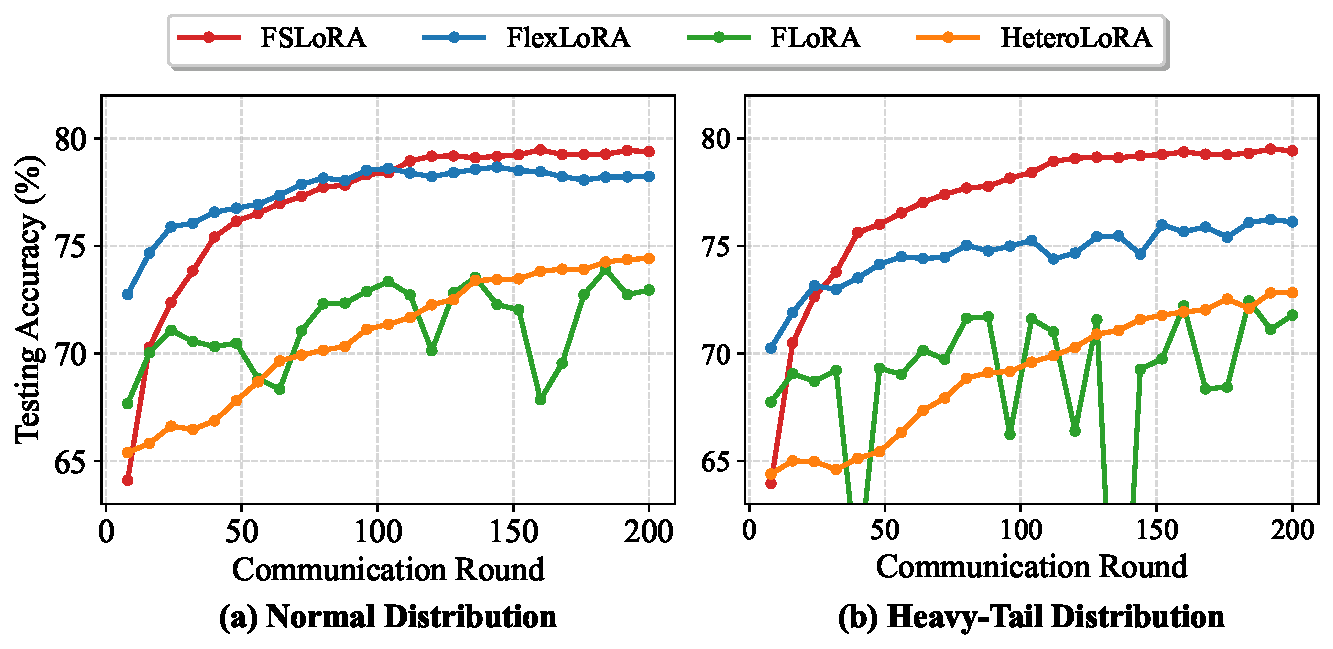
\includegraphics[width=0.8\linewidth]{Figure/convergence_comparison_device.pdf}
    %\vspace{-5mm}
    \caption{Convergence behavior of FSLoRA and baselines on the commonsense reasoning benchmark with the LLaMA-3.2-3B model. Notably, FSLoRA's per-round communication cost is at most equal to the baselines (as detailed in Appendix \ref{appen:com_memo_comparison}). Testing accuracy is averaged over eight tasks.
    }
    %\vspace{-5mm}
    \label{fig:comvergence_comparison_device}
\end{figure}

\subsection{Further Increasing the Number of Clients}
%We further evaluated the performance of FSLoRA by increasing the number of devices from $50$ to $100$. The results are presented in Table \ref{tab:more_devices}. In this setting, local ranks follow a heavy-tailed distribution as described in the previous subsection, and all other experimental configurations remain unchanged. As shown in the table, FSLoRA maintains stable performance across all benchmarks when scaling to more devices, with only a slight drop in average accuracy. This minor decline can be attributed to increased data dispersion across a larger number of devices, which potentially increases the difficulty of local training.

We further evaluated the performance of FSLoRA by increasing the number of clients to $100$. The results are presented in Table \ref{tab:more_devices}. In this setting, local ranks follow a heavy-tailed distribution as described in the previous subsection, and all other experimental configurations remain unchanged. As shown in the table, FSLoRA maintains its advantage in terms of the average performance when scaling to more clients. 


\begin{table}[h]
\centering
\caption{Accuracy comparison when the number of clients is $N=100$. FSLoRA maintains its advantage in terms of the average accuracy.}
\small
\resizebox{\linewidth}{!}{
\begin{tabular}{lccccccccc}
\toprule
Method & ARC-c & ARC-e & BoolQ & HellaSwag & OBQA & PIQA & SIQA & WinoGrande & Avg. \\
\midrule

 HeteroLoRA     & 71.76 & 86.24 & 62.57 & 68.07 & 76.60 & 79.38 & 74.10 & 69.69 & 73.55 \\
 FlexLoRA       & 73.38 & 87.54 & 69.03 & 75.27 & 78.60 & 80.47 & 74.16 & 73.80 & 76.53 \\
 FLoRA   & 69.97 & 83.25 & 67.10 & 71.67 & 73.60 & 78.94 & 72.21 & 70.80 & 73.44 \\
\rowcolor{ours} {FSLoRA}  & {74.40} & {87.54} & {70.13} & {79.90} & {79.40} & {83.57} & {76.51} & {78.93} & {78.80} \\
\bottomrule
\end{tabular}
}
\label{tab:more_devices}
\end{table}

\begin{comment}
\begin{table}[h]
\centering
\caption{
Performance of FSLoRA with different numbers of devices.}
\small
\resizebox{\linewidth}{!}{
\begin{tabular}{lccccccccc}
\toprule
Devices & ARC-c & ARC-e & BoolQ & HellaSwag & OBQA & PIQA & SIQA & WinoGrande & Avg. \\
\midrule
50  & {75.77} & {86.70} & {69.67} & {81.40} & {80.40} & {83.90} & {76.15} & {78.77} & {79.10} \\
100  & {74.40} & {87.46} & {70.13} & {79.90} & {79.40} & {83.57} & {76.51} & {78.93} & {78.79} \\
\bottomrule
\end{tabular}
}
\label{tab:more_devices}
\end{table}

\begin{table}[h]
\centering
\caption{Performance of FSLoRA with different numbers of devices.}
\small
\resizebox{\linewidth}{!}{
\begin{tabular}{llccccccccc}
\toprule
{Devices} & Method & ARC-c & ARC-e & BoolQ & HellaSwag & OBQA & PIQA & SIQA & WinoGrande & Avg. \\
\midrule

\multirow{4}{*}{$N=50$}
& HeteroLoRA     & 72.44 & 86.78 & 63.60 & 73.10 & 72.00 & 81.34 & 71.65 & 68.75 & 73.71 \\
%& FlexLoRA       & 72.95 & 86.74 & 62.13 & 75.43 & 77.40 & 80.90 & 74.72 & 72.85 & 75.39 \\
& FlexLoRA       & 73.04 & 86.70 & 62.23 & 75.57 & 78.00 & 81.12 & 74.77 & 73.32 & 75.59 \\
& FLoRA   & 67.92 & 81.90 & 64.90 & 72.77 & 74.00 & 80.41 & 75.28 & 70.24 & 73.43 \\
\rowcolor{ours}& {FSLoRA}       & {75.77} & {86.70} & {69.67} & {81.40} & {80.40} & {83.90} & {76.15} & {78.77} & {79.10} \\

\midrule

\multirow{4}{*}{$N=100$} 
& HeteroLoRA     & 71.76 & 86.24 & 62.57 & 68.07 & 76.60 & 79.38 & 74.10 & 69.69 & 73.55 \\
& FlexLoRA       & 73.38 & 87.54 & 69.03 & 75.27 & 78.60 & 80.47 & 74.16 & 73.80 & 76.53 \\
& FLoRA   & 69.97 & 83.25 & 67.10 & 71.67 & 73.60 & 78.94 & 72.21 & 70.80 & 73.44 \\
\rowcolor{ours}& {FSLoRA}  & {74.40} & {87.46} & {70.13} & {79.90} & {79.40} & {83.57} & {76.51} & {78.93} & {78.79} \\
\bottomrule
\end{tabular}
}
\label{tab:more_devices}
\end{table}
\end{comment}



\subsection{Varying the Level of Data Heterogeneity}

In Table \ref{tab:data_het}, we investigate the impact of the degree of data heterogeneity on performance. We increase the heterogeneity by decreasing the Dirichlet concentration parameter from $\alpha = 1$ to $\alpha = 0.1$. 
The local ranks follow the heavy-tail distribution described in the previous subsection, and all other experimental configurations remain consistent with Appendix \ref{appen:more_devices_more_heterogeneity}. 
As observed from Table \ref{tab:data_het}, the performance of all methods degrades as heterogeneity increases. FSLoRA consistently achieves higher accuracy.

\begin{table}[h]
\centering
\caption{Accuracy comparison under different data heterogeneity settings. FSLoRA maintains its advantage over the baselines as the data heterogeneity increases. The number of clients is set to $50$.}
\small
\resizebox{\linewidth}{!}{
\begin{tabular}{llccccccccc}
\toprule
{Data setup} & Method & ARC-c & ARC-e & BoolQ & HellaSwag & OBQA & PIQA & SIQA & WinoGrande & Avg. \\
\midrule

\multirow{4}{*}{Dir(1)} 
& HeteroLoRA     & 72.18 & 86.11 & 62.57 & 73.10 & 77.60 & 79.82 & 74.26 & 69.46 & 74.39 \\
& FlexLoRA       & 74.06 & 87.25 & 65.67 & 74.90 & 78.80 & 81.01 & 74.16 & 74.27 & 76.27 \\
& FLoRA   & 70.14 & 83.29 & 67.27 & 71.60 & 73.60 & 78.73 & 72.16 & 70.96 & 73.47 \\
\rowcolor{ours}& {FSLoRA}       & {75.85} & {87.50} & {70.93} & {81.47} & {81.00} & {82.86} & {76.66} & {78.53} & {79.35} \\

\midrule

\multirow{4}{*}{Dir(0.1)} 
& HeteroLoRA     & 72.44 & 86.78 & 63.60 & 73.10 & 72.00 & 81.34 & 71.65 & 68.75 & 73.71 \\
%& FlexLoRA       & 72.95 & 86.74 & 62.13 & 75.43 & 77.40 & 80.90 & 74.72 & 72.85 & 75.39 \\
& FlexLoRA       & 73.04 & 86.70 & 62.23 & 75.57 & 78.00 & 81.12 & 74.77 & 73.32 & 75.59 \\
& FLoRA   & 67.92 & 81.90 & 64.90 & 72.77 & 74.00 & 80.41 & 75.28 & 70.24 & 73.43 \\
\rowcolor{ours}& {FSLoRA}       & {75.77} & {86.70} & {69.67} & {81.40} & {80.40} & {83.90} & {76.15} & {78.77} & {79.10} \\

\bottomrule
\end{tabular}
}
\label{tab:data_het}
\end{table}

% \begin{figure}[h]
%     \centering
%     \includegraphics[width=0.8\linewidth]{Figure/convergence_comparison_data.pdf}
%     %\vspace{-5mm}
%     \caption{Convergence behavior of FSLoRA and baselines on the commonsense reasoning benchmark with the LLaMA-3.2-3B model. Testing accuracy is averaged over eight tasks.
%     }
%     %\vspace{-5mm}
%     \label{fig:comvergence_comparison_data}
% \end{figure}


% In addition, Figure \ref{fig:comvergence_comparison_data} presents the convergence behavior of FSLoRA and baseline methods under varying degrees of data heterogeneity. 

\section{Experiments on LLaMA-7B}\label{appen:larger_model}

Although our primary focus is on models suitable for client-side deployment, such as RoBERTa and LLaMA-3.2-3B models, we also include experiments on the larger LLaMA-7B model to demonstrate the scalability of FSLoRA in more complex models. Specifically, we fine-tune the LLaMA-7B model on the Wizard, Dolly-15k, and Alpaca datasets and evaluate it on $1444$ MMLU samples (available at: https://github.com/ATP-1010/FederatedLLM). For Wizard and Dolly-15k, we adopt the same heterogeneous data partitioning as \citep{wang2024flora}. Since the Alpaca dataset lacks a clear task or domain structure, we apply a uniform random partitioning strategy to distribute the data across clients. We tune the \text{q\_proj} and \text{v\_proj} modules and set the local LoRA ranks $k_i\!=\![64, 32, 16, 16, 8, 8, 4, 4, 4, 4]$ for $10$ clients. The parameter settings are aligned with those in \citep{wang2024flora}. 
%Table \ref{tab:llama7b_results} reports the results, with FSLoRA numbers sourced directly from \citep{wang2024flora}.

\begin{table}[h]
\centering
\caption{Performance comparison on LLaMA-7B model.}
\begin{tabular}{lcccc}
\toprule
{Method} & {Wizard} & {Dolly-15k} & {Alpaca} & {Avg} \\
\midrule
HeteroLoRA         & 27.15           & 26.70              & 28.74           & 27.53        \\
FlexLoRA         & 28.25           & 35.60             & 30.40           & 31.42        \\
FLoRA    & 27.91           & 28.50              & 29.54           & 28.65        \\
\rowcolor{ours} FSLoRA & 30.33  & 40.79     & 30.68  & 33.93 \\
\bottomrule
\end{tabular}
\label{tab:llama7b_results}
\end{table}


As shown in Table \ref{tab:llama7b_results}, FSLoRA achieves the highest average performance across all three datasets compared to baselines. These results demonstrate FSLoRA's potential for effective fine-tuning with the large-scale LLaMA-7B model under heterogeneous client settings.


% {\color{red}
% \section{Experiments on more models and datasets}
% }
%\newpage 
\section{Further Experiments}

In this section, we provide additional results, including detailed per-task comparisons from the commonsense reasoning benchmark corresponding to Figures \ref{fig:rank_varying} and \ref{fig:global_rank}. In addition, we further investigate the impact of the number of local updates $H$ on the convergence, the robustness of FSLoRA under dynamic sketching ratio, and the integration of communication compression and sketching.

%compare the communication costs required to achieve a preset testing accuracy

\subsection{Further Details on the Ablation Study}\label{appen:further_experiments}

\textbf{Impact of sketching:} In Figure \ref{fig:llama_detail_fix_budget}, we compare the performance of FSLoRA with and without sketching on eight tasks from the commonsense reasoning benchmark using the LLaMA-3.2-3B model. Notably, FSLoRA without sketching is equivalent to the vanilla Federated LoRA. For FSLoRA with sketching, we apply a uniform sketching ratio of \(k_i/r = 0.5\) across all distributed clients. 
The uploading budget for each client is set to \(200\) times the size of the full global LoRA modules at the corresponding rank. It is clear that FSLoRA with sketching consistently outperforms its non-sketched counterpart across these eight tasks, demonstrating the effectiveness of sketching in improving performance.


\begin{figure}[h!]
    \centering
    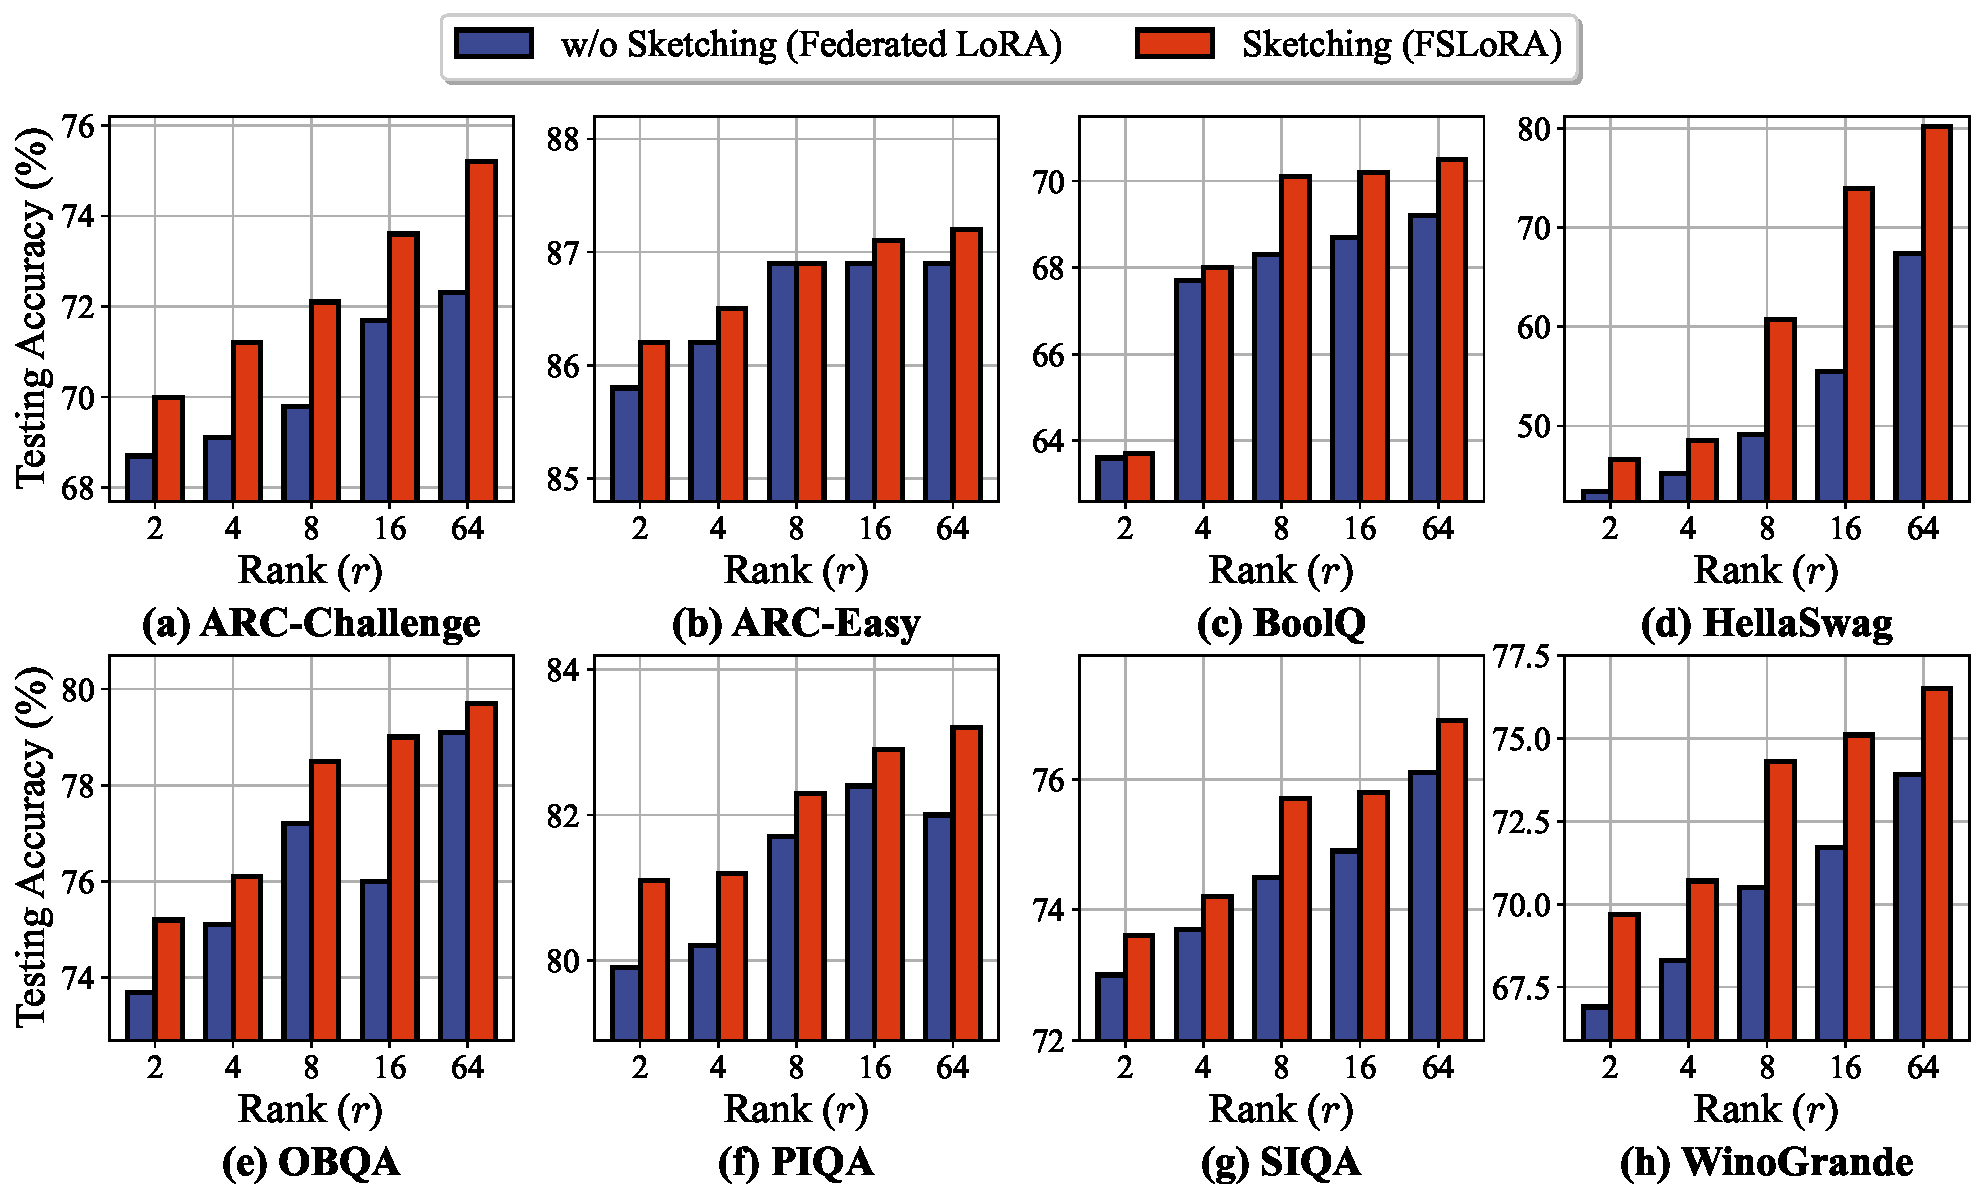
\includegraphics[width=\linewidth]{Figure/Results_LLaMA_detail.pdf}
    \caption{Comparison of FSLoRA with and without sketching, with an upload budget \(200 \times\) the global LoRA module size at each rank. This is based on the commonsense reasoning benchmark and the LLaMA-3.2-3B model. We observe that the sketching mechanism improves performance across all considered tasks. The average accuracy of the eight tasks is shown in Figure \ref{fig:rank_varying}.}
    \label{fig:llama_detail_fix_budget}
\end{figure}

\begin{figure}[h!]
    \vspace{-2mm}
    \centering
    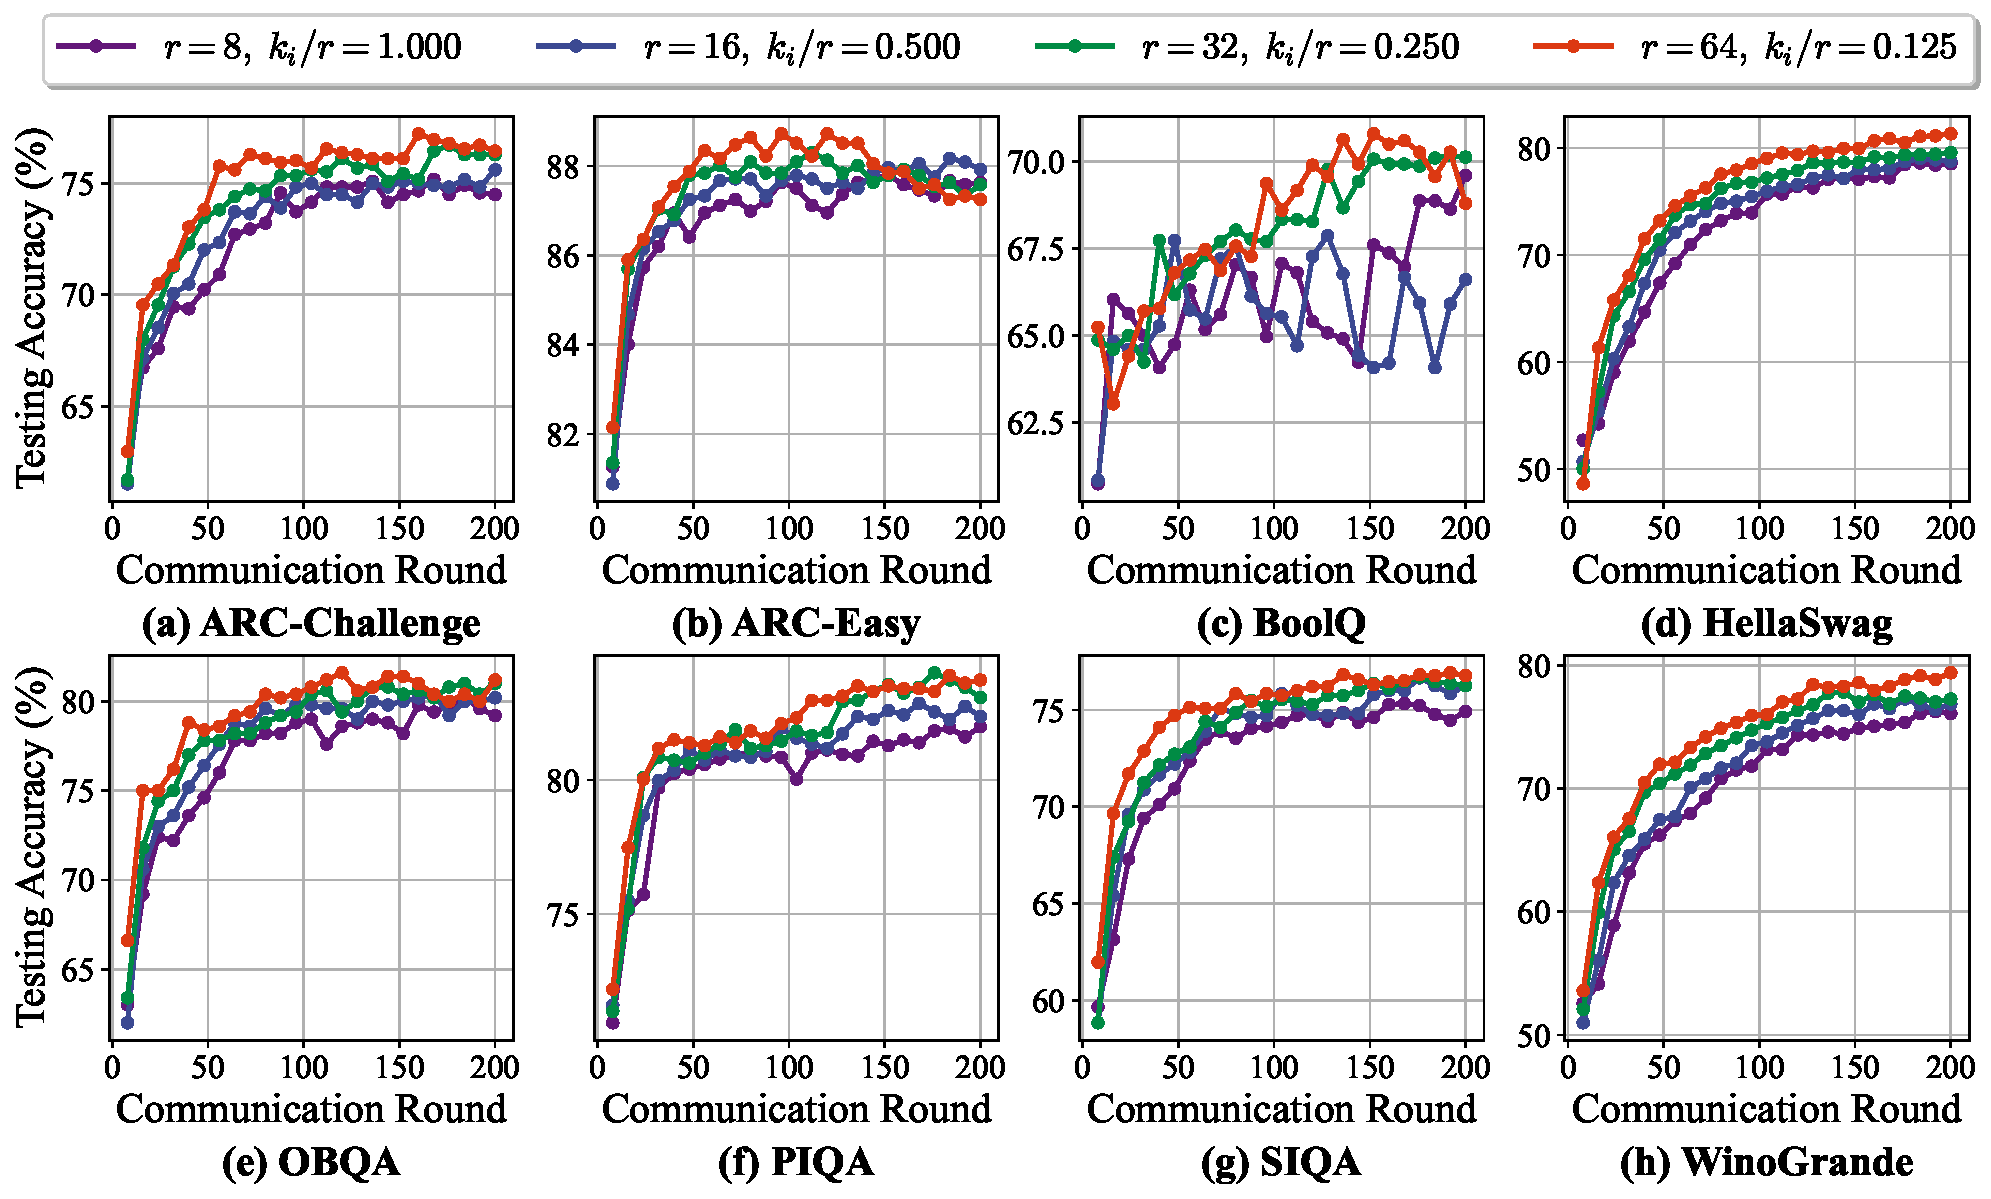
\includegraphics[width=\linewidth]{Figure/Impact_global_rank_detail}
    \caption{Impact of the rank of global LoRA modules on FSLoRA, given a fixed rank for the updated submatrices at the clients. This is based on the commonsense reasoning benchmark and the LLaMA-3.2-3B model. Overall, FSLoRA demonstrates improved performance as the global rank increases. The average accuracy of the eight tasks is shown in Figure \ref{fig:global_rank}.
    }
    \label{fig:llama_detail_global_rank}
    %\vspace{-4mm}
\end{figure}

\textbf{Impact of the global rank:} In Figure \ref{fig:llama_detail_global_rank}, we present the impact of the rank of the global LoRA modules on FSLoRA's performance across eight tasks from the commonsense reasoning benchmark. We consider four configurations: 1) \(r = 8,~ k_i/r = 1\), 2) \(r = 16,~ k_i/r = 0.5\), 3) \(r = 32,~ k_i/r = 0.25\), and 4) \(r = 64,~ k_i/r = 0.125\). The rank of submatrices updated by the clients at each iteration remains consistent across all configurations (i.e., \(k_i = 8\)), ensuring that the communication and computational resources on the client side are kept fixed for all cases. In the ARC-Easy task, performance decreases as the rank increases to $64$, potentially due to overfitting. 
%We see that the third subfigure exhibits oscillations as the sketching ratio increases. One potential explanation for this behavior is that the BoolQ task may be more sensitive to variations in the sketching ratio. 
In general, FSLoRA shows improved performance as the rank increases. 

%As shown in Figure \ref{fig:llama_detail_global_rank}, FSLoRA demonstrates improved performance overall as the global rank increases, highlighting that a larger rank for the global LoRA modules leads to a more expressive model. Furthermore, the proposed sketching mechanism enables resource-constrained systems to effectively leverage the benefits of a large global rank. We also see that the third subfigure (\textbf{BoolQ}) exhibits significant oscillations as the sketching ratio increases. One potential explanation for this behavior is that the \textbf{BoolQ} task may be more sensitive to variations in the sketching ratio, potentially due to its specific data distribution or the nature of the task requiring a more stable representation. This suggests that sensitivity to the sketching ratio may vary across tasks and should be taken into account when designing global rank configurations for different tasks.
\subsection{Impact of Local Updates}\label{appen:local_updates}
Based on the commonsense reasoning benchmark and the LLaMA-3.2-3B model, we evaluated the convergence behavior of FSLoRA under varying numbers of local updates (i.e., $H$). The experimental results are presented in Figure~\ref{fig:impact_H}. In the low-to-moderate regime of local updates (i.e., $H \in {10, 20, 100}$), FSLoRA demonstrates a clear acceleration in convergence as $H$ increases. For example, moving from $H=10$ to $H=20$ substantially reduces the number of communication rounds required to reach the same level of testing accuracy, while further increasing $H$ to $100$ yields even faster progress toward convergence. This observation indicates that a moderate increase in local updates allows clients to improve communication efficiency. However, when the number of local updates is pushed beyond this range (e.g., $H=200$), no additional convergence gain is observed. These findings align well with our theoretical analysis in Section \ref{sec:analysis}, which shows that FSLoRA can achieve a convergence speedup under certain conditions on $H$. 

\begin{figure}[h!]
    \centering
    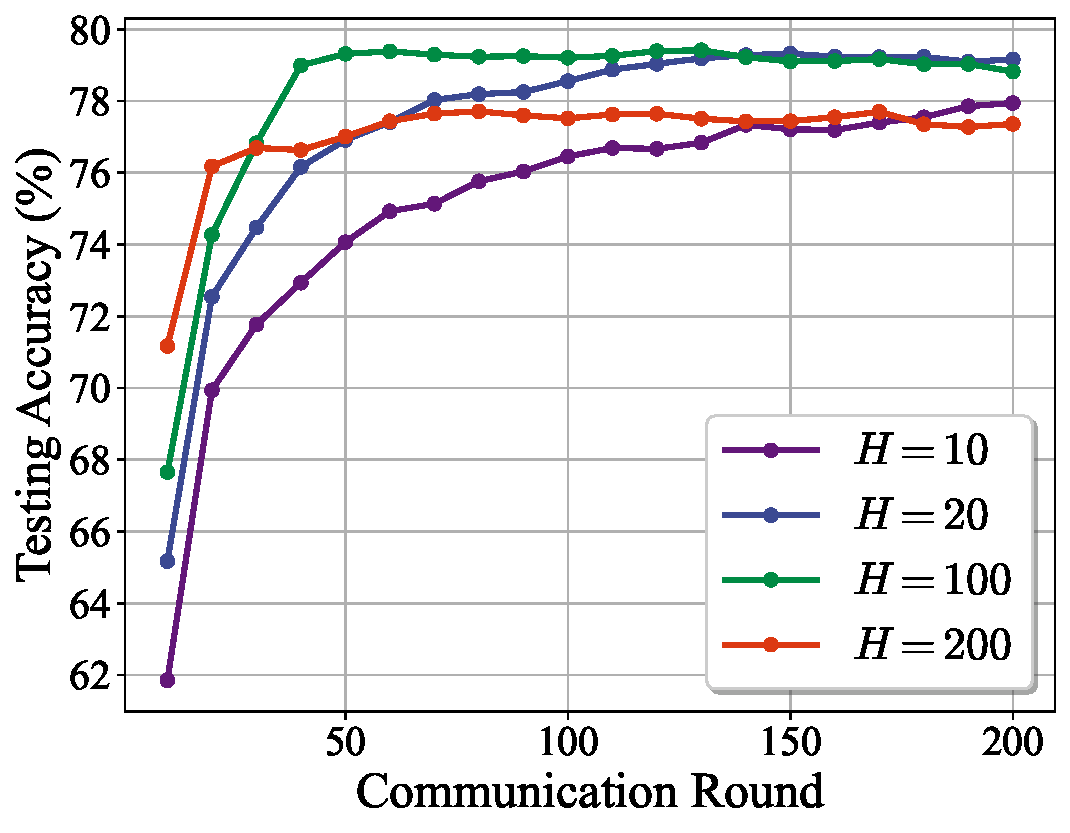
\includegraphics[width=0.4\linewidth]{Figure/Impact_H.pdf}
    \caption{Impact of the number of local updates on FSLoRA's convergence. This is based on the commonsense reasoning benchmark and the LLaMA-3.2-3B model. In a certain range, i.e., from 10 to 100, FSLoRA achieves a fast convergence as $H$ increases.
    }
\label{fig:impact_H}
\end{figure}

\subsection{Dynamic Sketching Ratios}\label{appen:dynamic_sketching_ratio}
While our primary focus is on developing a heterogeneous federated LoRA method under a standard static setup, following prior works \citep{wang2024flora,cho2024heterogeneouslorafederatedfinetuning,bai2024federatedfinetuninglargelanguage}, the proposed FSLoRA algorithm can be naturally extended to dynamic, time-varying resource environments. The modification is straightforward: we allow the sparsity levels, corresponding to the sketching ratios of FSLoRA, of the matrices in the sketching set $\mathcal{S}_i$ in Algorithm~\ref{alo_flora} to become time-varying, while keeping the remaining steps unchanged. 

We empirically validate the effectiveness of FLoRA under this dynamic setting. In the simulation, we group clients into three capability levels \emph{low}, \emph{medium}, and \emph{high}, assigned sketching ratio ranges $[0.125, 0.25]$, $[0.25, 0.5]$, and $[0.5, 1.0]$, respectively, to balance local training latencies across groups. Within each range, the sketching ratios are allowed to vary dynamically. The results, reported in Table~\ref{tab:dynamic_ratios}, show that FSLoRA maintains comparable performance when moving from the static to the dynamic case, demonstrating its robustness under time-varying sketching ratios.

\begin{table}[h]
\centering
\caption{The performance of FSLoRA under static and dynamic sketching ratios. This is based on the commonsense reasoning benchmark and the LLaMA-3.2-3B model. FSLoRA maintains comparable performance when moving from the static to the dynamic case.}
\label{tab:dynamic_ratios}
\begin{tabular}{lccccccccc}
\toprule
Ratios & ARC-c & ARC-e & BoolQ & HSwag & OBQA & PIQA & SIQA & Wino & Avg. \\
\midrule
Static  & 76.1 & 87.1 & 70.0 & 81.7 & 81.4 & 82.6 & 76.4 & 78.9 & 79.3 \\
\rowcolor{ours} Dynamic & 75.5 & 87.7 & 69.2 & 81.3 & 81.2 & 82.2 & 76.0 & 78.8 & 79.0 \\
\bottomrule
\end{tabular}
\end{table}

\subsection{Integration of Sketching and Top-k Compression}\label{appen:compression_integration} 

\begin{figure}[h]
    \centering
    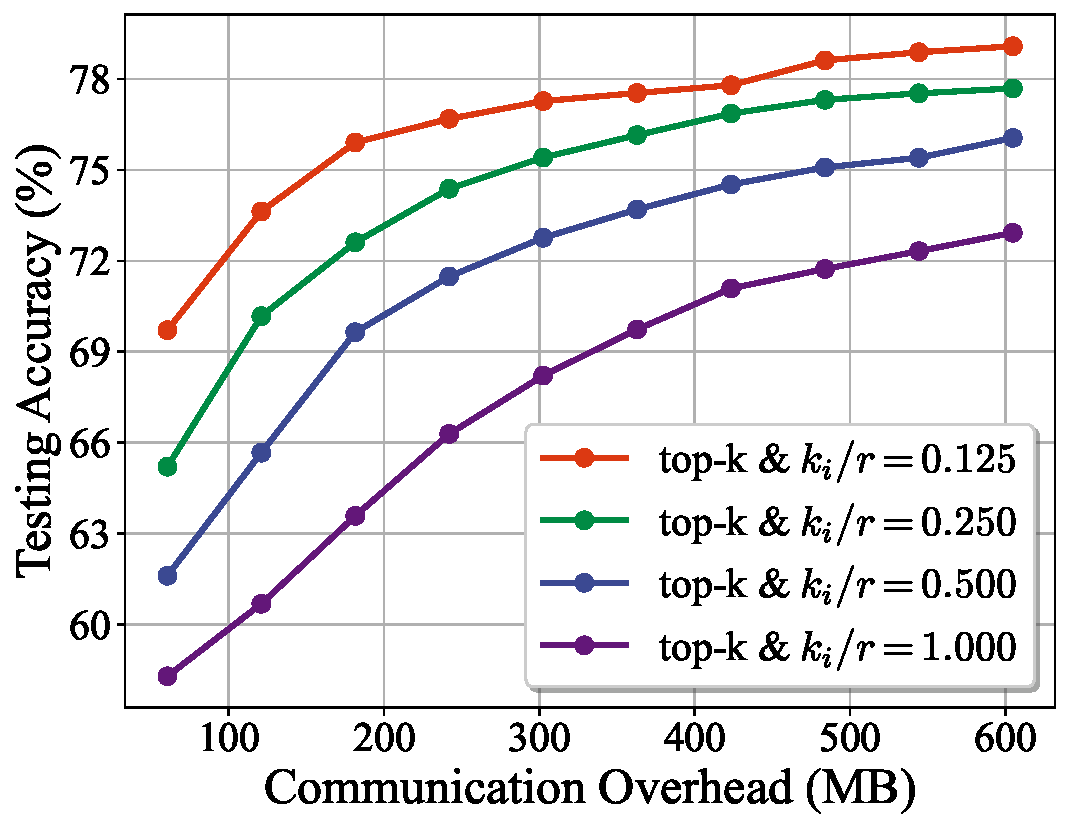
\includegraphics[width=0.4\linewidth]{Figure/Impact_topk.pdf}
    \caption{Testing accuracy versus communication overhead using float 32 precision. Lower sketching ratios achieve higher accuracy at the same communication cost, demonstrating that combining sketching with top-$k$ compression leads to more communication-efficient training.
    }
\label{fig:integration_compression_sketching}
\end{figure}

Building on the commonsense reasoning benchmark and the LLaMA-3.2-3B model, we further explore the integration of two orthogonal techniques, sketching and top-k compression, to further reduce the uplink communication overhead of clients in FSLoRA. 

Specifically, with sketching, each client activates and updates submatrices of the global LoRA weights, 
$[\mathbf{b}_j]_{j \in \mathcal{I}_i}, [\mathbf{a}_j^\top]_{j \in \mathcal{I}_i}$, which are selected at the beginning of each round:
\[
\mathbf{BS}_i\mathbf{A} = \sum_{j \in \mathcal{I}_i} \frac{r}{k_i} \mathbf{b}_j \mathbf{a}_j^\top 
= \frac{r}{k_i} [\mathbf{b}_j]_{j \in \mathcal{I}_i} [\mathbf{a}_j^\top]_{j \in \mathcal{I}_i},
\]
where $\mathbf{b}_j$ and $\mathbf{a}_j^\top$ denote the $j$-th column of module $\mathbf{B}$ and the $j$-th row of module $\mathbf{A}$, respectively. By limiting updates to submatrices $[\mathbf{b}_j]_{j \in \mathcal{I}_i}$ and $[\mathbf{a}_j^\top]_{j \in \mathcal{I}_i}$, 
FSLoRA reduces communication and computation. To further reduce communication cost, we can apply Top-$k$ compression to the uploading stage. For instance, instead of sending the full 
$\Delta [\mathbf{b}_j]_{j \in \mathcal{I}_i}$, each client transmits the compressed update 
$\operatorname{Top}_k(\Delta [\mathbf{b}_j]_{j \in \mathcal{I}_i})$.  
Sketching selects the update submatrix at the beginning of each round, 
while compression further reduces its transmission cost at the uploading stage. 
These two techniques operate at different stages and can jointly improve 
communication efficiency.

In our setup, the compression ratio is fixed at \(0.5\) for all methods, while the sketching ratio \(k_i/r\) varies over \(\{0.125, 0.25, 0.5, 1\}\). Notably, FSLoRA with sketching ratio \(k_i/r = 1\) corresponds to the vanilla Federated LoRA (i.e., without sketching).
Figure \ref{fig:integration_compression_sketching} plots testing accuracy versus communication overhead, where the x-axis represents the amount of data uploaded per client (in MB), assuming parameters are stored in float 32 precision. 
The results clearly show that integrating sketching with top-k compression further improves communication efficiency: methods with lower sketching ratios consistently achieve higher accuracy under the same communication budget, highlighting the potential of FSLoRA for scalable and communication-efficient collaborative LLM fine-tuning.

\begin{comment}
\subsection{Experiments with More Devices}
Finally, we increase the number of devices to \(50\) and repeat the comparison of FSLoRA with and without sketching. Figure \ref{fig:more_device} shows the detailed per-task comparison while Figure \ref{fig:more_device_average} shows the averaged performance comparison across these eight tasks from the commonsense reasoning benchmark. We vary the rank of the global LoRA modules in the rage \(\{4,16,64\}\). The sketching ratio is set to \(0.5\) for FSLoRA. This experiment is also based on the LLaMA-3.2-3B model. As shown in Figures \ref{fig:more_device} and \ref{fig:more_device_average}, the advantages of FSLoRA are preserved as the number of devices increases.

\begin{figure}[h!]
    \centering
    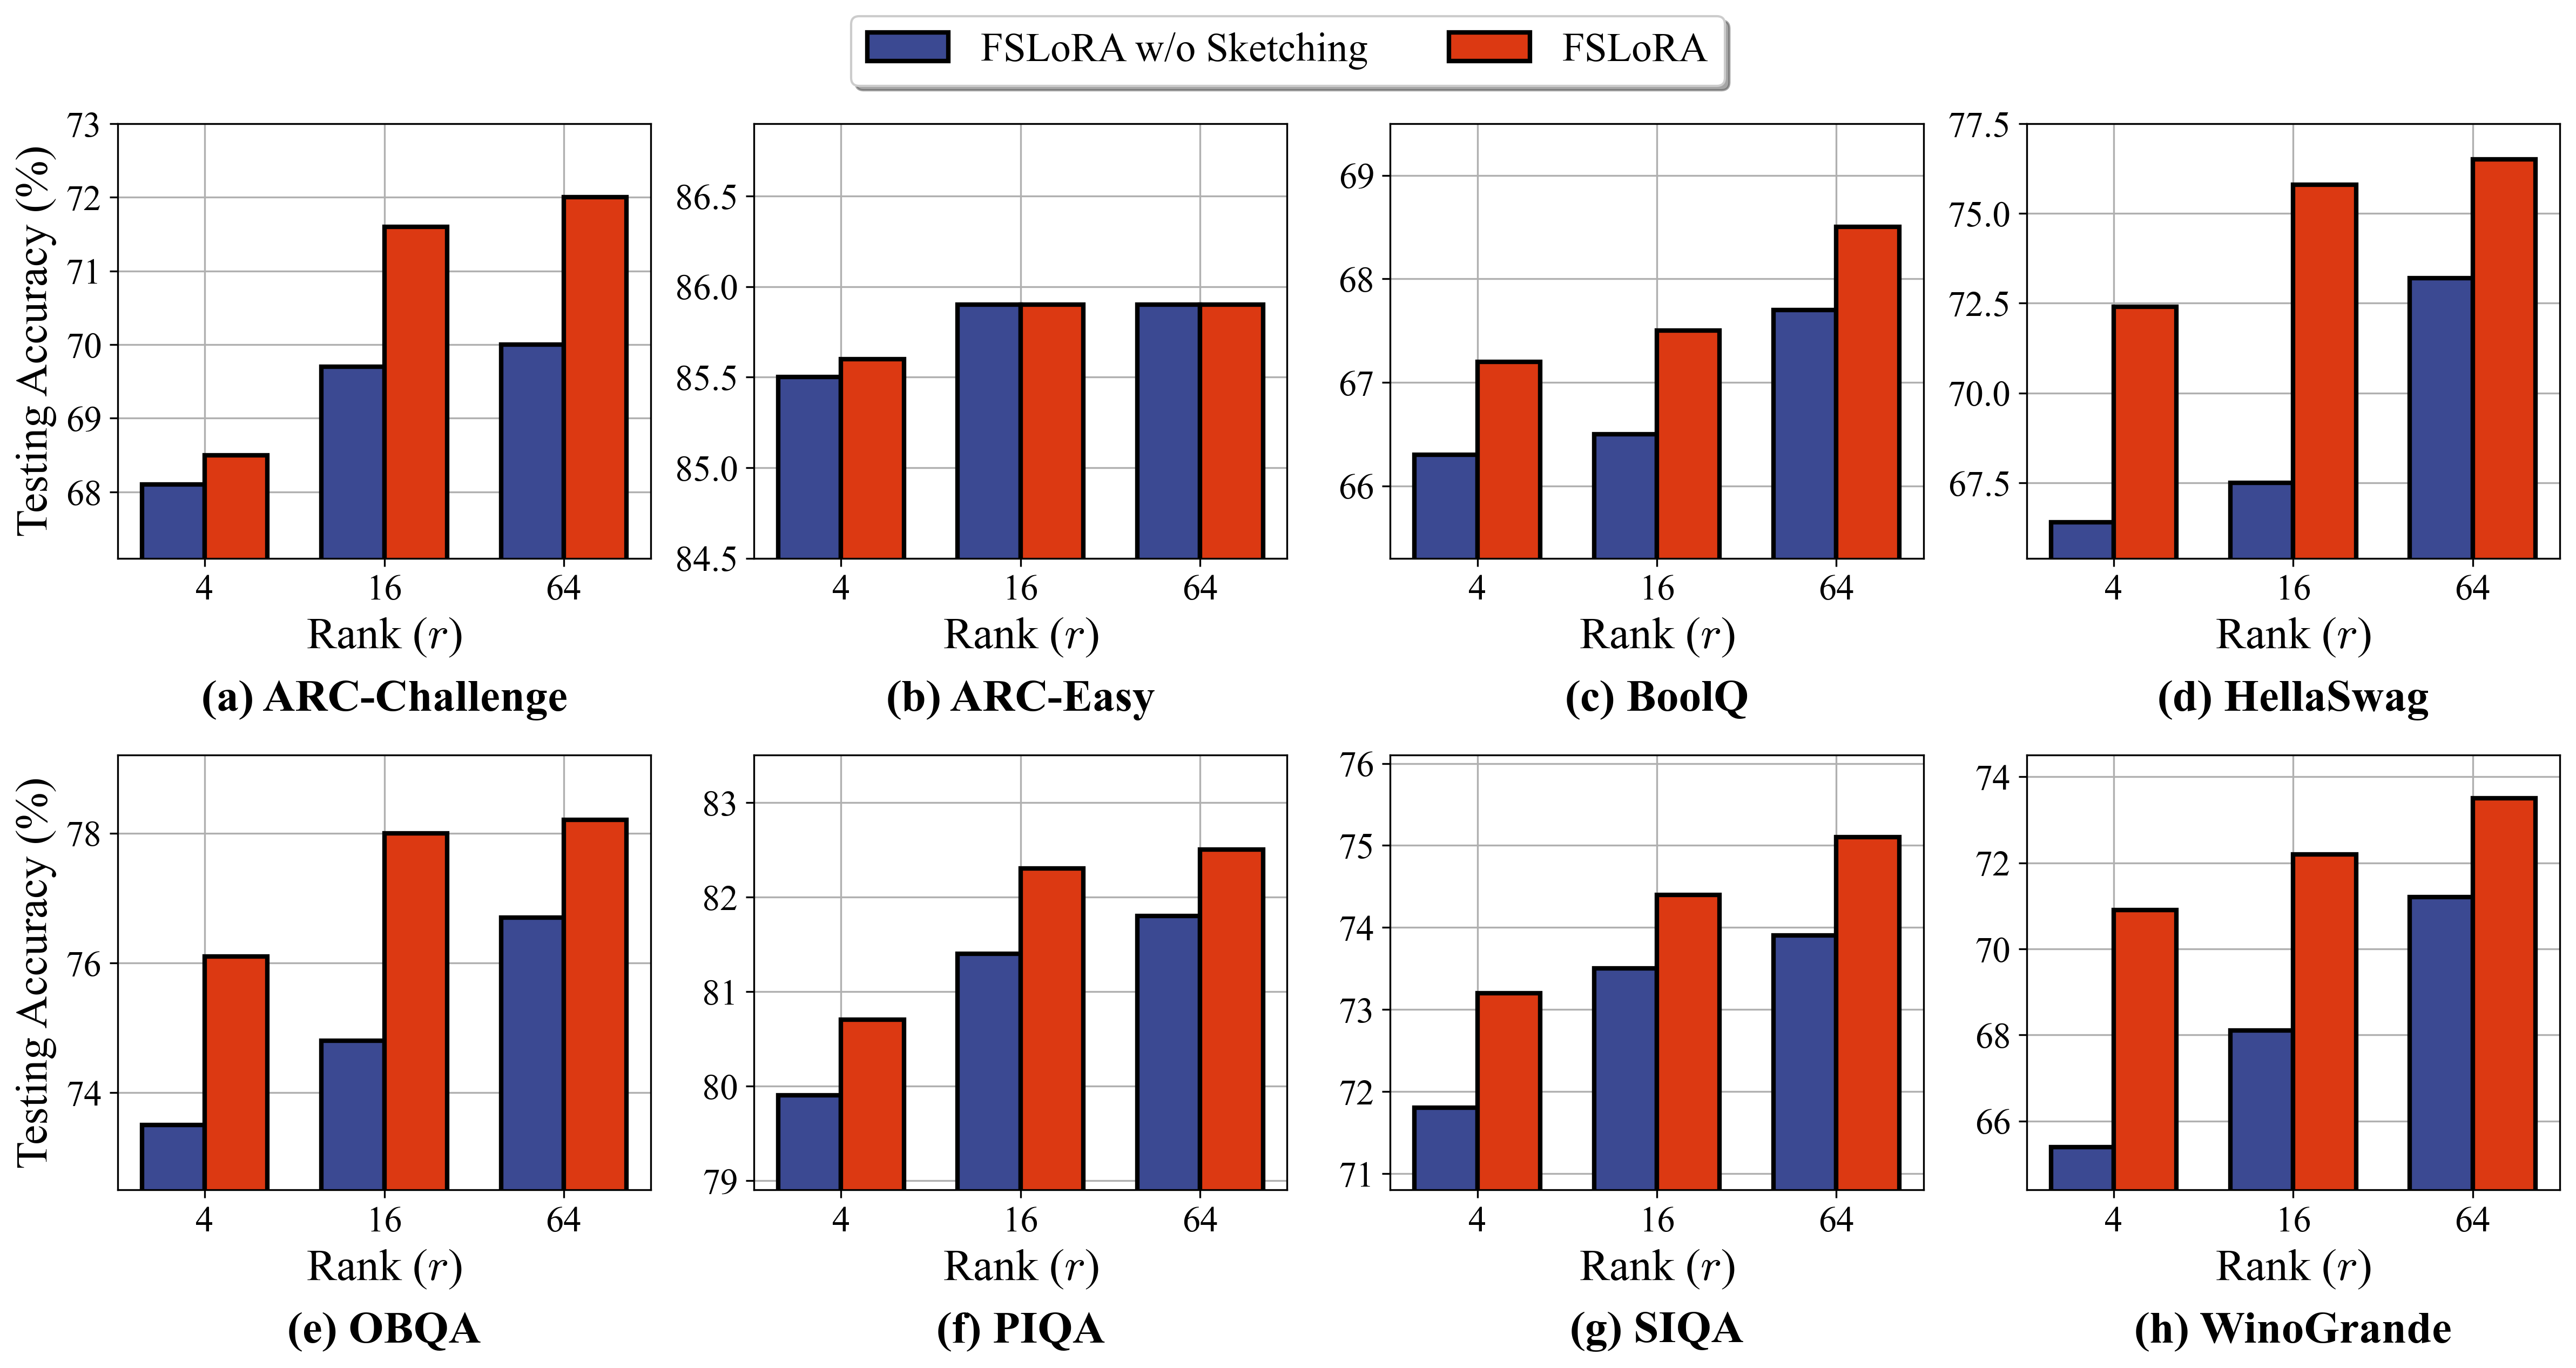
\includegraphics[width=\linewidth]{Figure/More_Device_50_detail.png}
    \caption{Comparison of FSLoRA with and without sketching, with an upload budget \(200 \times\) the global LoRA module size at each rank, evaluated on the commonsense reasoning benchmark and the LLaMA-3.2-3B model. The number of devices is set to \(50\).
    We observe that the sketching mechanism improves performance across all considered tasks. The average accuracy of the eight tasks is shown in Figure \ref{fig:more_device_average}.}
    \label{fig:more_device}
\end{figure}
\begin{figure}[h!]
    \centering
    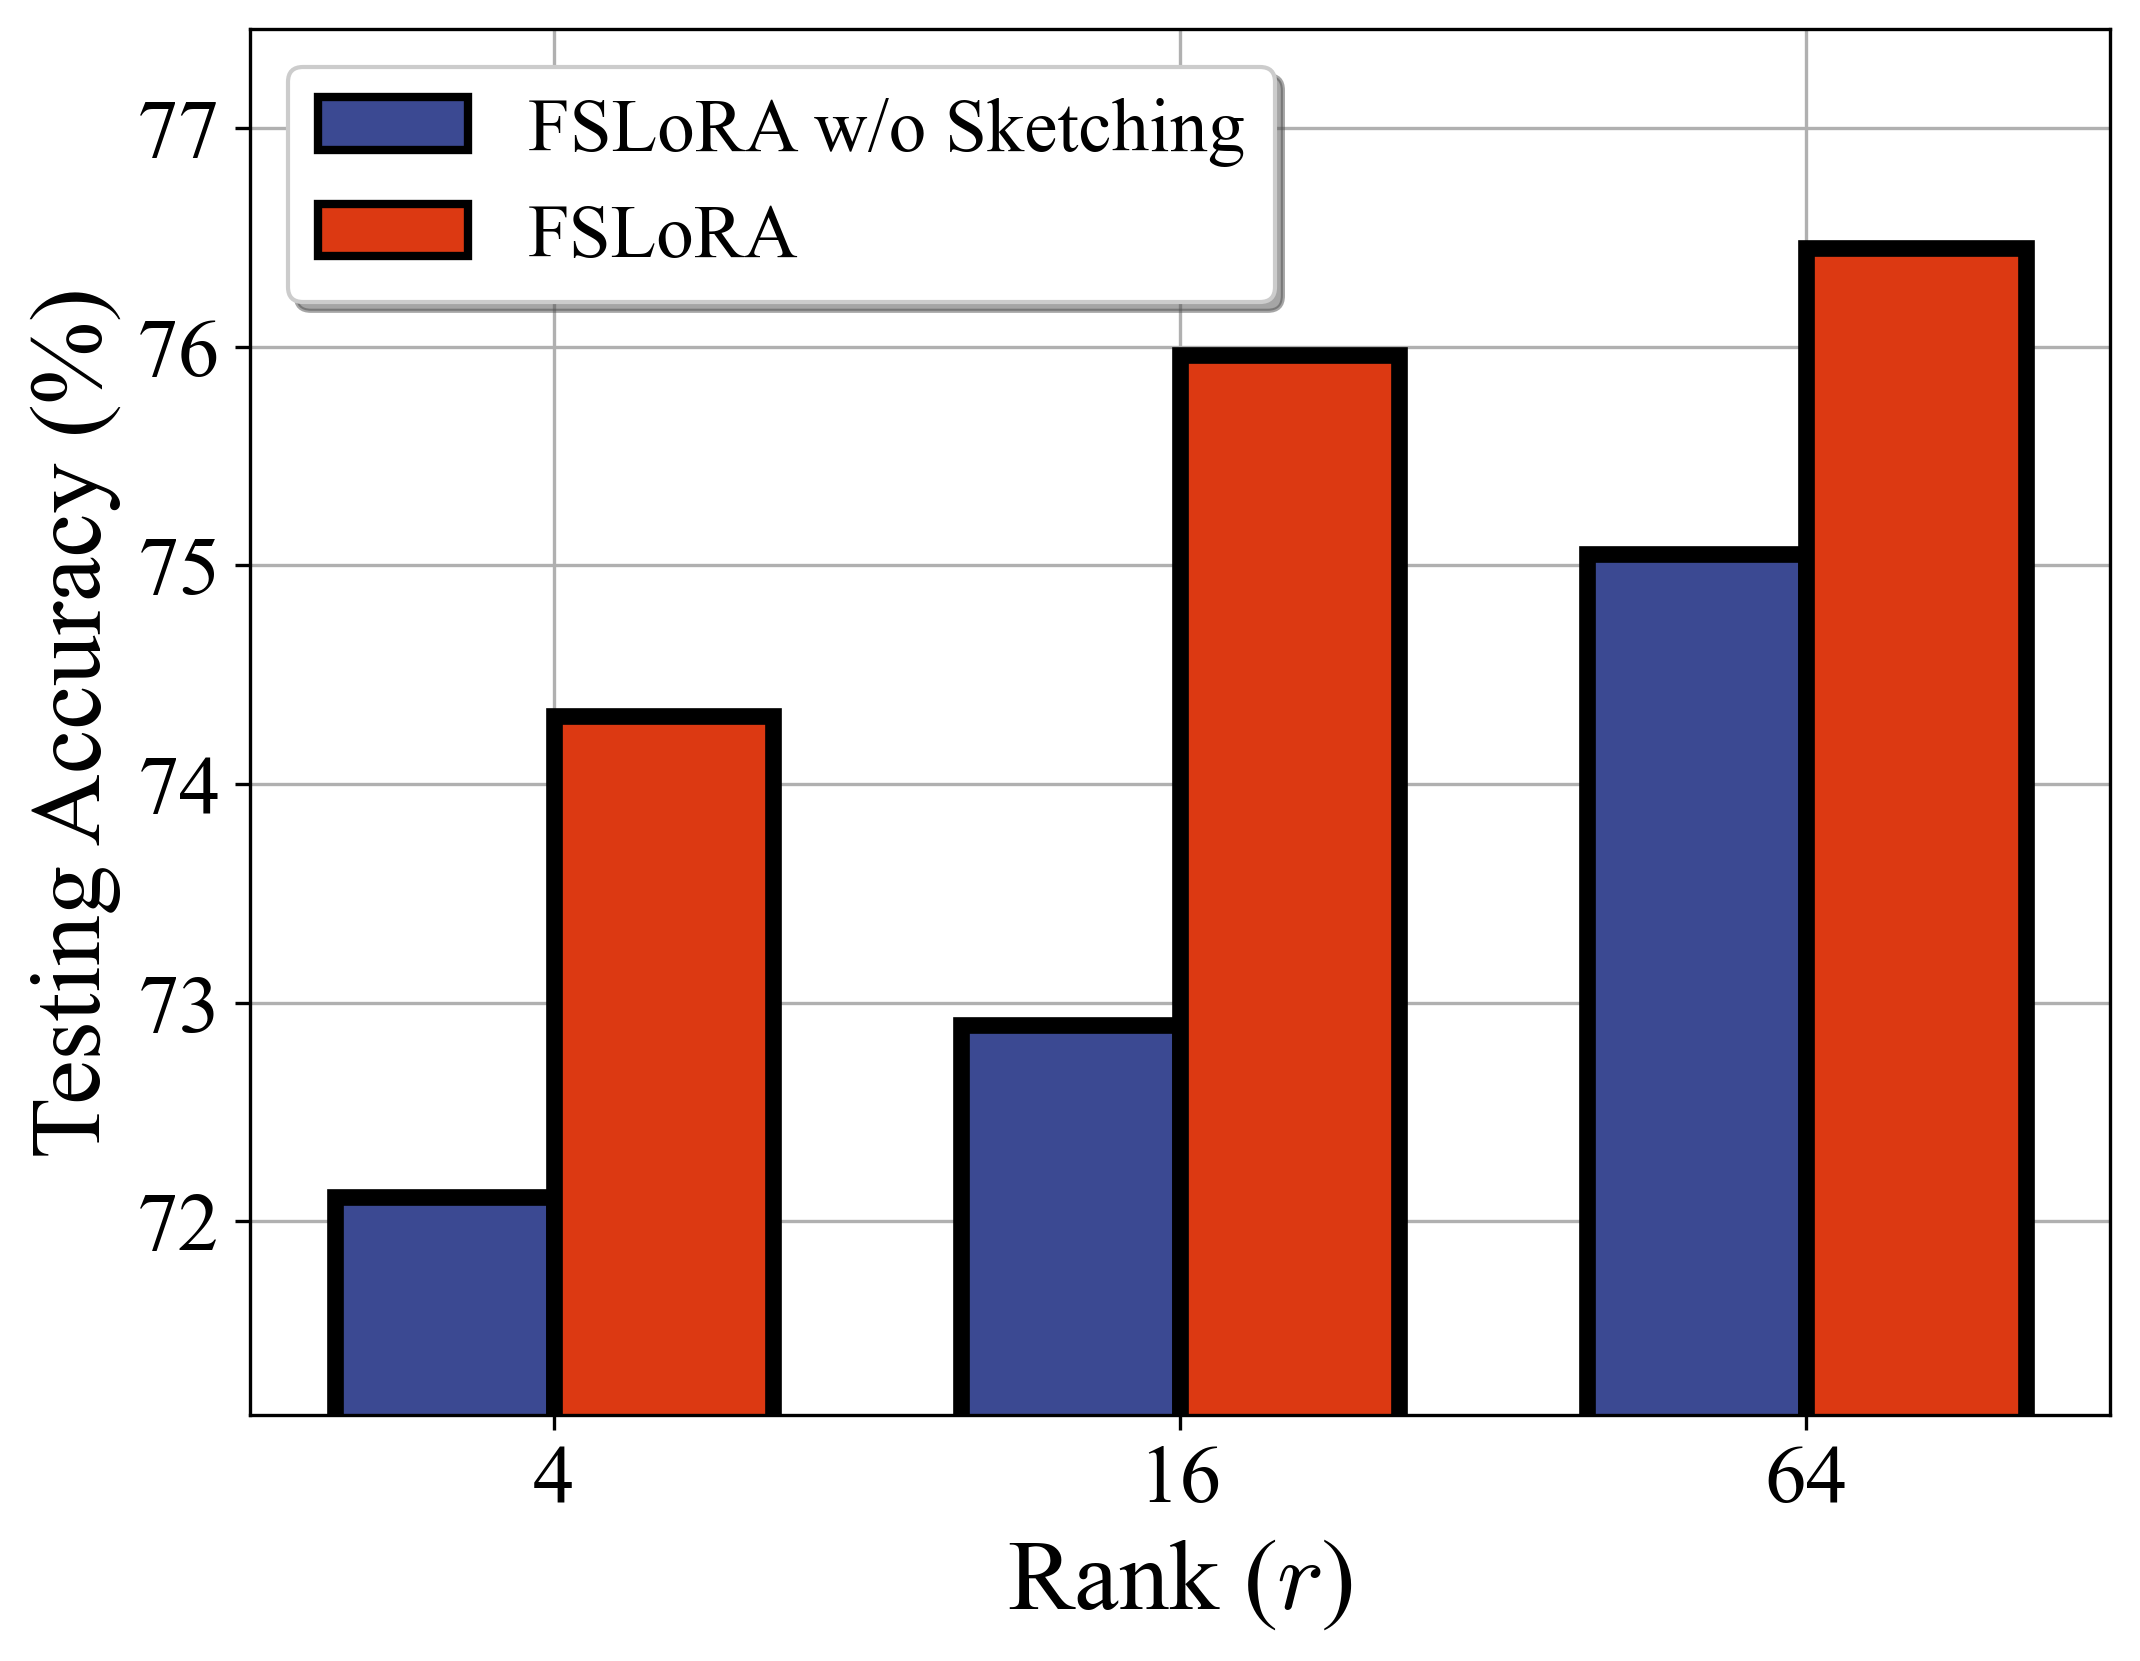
\includegraphics[width=0.4\linewidth]{Figure/More_Device_50.png}
    \caption{Comparison of FSLoRA with and without sketching, with an upload budget \(200 \times\) the global LoRA module size at each rank, evaluated on the LLaMA-3.2-3B model. The number of devices is set to \(50\). The results are averaged over eight tasks from the commonsense reasoning benchmark.}
    \label{fig:more_device_average}
\end{figure}
\end{comment}



\section{Implementation Details}
\label{appen:implementation_details}
\subsection{Details on Hyperparameters}
%\label{appen:hyperparameters}
Unless stated otherwise, the hyperparameters used in this work are as follows.
\begin{table}[H]
\caption{
The hyperparameters for RoBERTa \& GLUE and LLaMA-3.2-3B \& commonsense reasoning benchmarks.
}
\label{tab:hyperparameters}

\centering
\resizebox{\linewidth}{!}{
\begin{tabular}{l|cc}
    \toprule
    Hyperparameter & RoBERTa \& GLUE & LLaMA-3.2-3B \& commonsense reasoning \\
   \midrule
   Dirichlet parameter & 0.1 & 0.1 \\
   \midrule
    Batch size & 16 & 16 \\
    \midrule
   LoRA dropout rate & 0.1 & 0.1 \\ %\multicolumn{2}{c}{0.1}
    \midrule
    Learning rate, $\gamma$ & 5e-4 & 3e-4 \\
    \midrule
    Communication round, $T$ & 200 & 200 \\
    \midrule
    Local iteration number, $H$& 50 & 20 \\
    \midrule
    % Number of edge devices, $N$& 20 & 20 \\
    % \midrule
    Target module  & [``query'', ``value'', ``classification head''] & [``q\_proj'', ``k\_proj'', ``v\_proj'', ``up\_proj'', ``down\_proj''] \\
    \bottomrule
\end{tabular}
}
\end{table}

%\newpage

\subsection{Details on Datasets}
%\label{appen:benchmarks}

\subsubsection{GLUE Benchmark}
GLUE is a widely recognized benchmark designed to assess the natural language understanding capabilities of language models \citep{wang2018glue}.
\begin{itemize}[topsep=0pt,itemsep=4pt,parsep=0pt, partopsep=0pt, leftmargin=*]
    \item \textbf{CoLA} focuses on whether a given sentence is acceptable according to linguistic rules. It evaluates a model's ability to recognize well-formed sentences.
    \begin{itemize}
        \item[$\rhd$] Input: A single sentence.
        \item[\ding{73}] Output: A label indicating whether the sentence is acceptable or unacceptable.
    \end{itemize}
    \item \textbf{SST-2} is designed for sentiment classification on movie reviews or short texts. It tests whether a model can correctly identify positive or negative sentiment in a given sentence.
    \begin{itemize}
        \item[$\rhd$] Input: A single sentence. 
        \item[\ding{73}] Output: A label indicating positive or negative sentiment.
    \end{itemize}
    \item \textbf{MRPC} checks if two sentences are paraphrases of each other, i.e., if they mean the same thing.
    \begin{itemize}
        \item[$\rhd$] Input: Two sentences (`sentence1' and `sentence2'). 
        \item[\ding{73}] Output: A label indicating either equivalent or not equivalent. 
    \end{itemize}
    \item \textbf{QQP} tests a model's ability to determine if two questions ask the same thing.
    \begin{itemize}
        \item[$\rhd$] Input: Two questions. 
        \item[\ding{73}] Output: A label indicating duplicate or not duplicate.
    \end{itemize}
    \item \textbf{MNLI} tests whether a given hypothesis is entailed, contradicted, or neutral with respect to a premise. 
    \begin{itemize}
        \item[$\rhd$] Input: A premise (first sentence) and a hypothesis (second sentence). 
        \item[\ding{73}] Output: A label indicating entailment, contradiction, or neutral.
    \end{itemize}
    \item \textbf{QNLI} aims to determine if a context sentence correctly answers a given question. 
    \begin{itemize}
        \item[$\rhd$] Input: A question and a sentence.  
        \item[\ding{73}] Output: A label indicating the sentence answers the question or it does not.
    \end{itemize}
    \item \textbf{RTE} provides pairs of sentences to see if one implies the other. 
    \begin{itemize}
        \item[$\rhd$] Input: Two sentences (`sentence1' and `sentence2')
        \item[\ding{73}] Output: A label indicating whether the meaning of one sentence is entailed from the other one.
    \end{itemize}
\end{itemize}

%\newpage

\subsubsection{Commonsense Reasoning Benchmark}
The training set of the commonsense reasoning benchmark is a mixture of multiple datasets including about 170K training samples from ARC-c/e \citep{clark2018think}, BoolQ \citep{clark2019boolq}, HellaSwag \citep{zellers2019hellaswag}, OBQA \citep{mihaylov2018can}, PIQA \citep{bisk2020piqa}, SIQA \citep{sap2019socialiqa}, and WinoGrande \citep{sakaguchi2021winogrande} datasets. 
\begin{itemize}[leftmargin=*]
    \item \textbf{ARC-c/e} contains the challenge and easy question set from the ARC dataset of genuine grade-school level, multiple-choice science questions.
    \item \textbf{BoolQ} is a question-answering dataset with yes/no questions derived from natural, real-world scenarios. 
    \item \textbf{HellaSwag} includes questions for commonsense natural language inference, where a context and multiple endings are given, requiring the most coherent ending to be selected.
    \item \textbf{OBQA} involves multi-step problem-solving that combines commonsense knowledge, reasoning, and comprehension of accompanying textual information.
    \item \textbf{PIQA} focuses on questions requiring physical commonsense to solve. Each question offers two answer choices. 
    \item \textbf{SIQA} targets reasoning about human actions and their social implication. 
    \item \textbf{WinoGrande} is designed as a binary-choice fill-in-the-blank task, this dataset evaluates the ability to resolve ambiguous sentences through commonsense reasoning.
\end{itemize}
The input template, i.e., prompt format for these datasets is detailed in Table \ref{tab:input_template}.

\begin{table}[H]
\caption{The prompt template of the commonsense reasoning datasets \citep{hu2023llm}.}
\label{tab:input_template}

\begin{tabularx}{\textwidth}{lX}
\toprule
Dataset & Input Template \\
\midrule


ARC-c/e & 
\begin{minipage}{\linewidth}
\begin{tcolorbox}[colback=gray!10,colframe=black!75!black, left=1mm, right=1mm, top=1mm, bottom=1mm]
Please choose the correct answer to the question: [QUESTION] 

Answer1: [ANSWER\_1]

Answer2: [ANSWER\_2]

Answer3: [ANSWER\_3]

Answer4: [ANSWER\_4]

Answer format: answer1/answer2/answer3/answer4

the correct answer is [ANSWER]
\end{tcolorbox}
\end{minipage} \\
\midrule


BoolQ & 
\begin{minipage}{\linewidth}
\begin{tcolorbox}[colback=gray!10,colframe=black!75!black, left=1mm, right=1mm, top=1mm, bottom=1mm]
Please answer the following question with true or false, question: [QUESTION]

Answer format: true/false

the correct answer is [ANSWER]
\end{tcolorbox}
\end{minipage} \\
\midrule


HellaSwag & 
\begin{minipage}{\linewidth}
\begin{tcolorbox}[colback=gray!10,colframe=black!75!black, left=1mm, right=1mm, top=1mm, bottom=1mm]
Please choose the correct ending to complete the given sentence: [ACTIVITY\_LABEL]: [CONTEXT]

Ending1: [ENDING\_1] 

Ending2: [ENDING\_2] 

Ending3: [ENDING\_3] 

Ending4: [ENDING\_4] 

Answer format: ending1/ending2/ending3/ending4 

the correct answer is [ANSWER]
\end{tcolorbox}
\end{minipage} \\
\midrule


OBQA & 
\begin{minipage}{\linewidth}
\begin{tcolorbox}[colback=gray!10,colframe=black!75!black, left=1mm, right=1mm, top=1mm, bottom=1mm]
Please choose the correct answer to the question: [QUESTION] 

Answer1: [ANSWER\_1]

Answer2: [ANSWER\_2]

Answer3: [ANSWER\_3]

Answer4: [ANSWER\_4]

Answer format: answer1/answer2/answer3/answer4

the correct answer is [ANSWER]
\end{tcolorbox}
\end{minipage} \\
\midrule


PIQA & 
\begin{minipage}{\linewidth}
\begin{tcolorbox}[colback=gray!10,colframe=black!75!black, left=1mm, right=1mm, top=1mm, bottom=1mm]
Please choose the correct solution to the question: [QUESTION]

Solution1: [SOLUTION\_1]

Solution2: [SOLUTION\_2]

Answer format: solution1/solution2 

the correct answer is [ANSWER]
\end{tcolorbox}
\end{minipage} \\
\midrule


SIQA & 
\begin{minipage}{\linewidth}
\begin{tcolorbox}[colback=gray!10,colframe=black!75!black, left=1mm, right=1mm, top=1mm, bottom=1mm]
Please choose the correct answer to the question: [QUESTION]

Answer1: [ANSWER\_1]

Answer2: [ANSWER\_2]

Answer3: [ANSWER\_3]

Answer format: answer1/answer2/answer3 

the correct answer is [ANSWER]
\end{tcolorbox}
\end{minipage} \\
\midrule


WinoGrande & 
\begin{minipage}{\linewidth}
\begin{tcolorbox}[colback=gray!10,colframe=black!75!black, left=1mm, right=1mm, top=1mm, bottom=1mm]
Please choose the correct answer to fill in the blank to complete the given sentence: [SENTENCE]

Option1: [OPTION\_1]

Option2: [OPTION\_2]

the correct answer is [ANSWER]
\end{tcolorbox}
\end{minipage} \\
\bottomrule

\end{tabularx}
\end{table}

\section{Proof of the Theoretical Results}
\subsection{Preliminaries}
Before presenting the proof of the main results, we first introduce some preliminary facts that will be used later. Throughout this work, $\|\cdot\|$ denotes the Frobenius norm when applied to a matrix and the $\ell_2$ norm when applied to a vector.

\begin{lemma}\label{pre:lemma:variable:0}
    Suppose a sequence of independent random matrices $\left\{{\bf P}_i\right\}_{i=1}^N$ satisfy $\mathbb{E}[{\bf P}_i] = {\bf 0}, \forall i.$ Then, $$\mathbb{E}\left\|\frac{1}{N} \sum_{i=1}^N {\bf P}_i\right\|^2 = \frac{1}{N^2} \sum_{i=1}^N \mathbb{E} \left\|{\bf P}_i\right\|^2.$$
\end{lemma}

\begin{lemma} {\normalfont \citep[Lemma 2]{jianyu}}\label{pre:lemma:jianyu}
Suppose a sequence of random matrices $\left\{{\bf P}_i\right\}_{i=1}^N$ satisfy $\mathbb{E} \left[{\bf P}_i \mid {\bf P}_{i-1}, \!{\bf P}_{i-2}, \ldots, {\bf P}_1 \right]={\bf 0}, \forall i.$ Then,
$$
\mathbb{E}\left[\left\|\sum_{i=1}^N {\bf P}_i\right\|^2\right]=\sum_{i=1}^N \mathbb{E}\left[\left\|{\bf P}_i\right\|^2\right] .
$$
\end{lemma}

\begin{lemma}\label{lemma:tune_stepsize}
{\normalfont \citep[Lemma 17]{koloskova2020unified}}\label{converging_iterates} For any $a_0 \geq 0, b\geq 0, c\geq 0, d >0$, there exist a constant $\eta \leq \frac{1}{d}$ such that
\begin{align}
\frac{a_0}{T \eta } + b \eta + c \eta^2 \leq 2 \left( \frac{a_0 b}{T} \right)^{\frac{1}{2}} + 2 c^{\frac{1}{3}} \left(\frac{a_0}{T}\right)^{\frac{2}{3}} + \frac{d a_0}{T}.
\end{align}
\end{lemma}

\begin{lemma}[Random sketching bounds]\label{lamma:sketching_bound}
Let $\mathbf{S}$ be a random diagonal sketching matrix of the form
\[
\mathbf{S}
\;=\;
\frac{r}{k}\,\sum_{j \in \mathcal{I}} \mathbf{e}_j\,\mathbf{e}_j^{\top},
\]
where \(\mathbf{e}_1, \dots, \mathbf{e}_r \in \mathbb{R}^r\) are standard unit basis vectors and $\mathcal{I}\subseteq \{1,\dots,r\}$ is chosen uniformly at random with $|\mathcal{I}|=k$. Then any matrix $\mathbf{X}$ we have
\begin{equation}\label{diag:worstcase_bound}
\|\mathbf{X}\,\mathbf{S}\|^{2}
~\le~
\frac{r^{2}}{k^{2}}
\,\|\mathbf{X}\|^{2},
\end{equation}
and in expectation we have
\begin{equation}\label{diag:expected_bound}
\mathbb{E}_{\mathbf{S}}\!\Bigl[\|\mathbf{X}\,\mathbf{S}\|^{2}\Bigr]
~\le~
\frac{r}{k}
\,\|\mathbf{X}\|^{2}.
\end{equation}
\end{lemma}

\begin{proof}
Since $\mathbf{S}$ is diagonal with exactly $k$ diagonal entries equal to $\tfrac{r}{k}$ and the rest zero, its largest eigenvalue is $\tfrac{r}{k}$.  Squaring gives
\[
\mathbf{S}\,\mathbf{S}^{\!\top}
~=~
\mathbf{S}^{2}
~\preceq~
\frac{r^{2}}{k^{2}}
\,\mathbf{I},
\]
Equivalently,
\[
\mathbf{x}^{\top}
\bigl(\mathbf{S}\,\mathbf{S}^{\!\top}\bigr)
\mathbf{x}
~\le~
\frac{r^{2}}{k^{2}}
\,\|\mathbf{x}\|^{2},
 \forall \mathbf{x}.
\]
Setting $\mathbf{x} = \mathbf{x}_j$ to be the $j$-th column of $\mathbf{X}$ and summing over $j$ implies
\[
\|\mathbf{X}\,\mathbf{S}\|^{2}
~
=\;
\sum_{j}
\,\|\mathbf{S}^{\!\top}\,\mathbf{x}_j\|^{2}
~
=\;
\sum_{j}
\,\mathbf{x}_j^{\top}
\,(\mathbf{S}\,\mathbf{S}^{\!\top})
\,\mathbf{x}_j
~\le~
\frac{r^{2}}{k^{2}}
\,\sum_{j}
\,\|\mathbf{x}_j\|^{2}
~
=\;
\frac{r^{2}}{k^{2}}
\,\|\mathbf{X}\|^{2},
\]
which proves~\eqref{diag:worstcase_bound}.

For the expected bound~\eqref{diag:expected_bound}, note that each diagonal index $j\in\{1,\dots,r\}$ is included in $\mathcal{I}$ with probability $\tfrac{k}{r}$.  Hence the expectation of $\mathbf{S}^{2}$ satisfies
\[
\mathbb{E}_{\mathbf{S}}\bigl[\mathbf{S}^{2}\bigr]
~
=\;
\frac{r^{2}}{k^{2}}
\,\mathbb{E}\Bigl[\sum_{j\in \mathcal{I}} \mathbf{e}_j\,\mathbf{e}_j^{\top}\Bigr]
~
=\;
\frac{r^{2}}{k^{2}}
\,
\frac{k}{r}\,\mathbf{I}
~
=\;
\frac{r}{k}\,\mathbf{I}.
\]
Thus for any vector $\mathbf{x}$,
\[
\mathbb{E}_{\mathbf{S}}
\!\Bigl[\|\mathbf{S}^{\!\top}\mathbf{x}\|^{2}\Bigr]
~
=\;
\mathbb{E}_{\mathbf{S}}
\!\Bigl[\mathbf{x}^{\top}\,\mathbf{S}\,\mathbf{S}^{\!\top}\,\mathbf{x}\Bigr]
~
=\;
\mathbf{x}^{\top}
\Bigl(\mathbb{E}[\mathbf{S}^{2}]\Bigr)
\mathbf{x}
~
=\;
\frac{r}{k}\,\|\mathbf{x}\|^{2}.
\]
Summing over columns of $\mathbf{X}$ again establishes
\[
\mathbb{E}_{\mathbf{S}}
\!\bigl[\|\mathbf{X}\,\mathbf{S}\|^{2}\bigr]
~
=\;
\sum_{j}
\,\mathbb{E}_{\mathbf{S}}
\!\bigl[\|\mathbf{S}^{\!\top}\mathbf{x}_j\|^{2}\bigr]
~
=\;
\sum_{j}
\,\mathbf{x}_j^{\top}
\Bigl(\mathbb{E}[\mathbf{S}^{2}]\Bigr)
\mathbf{x}_j
~
=\;
\frac{r}{k}
\,\|\mathbf{X}\|^{2}.
\]
This completes the proof of Lemma \ref{lamma:sketching_bound}.
\end{proof}

\subsection{Proof of Lemma \ref{compute_grad}}\label{proof_compute_grad}
From the chain rule for matrix calculus, we know that: 
    \[\nabla_{\bf Y} g({\bf X}{\bf Y}) ={\bf X}^{\top} \nabla g({\bf X}{\bf Y}), ~\nabla_{\bf X} g({\bf X}{\bf Y}) =  \nabla g({\bf X} {\bf Y}){\bf Y}^{\top}, \]
    %$\nabla_{\bf Y} g({\bf X}{\bf Y}) ={\bf X}^{\top} \nabla g(\bf X{\bf Y}) $ and $\nabla_{\bf X} g({\bf X}{\bf Y}) =  \nabla g({\bf X} {\bf Y}){\bf Y}^{\top}$, 
    where \(\nabla g({\bf X} {\bf Y})\) denotes the gradient of \(g\) to \({\bf X} {\bf Y}\). Applying this to \(\ell({\bf W}_0 + {\bf B} {\bf S} {\bf A}, \xi)\), %we can derive its gradient with respect to \(\bf B\) by setting \({\bf Y} = \bf S{\bf A}\) and \(\bf X = \bf B\). Similarly, we can obtain its gradient to \(\bf A\) by setting \(\bf X = {\bf B}\bf S\) and \({\bf Y} ={\bf A}\). 
    we proceed as follows: \\
    To compute the gradient with respect to \(\mathbf{B}\), set \({\bf X} = \mathbf{B}\) and \({\bf Y} = \mathbf{S}\mathbf{A}\):
   \[
   \nabla_{\mathbf{B}} \ell({\bf W}_0 + {\bf BSA}, \xi) = \nabla \ell({\bf W}_0 + {\bf BSA}, \xi) (\mathbf{S}\mathbf{A})^\top.
   \]
   Similarly, to compute the gradient with respect to \(\mathbf{A}\), set \({\bf X} = \mathbf{B}\mathbf{S}\) and \({\bf Y} = \mathbf{A}\):
   \[
   \nabla_{\mathbf{A}} \ell({\bf W}_0 + {\bf BSA}, \xi) = \mathbf{S}^\top  \mathbf{B}^\top  \nabla \ell({\bf W}_0 + {\bf BSA}, \xi).
   \]


\subsection{Proof of Theorem \ref{convergence_fed_slora_condense}}\label{proof_theorem}
The proof of Theorem \ref{convergence_fed_slora_condense} relies on the following proposition. 
\begin{proposition}\label{smooth_derivation}
    Under Assumption \ref{smoothness_assumption}, \(\tilde{f}_{i} ({\bf X}; {\bf S}) = f_i({\bf B} {\bf S}, {\bf A}),~{\bf S} \in \mathcal{S}_i \), \(f_i^{\mathcal{S}}({\bf X}) = \mathbb{E}_{{\bf S} \sim \mathcal{S}_i} [\tilde{f}_{i} ({\bf X}; {\bf S}) ]\), and \(f^{\mathcal{S}} ({\bf X}) = \frac{1}{N} \sum_{i=1}^N f_i^{\mathcal{S}}(\mathbf{X})\) are smooth with parameters \(L \frac{r^2}{k_i^2}\), \(L \frac{r}{k_i}\), and \(\left( \frac{1}{N} \sum_{i=1}^N \frac{r}{k_i} \right) L \), respectively. 
\end{proposition}
The proof of Proposition \ref{smooth_derivation} is deferred to Appendix \ref{proof_smooth}. With this proposition, we are ready to prove Theorem \ref{convergence_fed_slora_condense}. 

In FSLoRA, the update direction in \eqref{gradient_client_i} corresponds to the negative stochastic gradient of \(\ell({\bf W}_0 + {\bf B} {\bf S} {\bf A}, \xi)\) with respect to \([{\bf B}; {\bf A}]\) for a given sketch \( {\bf S}_i^t\).
We have defined \(\tilde{\ell} ({\bf X}, \xi; {\bf S}) = \ell({\bf W}_0 + {\bf B}{\bf S}{\bf A}, \xi)\). The iterative equation for the proposed FSLoRA algorithm thus can be written as
\begin{equation}
   {\bf X}^{t+1} ={\bf X}^{t} - \gamma \frac{1}{N} \sum_{i=1}^{N} \sum_{h=0}^{H-1} \nabla_{\bf X} \tilde{\ell} ({\bf X}^{t,h}_i, \xi_i^{t,h}; {\bf S}_i^t),
\end{equation}
where \({\bf g}^{t,h}_i\) denotes the stochastic gradient \(\nabla_{\bf X} \tilde{\ell} ({\bf X}^{t,h}_i, \xi_i^{t,h}; {\bf S}_i^t)\).
Based on the smoothness of $f^{\mathcal{S}}(\bf X)$, i.e., Proposition \ref{smooth_derivation}, we have
\begin{align}\label{expansion_smooth}
   \mathbb{E} [f^{\mathcal{S}}({\bf X}^{t+1})] \leq \mathbb{E}[f^{\mathcal{S}}({\bf X}^t)] \underbrace{-\mathbb{E}\left \langle
    \nabla_{\bf X} f^{\mathcal{S}} ({\bf X}^t) , \gamma \frac{1}{N} \sum_{i=1}^{N} \sum_{h=0}^{H-1} {\bf g}^{t,h}_i
    \right \rangle}_{T_1} +
    \frac{\gamma^2 \bar{L}}{2} \underbrace{ \mathbb{E}\left \| \frac{1}{N} \sum_{i=1}^{N} \sum_{h=0}^{H-1}{\bf g}^{t,h}_i \right \|^2}_{T_2},
\end{align}
%where \(\nabla_{\bf X} f^{\mathcal{S}}({\bf X}^t)\) denote the gradient of global empirical loss at \({\bf X}^t\).
where \(\bar{L} = \left( \frac{1}{N} \sum_{i=1}^N \frac{r}{k_i} \right) L \).


For \(T_1\), we have 
\begin{align}
    T_1 =& -H\mathbb{E}\left \langle
    \nabla_{\bf X} f^{\mathcal{S}} ({\bf X}^t), \gamma \frac{1}{NH} \sum_{i=1}^{N} \sum_{h=0}^{H-1} {\bf g}^{t,h}_i
    \right \rangle \nonumber \\
    %=& -H\mathbb{E} \left \langle \nabla_{\bf X} f^{\mathcal{S}} ({\bf X}^t), \gamma \frac{1}{N} \sum_{i=1}^{N} \sum_{h=0}^{H-1} \nabla_{\bf X} \tilde{f}_i ({\bf X}_i^{t,h}; {\bf S}_i^t) \right \rangle \nonumber\\
    =& -H\mathbb{E} \left \langle
    \nabla_{\bf X} f^{\mathcal{S}} ({\bf X}^t), \gamma \frac{1}{NH} \sum_{i=1}^{N} \sum_{h=0}^{H-1} \nabla_{\bf X} f_i^{\mathcal{S}} ({\bf X}_i^{t,h})
    \right \rangle \nonumber\\
    =&  -\frac{\gamma H}{2} \mathbb{E} \left\| \nabla_{\bf X} f^{\mathcal{S}} ({\bf X}^t) \right\|^2 - \frac{\gamma H}{2} \mathbb{E} \left\| \frac{1}{NH} \sum_{i=1}^{N} \sum_{h=0}^{H-1} \nabla_{\bf X} f_i^{\mathcal{S}} ({\bf X}_i^{t,h}) \right\|^2
    \nonumber\\
    & + \frac{\gamma H}{2} \mathbb{E} \left \|
    \nabla_{\bf X} f^{\mathcal{S}} ({\bf X}^t) - \frac{1}{NH} \sum_{i=1}^{N} \sum_{h=0}^{H-1} \nabla_{\bf X} f_i^{\mathcal{S}} ({\bf X}_i^{t,h}) 
    \right \|^2 \nonumber\\
    \leq&  - \frac{\gamma H}{2} \mathbb{E} \left\| \nabla_{\bf X} f^{\mathcal{S}} ({\bf X}^t) \right\|^2 - \frac{\gamma H}{2} \mathbb{E} \left\| \frac{1}{N} \sum_{i=1}^{N} \sum_{h=0}^{H-1} \nabla_{\bf X} f_i^{\mathcal{S}} ({\bf X}_i^{t,h}) \right\|^2
    \nonumber\\
    & + \frac{\gamma}{2} \sum_{h=0}^{H-1} \mathbb{E} \left \|\frac{1}{N} \sum_{i=1}^{N} \nabla_{\bf X} f_i^{\mathcal{S}} ({\bf X}^t) - \frac{1}{N} \sum_{i=1}^{N} \nabla_{\bf X} f_i^{\mathcal{S}} ({\bf X}_i^{t,h}) 
    \right \|^2 \nonumber\\
    \leq&  - \frac{\gamma H}{2} \mathbb{E} \left\| \nabla_{\bf X} f^{\mathcal{S}} ({\bf X}^t) \right\|^2 - \frac{\gamma }{2H} \mathbb{E} \left\| \frac{1}{N} \sum_{i=1}^{N} \sum_{h=0}^{H-1} \nabla_{\bf X} f_i^{\mathcal{S}} ({\bf X}_i^{t,h}) \right\|^2 \nonumber \\
    & + \frac{\gamma H L^2}{2}  \frac{1}{NH} \sum_{i=1}^{N} \frac{r^2}{k_i^2} \sum_{h=0}^{H-1} \mathbb{E} \left \|{\bf X}_i^{t,h} -{\bf X}^t
    \right \|^2, \label{T_1}
\end{align}
where the last inequalities follow Jensen's inequality and Proposition \ref{smooth_derivation}. 
\begin{comment}
For \(T_2\), we have
\begin{align}
    & \mathbb{E}\left \| \frac{1}{N} \sum_{i=1}^{N} \sum_{h=0}^{H-1} {\bf g}^{t,h}_i \right \|^2 \nonumber\\
    =& \mathbb{E}\left \| \frac{1}{N} \sum_{i=1}^{N} \sum_{h=0}^{H-1} {\bf g}^{t,h}_i \mp  \frac{1}{N} \sum_{i=1}^{N} \sum_{h=0}^{H-1} \nabla_{\bf X} \tilde{f}_i ({\bf X}_i^{t,h};{\bf S}_i^t) \mp  \frac{1}{N} \sum_{i=1}^{N} \sum_{h=0}^{H-1} \nabla_{\bf X} f_i^{\mathcal{S}} ({\bf X}_i^{t,h}) \right \|^2 \nonumber\\
    \leq & 3\mathbb{E}\left \| \frac{1}{N} \sum_{i=1}^{N} \sum_{h=0}^{H-1} {\bf g}^{t,h}_i - \frac{1}{N} \sum_{i=1}^{N} \sum_{h=0}^{H-1} \nabla_{\bf X} \tilde{f}_i ({\bf X}_i^{t,h};{\bf S}_i^t) \right \|^2 \nonumber\\
    &+  3\mathbb{E}\left \| \frac{1}{N} \sum_{i=1}^{N} \sum_{h=0}^{H-1} \nabla_{\bf X} \tilde{f}_i ({\bf X}_i^{t,h};{\bf S}_i^t) -  \frac{1}{N} \sum_{i=1}^{N} \sum_{h=0}^{H-1} \nabla_{\bf X} f_i^{\mathcal{S}} ({\bf X}_i^{t,h}) \right \|^2 + 3\mathbb{E}\left \| \frac{1}{N} \sum_{i=1}^{N} \sum_{h=0}^{H-1} \nabla_{\bf X} f_i^{\mathcal{S}} ({\bf X}_i^{t,h}) \right \|^2 \nonumber\\
    =& \frac{3}{N^2} \sum_{i=1}^{N} \mathbb{E}\left \|  \sum_{h=0}^{H-1} {\bf g}^{t,h}_i - \sum_{h=0}^{H-1} \nabla_{\bf X} \tilde{f}_i ({\bf X}_i^{t,h};{\bf S}_i^t) \right \|^2 \nonumber\\
    &+ \frac{3}{N^2} \sum_{i=1}^{N} \mathbb{E}\left \| \sum_{h=0}^{H-1} \nabla_{\bf X} \tilde{f}_i ({\bf X}_i^{t,h};{\bf S}_i^t) - \sum_{h=0}^{H-1} \nabla_{\bf X} f_i^{\mathcal{S}} ({\bf X}_i^{t,h}) \right \|^2 + 3\mathbb{E}\left \| \frac{1}{N} \sum_{i=1}^{N} \sum_{h=0}^{H-1} \nabla_{\bf X} f_i^{\mathcal{S}} ({\bf X}_i^{t,h}) \right \|^2 \nonumber\\
    \leq & 3H\frac{\sigma_g^2 + \sigma_s^2}{N} + 3\mathbb{E}\left \| \frac{1}{N} \sum_{i=1}^{N} \sum_{h=0}^{H-1} \nabla_{\bf X} f_i^{\mathcal{S}} ({\bf X}_i^{t,h}) \right \|^2, \label{T_2}
\end{align}
where the last equality comes from Lemma \ref{pre:lemma:variable:0} while the last inequality follows Lemma \ref{pre:lemma:jianyu} and Assumption \ref{varaince_assumption}. 
\end{comment}

For $T_2$, we have
\begin{align}
    T_2 = & \mathbb{E}\left \| \frac{1}{N} \sum_{i=1}^{N} \sum_{h=0}^{H-1} ({\bf g}^{t,h}_i \mp \nabla_{\bf X} f_i^{\mathcal{S}} ({\bf X}_i^{t,h}))\right \|^2 \nonumber\\
    \leq & \frac{2}{N^2} \sum_{i=1}^{N} \mathbb{E}\left \|  \sum_{h=0}^{H-1} ({\bf g}^{t,h}_i -  \nabla_{\bf X} f_i^{\mathcal{S}} ({\bf X}_i^{t,h})) \right \|^2 + 2\mathbb{E}\left \| \frac{1}{N} \sum_{i=1}^{N} \sum_{h=0}^{H-1} \nabla_{\bf X} f_i^{\mathcal{S}} ({\bf X}_i^{t,h}) \right \|^2, \nonumber
\end{align}
where the inequality follows the fact that $\mathbb{E}[\sum_{h=0}^{H-1} ({\bf g}^{t,h}_i -  \nabla_{\bf X} f_i^{\mathcal{S}} ({\bf X}_i^{t,h}))] = 0$ and the independence between clients.

Furthermore, we bound the first term on the right-hand side of the above inequality as
\begin{align}
    \mathbb{E}\left \|  \sum_{h=0}^{H-1} ({\bf g}^{t,h}_i -  \nabla_{\bf X} f_i^{\mathcal{S}} ({\bf X}_i^{t,h})) \right \|^2 = \sum_{h=0}^{H-1} \mathbb{E}\left \|{\bf g}^{t,h}_i -  \nabla_{\bf X} f_i^{\mathcal{S}} ({\bf X}_i^{t,h}) \right \|^2 
    \leq H \sigma^2 + \rho \sum_{h=0}^{H-1} \mathbb{E} \left \|\nabla_{\bf X} f_i^{\mathcal{S}} ({\bf X}_i^{t,h}) \right \|^2, \nonumber
\end{align}
where the equality follows Lemma \ref{pre:lemma:jianyu} and the inequality follows Assumption \ref{varaince_assumption}. 
% We thus obtain
% \begin{align}
%     T_2 \leq  2H\frac{\sigma^2}{N} + \frac{2 \rho}{N^2} \sum_{i=1}^{N} \sum_{h=0}^{H-1} \mathbb{E} \left \|\nabla_{\bf X} f_i^{\mathcal{S}} ({\bf X}_i^{t,h}) \right \|^2 + 2\mathbb{E}\left \| \frac{1}{N} \sum_{i=1}^{N} \sum_{h=0}^{H-1} \nabla_{\bf X} f_i^{\mathcal{S}} ({\bf X}_i^{t,h}) \right \|^2.
% \end{align}
For $\left \|\nabla_{\bf X} f_i^{\mathcal{S}} ({\bf X}_i^{t,h}) \right \|^2$, utilizing Assumption \ref{assumption:gradient_dissimilarity} and Proposition \ref{smooth_derivation}, we have
\begin{align}\label{bound_gradient_i}
& \left \|\nabla_{\bf X} f_i^{\mathcal{S}} ({\bf X}_i^{t,h}) \right \|^2 = \left \|\nabla_{\bf X} f_i^{\mathcal{S}} ({\bf X}_i^{t,h}) \mp \nabla_{\bf X} f_i^{\mathcal{S}} ({\bf X}^{t})  \mp \nabla_{\bf X} f^{\mathcal{S}} ({\bf X}^t)   \right \|^2 \nonumber \\
\leq & 3 \left \|\nabla_{\bf X} f_i^{\mathcal{S}} ({\bf X}_i^{t,h}) - \nabla_{\bf X} f_i^{\mathcal{S}} ({\bf X}^{t}) \right \|^2 + 3 \left \|\nabla_{\bf X} f_i^{\mathcal{S}} ({\bf X}^{t})  - \nabla_{\bf X} f^{\mathcal{S}} ({\bf X}^t)   \right \|^2 + 3 \left \|\nabla_{\bf X} f^{\mathcal{S}} ({\bf X}^t)   \right \|^2 \nonumber \\
\leq & 3 \frac{r^2}{k_i^2} L^2 \left \|{\bf X}_i^{t,h} - {\bf X}^{t} \right \|^2 + 3 (c_h + 1) \| \nabla_{\bf X} f^{\mathcal{S}}({\bf X}^t) \|^2  \!+\! 3 \rho \delta_h^2.
\end{align}
Combining the above three inequalities gives rise to
\begin{align}\label{T_2}
    T_2 
    \leq & \frac{2H}{N} (\sigma^2 + 3 \rho \delta_h^2) + 2\mathbb{E}\left \| \frac{1}{N} \!\sum_{i=1}^{N} \sum_{h=0}^{H-1} \nabla_{\bf X} f_i^{\mathcal{S}} ({\bf X}_i^{t,h}) \right \|^2 + \frac{6\rho (c_h + 1) H}{N} \mathbb{E} \| \nabla_{\bf X} f^{\mathcal{S}}({\bf X}^t) \|^2 \nonumber \\
    &+ \frac{6 \rho H L^2}{N} T_3,
\end{align}
where $T_3 = \frac{1}{NH} \sum_{i=1}^{N} \frac{r^2}{k_i^2} \sum_{h=0}^{H-1} \mathbb{E} \left \|{\bf X}_i^{t,h} -{\bf X}^t
    \right \|^2$.
Combining \eqref{expansion_smooth}, \eqref{T_1}, and \eqref{T_2} yields
\begin{align}
   \mathbb{E} [f^{\mathcal{S}}({\bf X}^{t+1})] \leq & \mathbb{E}[f^{\mathcal{S}}({\bf X}^t)]   - (\frac{\gamma H}{2} - 3\gamma^2 \rho (c_h+1) \frac{H}{N}\bar{L} ) \mathbb{E} \left\| \nabla_{\bf X} f^{\mathcal{S}} ({\bf X}^t) \right\|^2 + \gamma^2 \bar{L} \frac{H}{N} (\sigma^2 + 3\rho \sigma_h^2)
    \nonumber\\
    & - (\frac{\gamma}{2H} -  \gamma^2 \bar{L} ) \mathbb{E} \left\| \frac{1}{N} \sum_{i=1}^{N} \sum_{h=0}^{H-1} \nabla_{\bf X} f_i^{\mathcal{S}} ({\bf X}_i^{t,h}) \right\|^2 
   + (\frac{\gamma H L^2}{2} +  3 \gamma^2 \rho \bar{L} L^2 \frac{H}{N} ) T_3, \nonumber
\end{align}
where \(\bar{L} = \left( \frac{1}{N} \sum_{i=1}^N \frac{r}{k_i} \right) L \).
Let $\gamma \leq \min \{\frac{N}{24 \rho (c_h + 1) H\bar{L}}, \frac{1}{2H\bar{L}}, \frac{N}{6\rho \bar{L}} \}$, we have
\begin{align}\label{T_1_T_2}
   \mathbb{E} [f^{\mathcal{S}}({\bf X}^{t+1})] \leq & \mathbb{E}[f^{\mathcal{S}}({\bf X}^t)]   - \frac{3\gamma H}{8} \mathbb{E} \left\| \nabla_{\bf X} f^{\mathcal{S}} ({\bf X}^t) \right\|^2 + \gamma^2 \bar{L} \frac{H}{N} (\sigma^2 + 3\rho \sigma_h^2)
   + \frac{5\gamma}{8} H L^2 T_3.
\end{align}

For $T_3$, we have
\begin{align}
    T_3 =& \frac{1}{NH} \sum_{i=1}^{N} \frac{r^2}{k_i^2} \sum_{h=0}^{H-1} \mathbb{E} \left \| \gamma \sum_{\tau=0}^{h-1} {\bf g}^{t,\tau}_i
    \right \|^2 \nonumber\\
    =& \gamma^2 \frac{1}{NH} \sum_{i=1}^{N} \frac{r^2}{k_i^2} \sum_{h=0}^{H-1} \mathbb{E} \left \| \sum_{\tau=0}^{h-1} ( {\bf g}^{t,\tau}_i \mp  \nabla_{\bf X} f_i^{\mathcal{S}} ({\bf X}_i^{t,\tau}) )
    \right \|^2 \nonumber\\
    \leq & 2 \gamma^2 \frac{1}{NH} \sum_{i=1}^{N} \frac{r^2}{k_i^2} \sum_{h=0}^{H-1}  \sum_{\tau=0}^{h-1} \mathbb{E} \left \| {\bf g}^{t,\tau}_i - \nabla_{\bf X} f_i^{\mathcal{S}} ({\bf X}_i^{t,\tau})
    \right \|^2 +  2\gamma^2 \frac{1}{NH} \sum_{i=1}^{N} \frac{r^2}{k_i^2} \sum_{h=0}^{H-1} h \sum_{\tau=0}^{h-1} \mathbb{E} \left \|\nabla_{\bf X} f_i^{\mathcal{S}} ({\bf X}_i^{t,\tau})
    \right \|^2 \nonumber\\
    \leq & 2\gamma^2 H \sigma^2 \left( \frac{1}{N} \sum_{i=1}^{N} \frac{r^2}{k_i^2} \right) 
    +  \frac{2 \rho \gamma^2}{NH} \sum_{i=1}^{N} \frac{r^2}{k_i^2} \sum_{h=0}^{H-1}  \sum_{\tau=0}^{h-1} \mathbb{E} \left \|\nabla_{\bf X} f_i^{\mathcal{S}} ({\bf X}_i^{t,\tau})
    \right \|^2 \nonumber \\
    &+ \frac{2\gamma^2}{NH} \sum_{i=1}^{N} \frac{r^2}{k_i^2} \sum_{h=0}^{H-1} h \sum_{\tau=0}^{h-1} \mathbb{E} \left \| \nabla_{\bf X} f_i^{\mathcal{S}} ({\bf X}_i^{t,\tau})
    \right \|^2 \nonumber\\
    \leq & 2\gamma^2 H \sigma^2 \left( \frac{1}{N} \sum_{i=1}^{N} \frac{r^2}{k_i^2} \right) 
    + \frac{2 (\rho+1) \gamma^2 H}{N} \sum_{i=1}^{N} \frac{r^2}{k_i^2} \sum_{h=0}^{H-1} \mathbb{E} \left \| \nabla_{\bf X} f_i^{\mathcal{S}} ({\bf X}_i^{t,\tau})
    \right \|^2. \label{T_3_intermiate_1}
\end{align}

Plugging inequality \eqref{bound_gradient_i} into inequality \eqref{T_3_intermiate_1} yeilds
    \begin{align}
    T_3 \leq & 2 \gamma^2 H \left( \frac{1}{N} \sum_{i=1}^{N} \frac{r^2}{k_i^2} \right) \sigma^2 + 6 (\rho+1) \gamma^2 H^2 \left( \frac{1}{N} \sum_{i=1}^{N} \frac{r^2}{k_i^2} \right) \sigma^2_h  \nonumber \\
    & + 6 (\rho+1) \gamma^2 L^2 H^2 T_3 + 6(\rho+1) \left( \frac{1}{N} \sum_{i=1}^{N} \frac{r^2}{k_i^2} \right) (c_h + 1)\gamma^2 H^2\mathbb{E} \left \| \nabla_{\bf X} f^{\mathcal{S}} ({\bf X}^t)
    \right \|^2.
\end{align}
Denote $\kappa = \frac{1}{N} \sum_{i=1}^{N} \frac{r^2}{k_i^2}$, we simplify the above inequality as 
\begin{align}
    (1- 6(\rho +1) \gamma^2 L^2 H^2) T_3 \leq 2 \kappa \gamma^2 H^2 (\sigma_g^2 + 3(\rho+1) \sigma_h^2) + 6\kappa (\rho+1)(c_h +1) \gamma^2 H^2 \mathbb{E} \left \| \nabla_{\bf X} f^{\mathcal{S}} ({\bf X}^t)  
    \right \|^2. \nonumber
\end{align}
Let $\gamma \leq \frac{1}{\sqrt{12(\rho+1)}HL}$, we get the bound for $T_3$
\begin{align} \label{T_3}
    T_3 \leq 4 \kappa \gamma^2 H^2 (\sigma^2 + 3(\rho+1) \sigma_h^2) + 12 \kappa (\rho+1) (c_h +1) \gamma^2 H^2 \mathbb{E} \left \| \nabla_{\bf X} f^{\mathcal{S}} ({\bf X}^t)
    \right \|^2.
\end{align}
Plugging the bound for $T_3$ into inequality \eqref{T_1_T_2} gives rise to
\begin{align}
   \mathbb{E} [f^{\mathcal{S}}({\bf X}^{t+1})] \leq & \mathbb{E}[f^{\mathcal{S}}({\bf X}^t)]   - ( \frac{3\gamma H}{8} - \frac{5\gamma H}{8} L^2 \left(12 \kappa (\rho+1) (c_h +1) \gamma^2 H^2) \right) \mathbb{E} \left\| \nabla_{\bf X} f^{\mathcal{S}} ({\bf X}^t) \right\|^2 \nonumber \\
   &+ \gamma^2 \bar{L} \frac{H}{N} (\sigma^2 + 3\rho \sigma_h^2) + \frac{5\gamma}{8} H L^2 \cdot 4 \kappa \gamma^2 H^2 (\sigma^2 + 3(\rho+1) \sigma_h^2).
\end{align}
Let $\gamma \leq \frac{1}{8\sqrt{\kappa (\rho+1) (c_h +1)} HL}$, we obtain
\begin{align}
   \mathbb{E} [f^{\mathcal{S}}({\bf X}^{t+1})] \leq & \mathbb{E}[f^{\mathcal{S}}({\bf X}^t)]   - \frac{\gamma H}{4} \mathbb{E} \left\| \nabla_{\bf X} f^{\mathcal{S}} ({\bf X}^t) \right\|^2 + \gamma^2 \bar{L} \frac{H}{N} \sigma_{\rho}^2 + \frac{5}{2} \kappa \gamma^3 H^3 L^2 \sigma_{\rho}^2,
\end{align}
where $ \sigma_{\rho}^2 = \sigma^2 + 3(\rho+1) \sigma_h^2$.

Telescoping the above inequality from \(t=0\) to \(T-1\), we have
\begin{align}
 \frac{1}{T}\sum_{t=0}^{T-1} \!\mathbb{E} \left\| \nabla_{\bf X} f^{\mathcal{S}} ({\bf X}^t) \right\|^2  \leq 4 \frac{ f^{\mathcal{S}}({\bf X}^0)  -  f^*}{\gamma TH}  + \gamma \frac{4 \bar{L}}{N} \sigma_{\rho}^2 + 10 \gamma^2 H^2 \widetilde{L} L \sigma_{\rho}^2,
\end{align}
where $f^*$ denotes the lower bound of $f^{\mathcal{S}}({\bf X})$ and $\widetilde{L} = \kappa L$. 
% This completes the proof of Theorem \ref{convergence_fed_slora}.

% \subsection{Proof of Corollary \ref{coro_convergence_fed_slora}}\label{proof_coro}

% Applying Lemma \ref{converging_iterates} to the bound derived in Theorem \ref{convergence_fed_slora} and letting $d=H$, 
Applying Lemma \ref{converging_iterates} to the above inequality and letting $d=H$, 
it follows that there exists a learning rate $\gamma \leq \min \{\frac{N}{24 \rho (c_h + 1) H\bar{L}}, \frac{1}{8\sqrt{\widetilde{L} L (\rho+1) (c_h +1)} H}, \frac{1}{H}\}$ such that
$$
\frac{1}{T}\sum_{t=0}^{T-1} \!\mathbb{E} \left\| \nabla_{\bf X} f^{\mathcal{S}} ({\bf X}^t) \right\|^2 \! \leq \! 8 \frac{\sqrt{\bar{L} \mathcal{F}_0 \sigma_{\rho}^2} }{\sqrt{N TH}} +
    10 (\widetilde{L} L)^{\frac{1}{3}} \left(\frac{\mathcal{F}_0 \sigma_{\rho}}{ T}\right)^{\frac{2}{3}} + \frac{4 \mathcal{F}_0 }{T}.
$$
%This completes the proof of Corollary \ref{coro_convergence_fed_slora}.
This completes the proof of Theorem \ref{convergence_fed_slora_condense}.

\subsection{Proof of Proposition  \ref{smooth_derivation}}\label{proof_smooth}
%The proof of this lemma was inspired by \citep{demidovich2023mast}, where the author was the first to thoroughly study this type of sketching formulation. 

%The proof of Lemma \ref{smooth_derivation} relies on the following lemma. 

%Now, we are ready to prove Lemma \ref{smooth_derivation}.

i) For illustration, we need to recover \(\bf X\) to \([\bf B; {\bf A}]\) in this proof. According to the definition of \(\tilde{f}_{i} ({\bf X}; {\bf S})\) and \(f_{i} ({\bf B},{\bf A})\), we have
\begin{align}
    \tilde{f}_{i} ({\bf X}; {\bf S}) =& \tilde{f}_{i} ({\bf B}, {\bf A}; {\bf S}) \label{BS_B_A_S_added_1} \\ 
    =&  \mathbb{E}_{\xi \sim \mathcal{D}_i} \left[ \ell ({\bf W}_{0} + {\bf B} {\bf S}{\bf A}, \xi)\right]  \nonumber \\
    = & f_{i} ({\bf B} {\bf S}, {\bf A}). \label{BS_B_A_S}
\end{align}
As \(f_{i} ({\bf B},{\bf A}) \) is \(L\)-smooth, we have
\begin{align}\label{deriving_smoothness_S}
    f_{i} ({\bf B} {\bf S} + \Delta {\bf B} {\bf S}, {\bf A}+ \Delta{\bf A}) \leq f_{i} ({\bf B} {\bf S},{\bf A}) + 
    \left \langle \begin{bmatrix}
       \nabla_{{\bf B}\bf S} f_{i} ({\bf B} {\bf S},{\bf A}) \\
       \nabla_{\bf A} f_{i} ({\bf B} {\bf S},{\bf A}) 
    \end{bmatrix}, 
    \begin{bmatrix}
        \Delta {\bf B} {\bf S}\\
         \Delta {\bf A}  
    \end{bmatrix}
    \right \rangle + \frac{L}{2} \left \| \begin{bmatrix}
       \Delta {\bf B} {\bf S}\\
         \Delta {\bf A}
    \end{bmatrix} \right \|^2. 
\end{align}
According to \eqref{BS_B_A_S_added_1} and \eqref{BS_B_A_S}, we have \(\tilde{f}_{i} ({\bf B} + \Delta {\bf B} , {\bf A}+ \Delta{\bf A}; {\bf S}) =  f_{i} ({\bf B} {\bf S} + \Delta {\bf B} {\bf S}, {\bf A}+ \Delta{\bf A})\) and \( \tilde{f}_{i} ({\bf B},{\bf A}; {\bf S}) = f_{i} ({\bf B} {\bf S},{\bf A})\). Combining these with \eqref{deriving_smoothness_S} gives rise to
\begin{align}\label{B_A_S_new}
    \tilde{f}_{i} ({\bf B} + \Delta {\bf B} , {\bf A}+ \Delta{\bf A}; {\bf S}) \leq \tilde{f}_{i} ({\bf B},{\bf A}; {\bf S}) + 
    \left \langle \begin{bmatrix}
       \nabla_{{\bf B}\bf S} f_{i} ({\bf B} {\bf S},{\bf A}) \\
       \nabla_{\bf A} f_{i} ({\bf B} {\bf S},{\bf A}) 
    \end{bmatrix}, 
    \begin{bmatrix}
        \Delta {\bf B} {\bf S}\\
         \Delta {\bf A}  
    \end{bmatrix}
    \right \rangle + \frac{L}{2} \left \| \begin{bmatrix}
       \Delta {\bf B} {\bf S}\\
         \Delta {\bf A} 
    \end{bmatrix} \right \|^2. 
\end{align}
We denote 
\begin{align}\label{notation_function_L}
    L({\bf W}_{0} + {\bf B}{\bf S}{\bf A}) = \tilde{f}_{i} ({\bf B}, {\bf A}; {\bf S}) = \mathbb{E}_{\xi \sim \mathcal{D}_i} \left[ \ell ({\bf W}_{0} + {\bf B} {\bf S}{\bf A}, \xi)\right].
\end{align}
Note that \(\nabla_{{\bf B}{\bf S}} f_{i} ({\bf B} {\bf S},{\bf A}) = \nabla L({\bf W}_{0} + {\bf B}\bf S{\bf A}){\bf A}^{\top}\) and \(\nabla_{\bf A} f_{i} ({\bf B} {\bf S},{\bf A}) = {\bf S}^{\top} {\bf B}^{\top}  \nabla L({\bf W}_{0} + {\bf B} {\bf S} {\bf A})\). We thus have
\begin{align}
 \left \langle \begin{bmatrix}
       \nabla_{{\bf B}{\bf S}} f_{i} ({\bf B} {\bf S}; {\bf A}) \\
       \nabla_{\bf A} f_{i} ({\bf B} {\bf S}; {\bf A}) 
    \end{bmatrix}, 
    \begin{bmatrix}
        \Delta {\bf B} {\bf S}\\
        \Delta {\bf A}  
    \end{bmatrix}
    \right \rangle  
    =& \left \langle \begin{bmatrix}
      \nabla L({\bf W}_{0} + {\bf B}{\bf S}{\bf A}){\bf A}^{\top} \\
       {\bf S}^{\top} \bf B^{\top} \nabla L({\bf W}_{0} + {\bf B}{\bf S}{\bf A})
    \end{bmatrix}, 
    \begin{bmatrix}
        \Delta {\bf B} {\bf S}\\
         \Delta {\bf A} 
    \end{bmatrix}
    \right \rangle  \nonumber\\
    =&  \left \langle \begin{bmatrix}
      \nabla L({\bf W}_{0} + {\bf B}\bf S{\bf A}){\bf A}^{\top} {\bf S}^{\top} \\
       {\bf S}^{\top} \bf B^{\top} \nabla L({\bf W}_{0} + {\bf B}\bf S{\bf A})
    \end{bmatrix}, 
    \begin{bmatrix}
        \Delta {\bf B} \\
         \Delta {\bf A} 
    \end{bmatrix}
    \right \rangle  \nonumber\\
    =&  \left \langle \begin{bmatrix}
      \nabla_{\bf B} \tilde{f}_i({\bf B},{\bf A}; {\bf S}) \\
        \nabla_{\bf A} \tilde{f}_i({\bf B}, {\bf A}; {\bf S})
    \end{bmatrix}, 
    \begin{bmatrix}
        {\Delta {\bf B}} \\
        {\Delta {\bf A}} 
    \end{bmatrix}
    \right \rangle,  \label{gradient_transformation}
\end{align}
where the last equality follows the fact that \(\tilde{f}_i({\bf B},{\bf A}; {\bf S}) = L({\bf W}_{0} + {\bf B}\bf S{\bf A}) \) defined in \eqref{notation_function_L} and
\[
\begin{bmatrix}
      \nabla_{\bf B} \tilde{f}_i({\bf B},{\bf A}; {\bf S}) \\
        \nabla_{\bf A} \tilde{f}_i({\bf B},{\bf A}; {\bf S})
    \end{bmatrix}
=
\begin{bmatrix}
      \nabla L({\bf W}_{0} + {\bf B} {\bf S} {\bf A}){\bf A}^{\top} {\bf S}^{\top} \\
       {\bf S}^{\top} {\bf B}^{\top} \nabla L({\bf W}_{0} + {\bf B} {\bf S} {\bf A})
    \end{bmatrix}.
\]
Plugging \eqref{gradient_transformation} into \eqref{B_A_S_new} gives rise to
\begin{align}\label{later_derivation_S}
    \tilde{f}_{i} ({\bf B} + \Delta {\bf B} , {\bf A}+ \Delta{\bf A}; {\bf S}) \leq \tilde{f}_{i} ({\bf B},{\bf A}; {\bf S}) + 
    \left \langle \begin{bmatrix}
      \nabla_{\bf B} \tilde{f}_i({\bf B},{\bf A}; {\bf S})\\
        \nabla_{\bf A} \tilde{f}_i({\bf B},{\bf A}; {\bf S})
    \end{bmatrix}, 
    \begin{bmatrix}
        {\Delta {\bf B}} \\
         \Delta {\bf A}  
    \end{bmatrix}
    \right \rangle + \frac{L}{2} \left \| \begin{bmatrix}
       {\Delta {\bf B}} {\bf S}\\
        \Delta {\bf A}
    \end{bmatrix} \right \|^2.  
\end{align}
In particular, \(\left \| \begin{bmatrix}
       \Delta {\bf B} {\bf S}\nonumber\\
        \Delta {\bf A}
    \end{bmatrix} \right \|^2 = \|{\Delta {\bf B}} {\bf S}\|^2 + \|\Delta {\bf A}\|^2. \) 
% For \(\|\Delta {\bf B} {\bf S} \|^2\), we have
% \begin{align}
%     \|\Delta {\bf B} {\bf S}\|^2 =& \|{\bf S}^{\top} \Delta {\bf B}^{\top}\|^2 \nonumber \\
%     =& \|{\bf S}^{\top} \delta {\bf b}_{1}, \ldots, {\bf S}^{\top} \delta {\bf b}_{n}\|^2  \nonumber \\
%     =& \sum_{j=1}^n \|{\bf S}^{\top} \delta {\bf b}_{j}\| \notag \\
%     =& \sum_{j=1}^n \delta {\bf b}_{j}^{\top} {\bf S} {\bf S}^{\top} \delta {\bf b}_{j} \label{SS_b} \\ 
%     \leq & \frac{r^2}{k_i^2} \|\Delta {\bf B}\|^2, \nonumber
% \end{align}
% where last inequality follows \eqref{diag:worstcase_bound}.
From \eqref{diag:worstcase_bound}, we know \(\|\Delta {\bf B} {\bf S}\|^2 \leq \frac{r^2}{k_i^2} \|\Delta {\bf B}\|^2\).
Therefore, we have
 \(\left \| \begin{bmatrix}
       {\Delta {\bf B}} {\bf S}\\
        \Delta {\bf A}
    \end{bmatrix} \right \|^2 = \frac{r^2}{k_i^2}\left \| \begin{bmatrix}
       \Delta {\bf B} \\
        \Delta {\bf A}
    \end{bmatrix} \right \|^2.
    \)
As a result, \(\tilde{f}_{i} ({\bf B},{\bf A}; {\bf S})\) (i.e., \(\tilde{f}_{i} ({\bf X}, {\bf S})\)) is \(L \frac{r^2}{k_i^2}\)-smooth. 

ii) Note that \(f_i^{\mathcal{S}}(\mathbf{X}) = \mathbb{E}_{{\bf S} \sim \mathcal{S}_i} [\tilde{f}_{i} ({\bf X}, {\bf S})] \).
Therefore, we further take expectation for \eqref{later_derivation_S} over \({\bf S} \sim \mathcal{S}_i\), leading to
\begin{align}
    f_i^{\mathcal{S}} ({\bf B} + \Delta {\bf B} , {\bf A}+ \Delta{\bf A}) \leq f_i^{\mathcal{S}} ({\bf B},{\bf A}) + 
    \left \langle \begin{bmatrix}
      \nabla_{\bf B} f_i^{\mathcal{S}}(\bf B,{\bf A}) \\
        \nabla_{\bf A} f_i^{\mathcal{S}} (\bf B,{\bf A})
    \end{bmatrix}, 
    \begin{bmatrix}
        \Delta {\bf B} \\
        \Delta {\bf A}  
    \end{bmatrix}
    \right \rangle + \frac{L}{2} \mathbb{E}_{{\bf S}\sim \mathcal{S}_i}\left \| \begin{bmatrix}
       \Delta {\bf B} {\bf S}\\
        \Delta {\bf A}
    \end{bmatrix} \right \|^2.  \nonumber 
\end{align}
In particular, \(\mathbb{E}_{{\bf S}\sim \mathcal{S}_i}\left \| \begin{bmatrix}
       \Delta {\bf B} {\bf S}\nonumber\\
        \Delta {\bf A}
    \end{bmatrix} \right \|^2 = \mathbb{E}_{{\bf S}\sim \mathcal{S}_i}\|{\Delta {\bf B}} {\bf S}\|^2 + \|\Delta {\bf A}\|^2. \) 
From \eqref{diag:expected_bound}, we know \(\mathbb{E}_{{\bf S}\sim \mathcal{S}_i}\|\Delta {\bf B} {\bf S}\|^2 \leq \frac{r}{k_i} \|\Delta {\bf B}\|^2\). 
% \begin{align}
%     \mathbb{E}_{{\bf S}\sim \mathcal{S}_i}\|\Delta {\bf B} {\bf S}\|^2  =& \sum_{j=1}^n \delta {\bf b}_{j}^{\top} \mathbb{E}_{{\bf S}\sim \mathcal{S}_i} [{\bf S} {\bf S}^{\top}] \delta  {\bf b}_{j}  \nonumber \\
%     \leq & \frac{r}{k_i} \|\Delta {\bf B}\|^2,  \nonumber 
% \end{align}
% where last inequality follows \eqref{diag:expected_bound}.
In other words,
 \( \mathbb{E}_{{\bf S}\sim \mathcal{S}_i} \left \| \begin{bmatrix}
       {\Delta {\bf B}} {\bf S}\\
        \Delta {\bf A}
    \end{bmatrix} \right \|^2 = \frac{r}{k_i}\left \| \begin{bmatrix}
       \Delta {\bf B} \\
        \Delta {\bf A}
    \end{bmatrix} \right \|^2.
    \)
We thus claim that \(f_i^{\mathcal{S}} ({\bf B},{\bf A}) \) (i.e., \( f_i^{\mathcal{S}}(\mathbf{X}) \)) is \( L \frac{r}{k_i} \)-smooth.

iii) Finally, for \( f^{\mathcal{S}}(\mathbf{X}) = \frac{1}{N} \sum_{i=1}^N f_i^{\mathcal{S}}(\mathbf{X}) \), we have 
\[
\nabla f^{\mathcal{S}}(\mathbf{X}) = \frac{1}{N} \sum_{i=1}^N \nabla f_i^{\mathcal{S}}(\mathbf{X}).
\]
Since  \( f_i^{\mathcal{S}}(\mathbf{X}) \) is \( L \frac{r}{k_i} \)-smooth, we thus have
\[
   \|\nabla f_i^{\mathcal{S}}(\mathbf{X}) - \nabla f_i^{\mathcal{S}}(\mathbf{Y})\| \leq L \frac{r}{k_i} \|\mathbf{X} - \mathbf{Y}\|, \quad \forall \mathbf{X}, \mathbf{Y}.
\]
To find the Lipschitz constant of \( f^{\mathcal{S}}(\mathbf{X}) \), we analyze the difference between the gradients at two points \( \bf X \) and \( \bf Y \):
\begin{equation}
    \begin{aligned}
        \|\nabla f^{\mathcal{S}}(\mathbf{X}) - \nabla f^{\mathcal{S}}(\mathbf{Y})\| =& \left\|\frac{1}{N} \sum_{i=1}^N \left(\nabla f_i^{\mathcal{S}}(\mathbf{X}) - \nabla f_i^{\mathcal{S}}(\mathbf{Y})\right)\right\| \\
        \leq & \frac{1}{N} \sum_{i=1}^N \left\| \nabla f_i^{\mathcal{S}}(\mathbf{X}) - \nabla f_i^{\mathcal{S}}(\mathbf{Y})\right\| \\
        \leq & \left( \frac{1}{N} \sum_{i=1}^N \frac{r}{k_i} L \right) \left\| \mathbf{X} - \mathbf{Y}\right\|.
    \end{aligned}
\end{equation}
Therefore, \( f^{\mathcal{S}}(\mathbf{X}) \) is \( \left( \frac{1}{N} \sum_{i=1}^N \frac{r}{k_i} L \right) \)-smooth.

\begin{comment}
\section{Proof of Proposition \ref{approximation_error}}\label{prove_proposition_error}

For the first claim, if \(\ell (\bf W, \xi)\) is linear function with respect to $\bf W$, we obtain 
\begin{align}
    f_i^{\mathcal{S}}(\bf B,{\bf A}) =&  \mathbb{E}_{{\bf S} \sim \mathcal{S}_i; \xi \sim \mathcal{D}_i} \left[ \ell ({\bf W}_{0} + {\bf B}\bf S{\bf A}, \xi)\right] \nonumber \\
    =& \mathbb{E}_{\xi \sim \mathcal{D}_i} \left[ \ell ( \mathbb{E}_{{\bf S} \sim \mathcal{S}_i} [{\bf W}_{0} + {\bf B}{\bf S}{\bf A}], \xi)\right] \nonumber \\
    =& \mathbb{E}_{\xi \sim \mathcal{D}_i} \left[ \ell ( {\bf W}_{0} + \bf B{\bf A}, \xi)\right] \nonumber \\
    =& f_i(\bf B,{\bf A}). \nonumber 
\end{align}
We thus have \(f^{\mathcal{S}}(\bf B,{\bf A}) 
 = f(\bf B,{\bf A})\).

For the second claim, if \(\ell (\bf W, \xi)\) is convex, then 
\begin{align}
    f_i^{\mathcal{S}}(\bf B,{\bf A}) =&  \mathbb{E}_{{\bf S} \sim \mathcal{S}_i; \xi \sim \mathcal{D}_i} \left[ \ell ({\bf W}_{0} + {\bf B}\bf S{\bf A}, \xi)\right] \nonumber \\
    \geq & \mathbb{E}_{{\bf S} \sim \mathcal{S}_i; \xi \sim \mathcal{D}_i} \left[ \ell ({\bf W}_{0} + \bf B{\bf A}, \xi) + \left \langle \nabla \ell({\bf W}_{0} + \bf B{\bf A}), {\bf B}{\bf S}{\bf A}- {\bf B} {\bf A}\right \rangle \right] \nonumber \\
    = & \mathbb{E}_{\xi \sim \mathcal{D}_i} \left[ \ell ({\bf W}_{0} + \bf B{\bf A}, \xi) + \left \langle \nabla \ell({\bf W}_{0} + \bf B{\bf A}), \mathbb{E}_{{\bf S} \sim \mathcal{S}_i}[{\bf B}\bf S{\bf A}] - \bf B{\bf A}\right \rangle \right] \nonumber \\
    =& f_i(\bf B,{\bf A}). \nonumber 
\end{align}
We thus have \(f^{\mathcal{S}}(\bf B,{\bf A}) \geq f(\bf B,{\bf A})\).

On the other hand, if \(\ell (\bf W, \xi)\) is \(L\)-smooth, then 
\begin{align}
    f_i^{\mathcal{S}}(\bf B,{\bf A}) =&  \mathbb{E}_{{\bf S} \sim \mathcal{S}_i; \xi \sim \mathcal{D}_i} \left[ \ell ({\bf W}_{0} + {\bf B}\bf S{\bf A}, \xi)\right] \nonumber \\
    \leq & \mathbb{E}_{{\bf S} \sim \mathcal{S}_i; \xi \sim \mathcal{D}_i} \left[ \ell ({\bf W}_{0} + \bf B{\bf A}, \xi) + \left \langle \nabla \ell({\bf W}_{0} + \bf B{\bf A}), {\bf B}{\bf S}{\bf A}- \bf B{\bf A}\right \rangle + \frac{L}{2}\|{\bf B}{\bf S}{\bf A}- \bf B{\bf A}\|^2 \right] \nonumber \\
    =& f_i(\bf B,{\bf A}) + \frac{L}{2} \mathbb{E}_{{\bf S} \sim \mathcal{S}_i}\| {\bf B}({\bf S}-{\bf I})\bf A\|^2 \nonumber \\
    =& f_i(\bf B,{\bf A}) + \frac{L}{2} \mathbb{E}_{{\bf S} \sim \mathcal{S}_i}\| {\bf B}({\bf S}-{\bf I})\bf A\|^2 \nonumber \\
    \leq & f_i(\bf B,{\bf A}) + \frac{L}{2} \mathbb{E}_{{\bf S} \sim \mathcal{S}_i}\| {\bf B}\|^2 \| ({\bf S}-{\bf I})\bf A\|^2. \nonumber 
\end{align}
For \(\mathbb{E}_{{\bf S} \sim \mathcal{S}_i} \| ({\bf S}-{\bf I})\bf A\|^2\) we have
\begin{align} 
 \mathbb{E}_{{\bf S} \sim \mathcal{S}_i}\| ({\bf S}-{\bf I}){\bf A}\|_2 =& \mathbb{E}_{{\bf S} \sim \mathcal{S}_i} \left[ \| ({\bf S}-{\bf I}) [{\bf a}_1, {\bf a}_2, {\bf a}_r] \|^2  \right] \nonumber  \\
 =& \mathbb{E}_{{\bf S} \sim \mathcal{S}_i} \left[ \|[({\bf S}-{\bf I}){\bf a}_1, ({\bf S}-{\bf I}){\bf a}_2, \ldots, ({\bf S}-{\bf I}){\bf a}_r] \|^2  \right] \nonumber \\
 =& \sum_{j=1}^r \mathbb{E}_{{\bf S} \sim \mathcal{S}_i} \left[ \|({\bf S}-{\bf I}){\bf a}_j \|^2  \right] \nonumber  \\
 =& \sum_{j=1}^r \mathbb{E}_{{\bf S} \sim \mathcal{S}_i} \left[ {\bf a}_j^{\top}({\bf S}-{\bf I})^{\top}({\bf S}-{\bf I}){\bf a}_j \|^2  \right] \nonumber  \\
 =& \sum_{j=1}^r \mathbb{E}_{{\bf S} \sim \mathcal{S}_i} \left[ {\bf a}_j^{\top}(\bf S^{\top}{\bf S}- \bf S^{\top} - {\bf S}  + {\bf I}){\bf a}_j \|^2  \right] \nonumber  \\
 =& \sum_{j=1}^r \left[ {\bf a}_j^{\top}(  \mathbb{E}_{{\bf S} \sim \mathcal{S}_i} [\bf S^{\top}\bf S] - {\bf I}){\bf a}_j   \right] \nonumber  \\
 \leq & (\frac{r}{k_i}-1) \|\bf A\|^2. \nonumber 
\end{align}
It follows that 
\begin{align}
    f_i^{\mathcal{S}}(\bf B,{\bf A})
    \leq f_i(\bf B,{\bf A}) + \frac{L}{2}  (\frac{r}{k_i}-1)  \|\bf B\|^2 \|\bf A\|^2. \nonumber 
\end{align}
Therefore, we have \(f^{\mathcal{S}}(\mathbf{X}) -f(\mathbf{X}) \leq \frac{L}{2} \left(\frac{r}{ \min k_i} - 1\right)\|\bf B\|^2 \|\bf A\|^2\).

{\color{green} Or
\begin{align}
     \frac{L}{2} \mathbb{E}_{{\bf S} \sim \mathcal{S}_i}\| {\bf B}({\bf S}-{\bf I}){\bf A}\|^2 =  \frac{L}{2} \mathbb{E}_{{\bf S} \sim \mathcal{S}_i}\| {\bf B}({\bf S}-{\bf I})\bf A\|^2
\end{align}

Maybe there is another tighter bound
}
\end{comment}

\end{document}
